% $Author$
% $Date$
% $Revision$

% HISTORY:
% 2006-10-24 - Pollet started
% 2006-12-09 - Andrew adds material
% 2007-08-30 - Andrew completes first draft
% 2007-08-31 - Oscar edits
% 2007-09-07 - Stef corrections
% 2007-10-08 - Cassou corrections

%=================================================================
\ifx\wholebook\relax\else
% --------------------------------------------
% Lulu:
	\documentclass[a4paper,10pt,twoside]{book}
	\usepackage[
		papersize={6in,9in},
		hmargin={.75in,.75in},
		vmargin={.75in,1in},
		ignoreheadfoot
	]{geometry}
	% $Author$
% $Date$
% $Revision$

% HISTORY:
% 2006-10-31 - Oscar code macros
% ...

%=============================================================
% NB: documentclass must be set in main document.
% Allows book to be generated in multiple formats.
%=============================================================
%:Packages
\usepackage[T1]{fontenc}  %%%%%% really important to get the code directly in the text!
\usepackage{lmodern}
%\usepackage[scaled=0.85]{bookmanx} % needs another scale factor if used with \renewcommand{\sfdefault}{cmbr}
\usepackage{palatino}
\usepackage[scaled=0.85]{helvet}
\usepackage[protrusion,expansion=false]{microtype}
\usepackage{graphicx}
\usepackage{theorem}
\usepackage[english]{babel}
% ON: pdfsync breaks the use of p{width} for tabular columns!
\ifdefined\usepdfsync\usepackage{pdfsync}\fi % Requires texlive 2007
%=============================================================
%:More packages
%Stef should check which ones are used!
%\usepackage{picinpar}
%\usepackage{layout}
%\usepackage{color}
%\usepackage{enum}
%\usepackage{a4wide}
% \usepackage{fancyhdr}
\usepackage{ifthen}
\usepackage{float}
\usepackage{longtable}
\usepackage{makeidx}
\usepackage[nottoc]{tocbibind}
\usepackage{multicol}
\usepackage{booktabs}	% book-style tables
\usepackage{topcapt}	% enables \topcaption
\usepackage{multirow}
\usepackage{tabularx}
%\usepackage[bottom]{footmisc}
\usepackage{xspace}
\usepackage{alltt}
\usepackage{amssymb,textcomp}
\usepackage[usenames,dvipsnames]{color}
%\usepackage{colortbl}
\usepackage[hang]{subfigure}\makeatletter\def\p@subfigure{\thefigure\,}\makeatother
\usepackage{rotating}
\usepackage{enumitem}	% apb: allows more control over tags in enumerations
\usepackage{verbatim}     % for comment environment
\usepackage{varioref}	% for page references that work
\labelformat{footnote}{\thechapter--#1} % to distinguish citations from jurabib
\usepackage{needspace}
\usepackage{isodateo} % enable \isodate
\usepackage[newparttoc]{titlesec}
\usepackage{titletoc}
\usepackage{wrapfig}
\usepackage[
	super,
	citefull=first,
	authorformat={allreversed,and},
	titleformat={commasep,italic}
]{jurabib} % citations as footnotes
\usepackage[
	colorlinks=true,
	linkcolor=black,
	urlcolor=black,
	citecolor=black
]{hyperref}   % should come last
%=============================================================
%:PDF version
\pdfminorversion=3 % Set PDF to 1.3 for Lulu
%=============================================================
%:URL style
\makeatletter
\def\url@leostyle{%
  \@ifundefined{selectfont}{\def\UrlFont{\sf}}{\def\UrlFont{\sffamily}}}
\makeatother
% Now actually use the newly defined style.
\urlstyle{leo}
%=============================================================
%:Booleans
\newboolean{lulu}
\setboolean{lulu}{false}
\newcommand{\ifluluelse}[2]{\ifthenelse{\boolean{lulu}}{#1}{#2}}
%=============================================================
%:Names
\newcommand{\SUnit}{SUnit\xspace}
\newcommand{\sunit}{SUnit\xspace}
\newcommand{\xUnit}{$x$Unit\xspace}
\newcommand{\JUnit}{JUnit\xspace}
\newcommand{\st}{Smalltalk\xspace}
\newcommand{\pharo}{Pharo\xspace} % Use this, not \Pharo
%\newcommand{\sqmap}{SqueakMap\xspace}
\newcommand{\squeak}{Squeak\xspace} % use this, not \Squeak or \sq
\newcommand{\sqsrc}{SqueakSource\xspace}
\newcommand{\sbe}{\url{http://SqueakByExample.org}\xspace}
\newcommand{\pharoweb}{\url{http://pharo-project.org}\xspace}
\newcommand{\pbe}{\url{http://PharoByExample.org}\xspace}
\newcommand{\sba}{\url{http://SquareBracketAssociates.org}\xspace}
\newcommand{\bam}{\lct{Bounc\-ing\-Atoms\-Morph}\xspace}
%=============================================================
%:Markup macros for proof-reading
\usepackage[normalem]{ulem} % for \sout
\usepackage{xcolor}
\newcommand{\ra}{$\rightarrow$}
\newcommand{\ugh}[1]{\textcolor{red}{\uwave{#1}}} % please rephrase
\newcommand{\ins}[1]{\textcolor{blue}{\uline{#1}}} % please insert
\newcommand{\del}[1]{\textcolor{red}{\sout{#1}}} % please delete
\newcommand{\chg}[2]{\textcolor{red}{\sout{#1}}{\ra}\textcolor{blue}{\uline{#2}}} % please change
%=============================================================
%:Editorial comment macros
%\newcommand{\nnbb}[2]{
%    % \fbox{\bfseries\sffamily\scriptsize#1}
%    \fcolorbox{gray}{yellow}{\bfseries\sffamily\scriptsize#1}
%    {\sf\small$\blacktriangleright$\textit{#2}$\blacktriangleleft$}
%   }
\newcommand{\yellowbox}[1]{\fcolorbox{gray}{yellow}{\bfseries\sffamily\scriptsize#1}}
\newcommand{\triangles}[1]{{\sf\small$\blacktriangleright$\textit{#1}$\blacktriangleleft$}}
\newcommand{\nnbb}[2]{\yellowbox{#1} \triangles{#2}}
\newcommand{\fix}{\yellowbox{FIX!}}
\newcommand{\here}{\yellowbox{CONTINUE HERE!}}
% editor macros
\newcommand{\apl}[1]{\nnbb{Alain}{#1}} % Alain
\newcommand{\ab}[1]{\nnbb{Andrew}{#1}} % Black
\newcommand{\sd}[1]{\nnbb{St\'{e}f}{#1}} % Ducasse
\newcommand{\dc}[1]{\nnbb{DamienC}{#1}} % Ducasse
\newcommand{\md}[1]{\nnbb{Marcus}{#1}} % Denker
\newcommand{\on}[1]{\nnbb{Oscar}{#1}} % Nierstrasz
\newcommand{\damien}[1]{\nnbb{Damien}{#1}} % Pollet
\newcommand{\lr}[1]{\nnbb{Lukas}{#1}} % Renggli
\newcommand{\orla}[1]{\nnbb{Orla}{#1}} % Greevy
\newcommand{\alex}[1]{\nnbb{Alex}{#1}} % Bergel
\newcommand{\alx}[1]{\nnbb{Alex}{#1}} % Bergel
\newcommand{\dr}[1]{\nnbb{David}{#1}} % Roethlisberger
\newcommand{\ja}[1]{\nnbb{Jannik}{#1}} % Laval
\newcommand{\jr}[1]{\nnbb{Jorge}{#1}} % Ressia
\newcommand{\jb}[1]{\nnbb{JB}{#1}} % JB
\newcommand{\fp}[1]{\nnbb{Fabrizio}{#1}} % Perin
\newcommand{\michael}[1]{\nnbb{Michael}{#1}} % Davies
\newcommand{\ew}[1]{\nnbb{Erwann}{#1}} % Wernli
\newcommand{\mb}[1]{\nnbb{Martial}{#1}} % Boniou
\newcommand{\hw}[1]{\nnbb{Hernan}{#1}} % Wilkinson
\newcommand{\ben}[1]{\nnbb{Benjamin}{#1}} % Benjamin Van Ryseghem
%=============================================================
%:Abbreviation macros
\newcommand{\ie}{\emph{i.e.},\xspace}
\newcommand{\eg}{\emph{e.g.},\xspace}
\newcommand{\etc}{etc.\xspace}
%=============================================================
%:Cross reference macros
\newcommand{\charef}[1]{Chapter~\ref{cha:#1}\xspace}
\newcommand{\secref}[1]{Section~\ref{sec:#1}\xspace}
\newcommand{\figref}[1]{Figure~\ref{fig:#1}\xspace}
\newcommand{\Figref}[1]{Figure~\ref{fig:#1}\xspace}
\newcommand{\appref}[1]{Appendix~\ref{app:#1}\xspace}
\newcommand{\tabref}[1]{Table~\ref{tab:#1}\xspace}
\newcommand{\faqref}[1]{FAQ~\ref{faq:#1}, p.~\pageref{faq:#1}\xspace}
% APB: I removed trailing \xspace commands from these macros because
% \xspace mostly doesn't work.  If you want a space after your
% references, type one!
% ON: xspace has always worked just fine for me!  Please leave them in.
%
\newcommand{\ruleref}[1]{\ref{rule:#1}\xspace}
%
\newcommand{\egref}[1]{example~\ref{eg:#1}\xspace}
\newcommand{\Egref}[1]{Example~\ref{eg:#1}\xspace}
%
\newcommand{\scrref}[1]{script~\ref{scr:#1}\xspace}
\newcommand{\Scrref}[1]{Script~\ref{scr:#1}\xspace}
\newcommand{\tscrref}[1]{the script~\ref{scr:#1}\xspace}
\newcommand{\Tscrref}[1]{The script~\ref{scr:#1}\xspace}
%
\newcommand{\mthref}[1]{method~\ref{mth:#1}\xspace}
\newcommand{\mthsref}[1]{methods~\ref{mth:#1}\xspace}
\newcommand{\Mthref}[1]{Method~\ref{mth:#1}\xspace}
\newcommand{\tmthref}[1]{the method~\ref{mth:#1}\xspace}
\newcommand{\Tmthref}[1]{The method~\ref{mth:#1}\xspace}
%
\newcommand{\clsref}[1]{class~\ref{cls:#1}\xspace}
\newcommand{\tclsref}[1]{the class~\ref{cls:#1}\xspace}
\newcommand{\Tclsref}[1]{The class~\ref{cls:#1}\xspace}

\newcommand{\chalabel}[1]{\label{cha:#1}}
\newcommand{\seclabel}[1]{\label{sec:#1}}
\newcommand{\figlabel}[1]{\label{fig:#1}}
\newcommand{\tablabel}[1]{\label{tab:#1}}
\newcommand{\rulelabel}[1]{\label{rule:#1}}
\newcommand{\eglabel}[1]{\label{eg:#1}}
\newcommand{\scrlabel}[1]{\label{scr:#1}}
\newcommand{\mthlabel}[1]{\label{mth:#1}}
\newcommand{\clslabel}[1]{\label{cls:#1}}
\newcommand{\faqlabel}[1]{\label{faq:#1}}
%=============================================================
%:Menu item macro
% for menu items, so we can change our minds on how to print them! (apb)
\definecolor{lightgray}{gray}{0.89}
\newcommand{\menu}[1]{{%
	\setlength{\fboxsep}{0pt}%
	\colorbox{lightgray}{{{\upshape\sffamily\strut \,#1\,}}}}}
\newcommand{\link}[1]{{%
	\fontfamily{lmr}\selectfont
 	\upshape{\sffamily \underline{#1}}}}
% For submenu items:
\newcommand{\go}{\,$\triangleright$\,}
% \newcommand{\go}{\,$\blacktriangleright$\,}
% For keyboard shortcuts:
%\newcommand{\short}[1]{\mbox{$\langle${\sc CMD}$\rangle$-#1}\xspace}
\newcommand{\short}[1]{\mbox{{\sc cmd}\hspace{0.08em}--\hspace{0.09em}#1}\xspace}
% For buttons:
\newcommand{\button}[1]{{%
	\setlength{\fboxsep}{0pt}%
	\fbox{{\upshape\sffamily\strut \,#1\,}}}}
% NB: The button macro does not work within captions -- incompatible with xcolor package :-(
\newcommand{\toolsflap}{\textit{Tools} flap\xspace}
%=============================================================
%:Mouse clicks
\newcommand{\click}{click\xspace} % RED
\newcommand{\actclick}{action-click\xspace} % YELLOW
\newcommand{\metaclick}{meta-click\xspace} % BLUE
\newcommand{\Click}{Click\xspace} % RED
\newcommand{\Actclick}{Action-click\xspace} % YELLOW
\newcommand{\Metaclick}{Meta-click\xspace} % BLUE
%=============================================================
%:ToSh macros
\newboolean{tosh}
\setboolean{tosh}{false}
\newcommand{\iftoshelse}[2]{\ifthenelse{\boolean{tosh}}{#1}{#2}}
%=============================================================
%:ToSh colors
%\newcommand{\highlightcolor}{\color{blue!65}}
%\newcommand{\boxcolor}{\color{gray!25}}
\newcommand{\highlight}[1]{\textcolor{blue!65}{#1}}
%\newcommand{\codecolor}{\color{blue!65}}
%%\setlength{\fboxrule}{2pt}
%\newcommand{\asPict}[1]{%
%	{\Large\highlight{#1}}}
%=============================================================
%:Reader cues (do this)
%
% Indicate something the reader should try out.
% \newcommand{\dothisicon}{\raisebox{-.5ex}{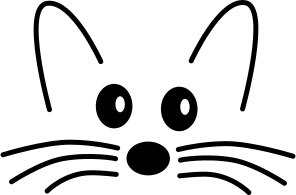
\includegraphics[width=1.4em]{squeak-logo}}}
\iftoshelse{
	\usepackage{marginnote}
		\renewcommand*{\marginfont}{\footnotesize}
	\newcommand{\vartriangleout}{\ifthenelse{\isodd{\thepage}}{\vartriangleright}{\vartriangleleft}}
	\newcommand{\dothisicon}{\fcolorbox{blue!65}{white}{\highlight{$\vartriangleout$}}}
	\newcommand{\dothis}[1]{%
		\noindent\par\noindent
		{\reversemarginpar
			\marginnote{\fcolorbox{blue!65}{white}{\highlight{$\vartriangleout$}}}}
		%\MarginLabel{do this}
		\noindent\emph{#1}
		\nopagebreak}
}{
	\newcommand{\dothisicon}{\raisebox{-.5ex}{
\includegraphics[height=1.2em]{pharo}}}
	\newcommand{\dothis}[1]{%
		\medskip
		\noindent\dothisicon
		\ifx#1\empty\else\quad\emph{#1}\fi
		\par\smallskip\nopagebreak}
}
%===> NEW VERSION <===
% NB: To use this in an individual chapter, you must set:
%\graphicspath{{figures/} {../figures/}}
% at the head of the chapter.  Don't forget the final /
%=============================================================
%:Reader hints (hint)
%
% Indicates a non-obvious consequence 
\newcommand{\hint}[1]{\vspace{1ex}\noindent\fbox{\textsc{Hint}} \emph{#1}}
%=================================================================
% graphics for Morphic handles
\newcommand{\grabHandle}{\raisebox{-0.2ex}{
\includegraphics[width=1em]{blackHandle}}}
\newcommand{\moveHandle}{\raisebox{-0.2ex}{
\includegraphics[width=1em]{moveHandle}}}
\newcommand{\debugHandle}{\raisebox{-0.2ex}{
\includegraphics[width=1em]{debugHandle}}}
%=============================================================
%:Highlighting Important stuff (doublebox)
%
% From Seaside book ...
\newsavebox{\SavedText}
\newlength{\InnerBoxRule}\setlength{\InnerBoxRule}{.75\fboxrule}
\newlength{\OuterBoxRule}\setlength{\OuterBoxRule}{1.5\fboxrule}
\newlength{\BoxSeparation}\setlength{\BoxSeparation}{1.5\fboxrule}
\addtolength{\BoxSeparation}{.5pt}
\newlength{\SaveBoxSep}\setlength{\SaveBoxSep}{2\fboxsep}
%
\newenvironment{doublebox}{\begin{lrbox}{\SavedText}
    \begin{minipage}{.75\textwidth}}
    {\end{minipage}\end{lrbox}\begin{center}
    \setlength{\fboxsep}{\BoxSeparation}\setlength{\fboxrule}{\OuterBoxRule}
    \fbox{\setlength{\fboxsep}{\SaveBoxSep}\setlength{\fboxrule}{\InnerBoxRule}%
      \fbox{\usebox{\SavedText}}}
  \end{center}}
% Use this:
\newcommand{\important}[1]{\begin{doublebox}#1\end{doublebox}}
%=============================================================
%:Section depth
\setcounter{secnumdepth}{2}
%% for this to happen start the file with
%\ifx\wholebook\relax\else
%% $Author$
% $Date$
% $Revision$

% HISTORY:
% 2006-10-31 - Oscar code macros
% ...

%=============================================================
% NB: documentclass must be set in main document.
% Allows book to be generated in multiple formats.
%=============================================================
%:Packages
\usepackage[T1]{fontenc}  %%%%%% really important to get the code directly in the text!
\usepackage{lmodern}
%\usepackage[scaled=0.85]{bookmanx} % needs another scale factor if used with \renewcommand{\sfdefault}{cmbr}
\usepackage{palatino}
\usepackage[scaled=0.85]{helvet}
\usepackage[protrusion,expansion=false]{microtype}
\usepackage{graphicx}
\usepackage{theorem}
\usepackage[english]{babel}
% ON: pdfsync breaks the use of p{width} for tabular columns!
\ifdefined\usepdfsync\usepackage{pdfsync}\fi % Requires texlive 2007
%=============================================================
%:More packages
%Stef should check which ones are used!
%\usepackage{picinpar}
%\usepackage{layout}
%\usepackage{color}
%\usepackage{enum}
%\usepackage{a4wide}
% \usepackage{fancyhdr}
\usepackage{ifthen}
\usepackage{float}
\usepackage{longtable}
\usepackage{makeidx}
\usepackage[nottoc]{tocbibind}
\usepackage{multicol}
\usepackage{booktabs}	% book-style tables
\usepackage{topcapt}	% enables \topcaption
\usepackage{multirow}
\usepackage{tabularx}
%\usepackage[bottom]{footmisc}
\usepackage{xspace}
\usepackage{alltt}
\usepackage{amssymb,textcomp}
\usepackage[usenames,dvipsnames]{color}
%\usepackage{colortbl}
\usepackage[hang]{subfigure}\makeatletter\def\p@subfigure{\thefigure\,}\makeatother
\usepackage{rotating}
\usepackage{enumitem}	% apb: allows more control over tags in enumerations
\usepackage{verbatim}     % for comment environment
\usepackage{varioref}	% for page references that work
\labelformat{footnote}{\thechapter--#1} % to distinguish citations from jurabib
\usepackage{needspace}
\usepackage{isodateo} % enable \isodate
\usepackage[newparttoc]{titlesec}
\usepackage{titletoc}
\usepackage{wrapfig}
\usepackage[
	super,
	citefull=first,
	authorformat={allreversed,and},
	titleformat={commasep,italic}
]{jurabib} % citations as footnotes
\usepackage[
	colorlinks=true,
	linkcolor=black,
	urlcolor=black,
	citecolor=black
]{hyperref}   % should come last
%=============================================================
%:PDF version
\pdfminorversion=3 % Set PDF to 1.3 for Lulu
%=============================================================
%:URL style
\makeatletter
\def\url@leostyle{%
  \@ifundefined{selectfont}{\def\UrlFont{\sf}}{\def\UrlFont{\sffamily}}}
\makeatother
% Now actually use the newly defined style.
\urlstyle{leo}
%=============================================================
%:Booleans
\newboolean{lulu}
\setboolean{lulu}{false}
\newcommand{\ifluluelse}[2]{\ifthenelse{\boolean{lulu}}{#1}{#2}}
%=============================================================
%:Names
\newcommand{\SUnit}{SUnit\xspace}
\newcommand{\sunit}{SUnit\xspace}
\newcommand{\xUnit}{$x$Unit\xspace}
\newcommand{\JUnit}{JUnit\xspace}
\newcommand{\st}{Smalltalk\xspace}
\newcommand{\pharo}{Pharo\xspace} % Use this, not \Pharo
%\newcommand{\sqmap}{SqueakMap\xspace}
\newcommand{\squeak}{Squeak\xspace} % use this, not \Squeak or \sq
\newcommand{\sqsrc}{SqueakSource\xspace}
\newcommand{\sbe}{\url{http://SqueakByExample.org}\xspace}
\newcommand{\pharoweb}{\url{http://pharo-project.org}\xspace}
\newcommand{\pbe}{\url{http://PharoByExample.org}\xspace}
\newcommand{\sba}{\url{http://SquareBracketAssociates.org}\xspace}
\newcommand{\bam}{\lct{Bounc\-ing\-Atoms\-Morph}\xspace}
%=============================================================
%:Markup macros for proof-reading
\usepackage[normalem]{ulem} % for \sout
\usepackage{xcolor}
\newcommand{\ra}{$\rightarrow$}
\newcommand{\ugh}[1]{\textcolor{red}{\uwave{#1}}} % please rephrase
\newcommand{\ins}[1]{\textcolor{blue}{\uline{#1}}} % please insert
\newcommand{\del}[1]{\textcolor{red}{\sout{#1}}} % please delete
\newcommand{\chg}[2]{\textcolor{red}{\sout{#1}}{\ra}\textcolor{blue}{\uline{#2}}} % please change
%=============================================================
%:Editorial comment macros
%\newcommand{\nnbb}[2]{
%    % \fbox{\bfseries\sffamily\scriptsize#1}
%    \fcolorbox{gray}{yellow}{\bfseries\sffamily\scriptsize#1}
%    {\sf\small$\blacktriangleright$\textit{#2}$\blacktriangleleft$}
%   }
\newcommand{\yellowbox}[1]{\fcolorbox{gray}{yellow}{\bfseries\sffamily\scriptsize#1}}
\newcommand{\triangles}[1]{{\sf\small$\blacktriangleright$\textit{#1}$\blacktriangleleft$}}
\newcommand{\nnbb}[2]{\yellowbox{#1} \triangles{#2}}
\newcommand{\fix}{\yellowbox{FIX!}}
\newcommand{\here}{\yellowbox{CONTINUE HERE!}}
% editor macros
\newcommand{\apl}[1]{\nnbb{Alain}{#1}} % Alain
\newcommand{\ab}[1]{\nnbb{Andrew}{#1}} % Black
\newcommand{\sd}[1]{\nnbb{St\'{e}f}{#1}} % Ducasse
\newcommand{\dc}[1]{\nnbb{DamienC}{#1}} % Ducasse
\newcommand{\md}[1]{\nnbb{Marcus}{#1}} % Denker
\newcommand{\on}[1]{\nnbb{Oscar}{#1}} % Nierstrasz
\newcommand{\damien}[1]{\nnbb{Damien}{#1}} % Pollet
\newcommand{\lr}[1]{\nnbb{Lukas}{#1}} % Renggli
\newcommand{\orla}[1]{\nnbb{Orla}{#1}} % Greevy
\newcommand{\alex}[1]{\nnbb{Alex}{#1}} % Bergel
\newcommand{\alx}[1]{\nnbb{Alex}{#1}} % Bergel
\newcommand{\dr}[1]{\nnbb{David}{#1}} % Roethlisberger
\newcommand{\ja}[1]{\nnbb{Jannik}{#1}} % Laval
\newcommand{\jr}[1]{\nnbb{Jorge}{#1}} % Ressia
\newcommand{\jb}[1]{\nnbb{JB}{#1}} % JB
\newcommand{\fp}[1]{\nnbb{Fabrizio}{#1}} % Perin
\newcommand{\michael}[1]{\nnbb{Michael}{#1}} % Davies
\newcommand{\ew}[1]{\nnbb{Erwann}{#1}} % Wernli
\newcommand{\mb}[1]{\nnbb{Martial}{#1}} % Boniou
\newcommand{\hw}[1]{\nnbb{Hernan}{#1}} % Wilkinson
\newcommand{\ben}[1]{\nnbb{Benjamin}{#1}} % Benjamin Van Ryseghem
%=============================================================
%:Abbreviation macros
\newcommand{\ie}{\emph{i.e.},\xspace}
\newcommand{\eg}{\emph{e.g.},\xspace}
\newcommand{\etc}{etc.\xspace}
%=============================================================
%:Cross reference macros
\newcommand{\charef}[1]{Chapter~\ref{cha:#1}\xspace}
\newcommand{\secref}[1]{Section~\ref{sec:#1}\xspace}
\newcommand{\figref}[1]{Figure~\ref{fig:#1}\xspace}
\newcommand{\Figref}[1]{Figure~\ref{fig:#1}\xspace}
\newcommand{\appref}[1]{Appendix~\ref{app:#1}\xspace}
\newcommand{\tabref}[1]{Table~\ref{tab:#1}\xspace}
\newcommand{\faqref}[1]{FAQ~\ref{faq:#1}, p.~\pageref{faq:#1}\xspace}
% APB: I removed trailing \xspace commands from these macros because
% \xspace mostly doesn't work.  If you want a space after your
% references, type one!
% ON: xspace has always worked just fine for me!  Please leave them in.
%
\newcommand{\ruleref}[1]{\ref{rule:#1}\xspace}
%
\newcommand{\egref}[1]{example~\ref{eg:#1}\xspace}
\newcommand{\Egref}[1]{Example~\ref{eg:#1}\xspace}
%
\newcommand{\scrref}[1]{script~\ref{scr:#1}\xspace}
\newcommand{\Scrref}[1]{Script~\ref{scr:#1}\xspace}
\newcommand{\tscrref}[1]{the script~\ref{scr:#1}\xspace}
\newcommand{\Tscrref}[1]{The script~\ref{scr:#1}\xspace}
%
\newcommand{\mthref}[1]{method~\ref{mth:#1}\xspace}
\newcommand{\mthsref}[1]{methods~\ref{mth:#1}\xspace}
\newcommand{\Mthref}[1]{Method~\ref{mth:#1}\xspace}
\newcommand{\tmthref}[1]{the method~\ref{mth:#1}\xspace}
\newcommand{\Tmthref}[1]{The method~\ref{mth:#1}\xspace}
%
\newcommand{\clsref}[1]{class~\ref{cls:#1}\xspace}
\newcommand{\tclsref}[1]{the class~\ref{cls:#1}\xspace}
\newcommand{\Tclsref}[1]{The class~\ref{cls:#1}\xspace}

\newcommand{\chalabel}[1]{\label{cha:#1}}
\newcommand{\seclabel}[1]{\label{sec:#1}}
\newcommand{\figlabel}[1]{\label{fig:#1}}
\newcommand{\tablabel}[1]{\label{tab:#1}}
\newcommand{\rulelabel}[1]{\label{rule:#1}}
\newcommand{\eglabel}[1]{\label{eg:#1}}
\newcommand{\scrlabel}[1]{\label{scr:#1}}
\newcommand{\mthlabel}[1]{\label{mth:#1}}
\newcommand{\clslabel}[1]{\label{cls:#1}}
\newcommand{\faqlabel}[1]{\label{faq:#1}}
%=============================================================
%:Menu item macro
% for menu items, so we can change our minds on how to print them! (apb)
\definecolor{lightgray}{gray}{0.89}
\newcommand{\menu}[1]{{%
	\setlength{\fboxsep}{0pt}%
	\colorbox{lightgray}{{{\upshape\sffamily\strut \,#1\,}}}}}
\newcommand{\link}[1]{{%
	\fontfamily{lmr}\selectfont
 	\upshape{\sffamily \underline{#1}}}}
% For submenu items:
\newcommand{\go}{\,$\triangleright$\,}
% \newcommand{\go}{\,$\blacktriangleright$\,}
% For keyboard shortcuts:
%\newcommand{\short}[1]{\mbox{$\langle${\sc CMD}$\rangle$-#1}\xspace}
\newcommand{\short}[1]{\mbox{{\sc cmd}\hspace{0.08em}--\hspace{0.09em}#1}\xspace}
% For buttons:
\newcommand{\button}[1]{{%
	\setlength{\fboxsep}{0pt}%
	\fbox{{\upshape\sffamily\strut \,#1\,}}}}
% NB: The button macro does not work within captions -- incompatible with xcolor package :-(
\newcommand{\toolsflap}{\textit{Tools} flap\xspace}
%=============================================================
%:Mouse clicks
\newcommand{\click}{click\xspace} % RED
\newcommand{\actclick}{action-click\xspace} % YELLOW
\newcommand{\metaclick}{meta-click\xspace} % BLUE
\newcommand{\Click}{Click\xspace} % RED
\newcommand{\Actclick}{Action-click\xspace} % YELLOW
\newcommand{\Metaclick}{Meta-click\xspace} % BLUE
%=============================================================
%:ToSh macros
\newboolean{tosh}
\setboolean{tosh}{false}
\newcommand{\iftoshelse}[2]{\ifthenelse{\boolean{tosh}}{#1}{#2}}
%=============================================================
%:ToSh colors
%\newcommand{\highlightcolor}{\color{blue!65}}
%\newcommand{\boxcolor}{\color{gray!25}}
\newcommand{\highlight}[1]{\textcolor{blue!65}{#1}}
%\newcommand{\codecolor}{\color{blue!65}}
%%\setlength{\fboxrule}{2pt}
%\newcommand{\asPict}[1]{%
%	{\Large\highlight{#1}}}
%=============================================================
%:Reader cues (do this)
%
% Indicate something the reader should try out.
% \newcommand{\dothisicon}{\raisebox{-.5ex}{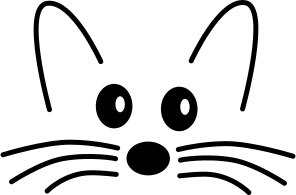
\includegraphics[width=1.4em]{squeak-logo}}}
\iftoshelse{
	\usepackage{marginnote}
		\renewcommand*{\marginfont}{\footnotesize}
	\newcommand{\vartriangleout}{\ifthenelse{\isodd{\thepage}}{\vartriangleright}{\vartriangleleft}}
	\newcommand{\dothisicon}{\fcolorbox{blue!65}{white}{\highlight{$\vartriangleout$}}}
	\newcommand{\dothis}[1]{%
		\noindent\par\noindent
		{\reversemarginpar
			\marginnote{\fcolorbox{blue!65}{white}{\highlight{$\vartriangleout$}}}}
		%\MarginLabel{do this}
		\noindent\emph{#1}
		\nopagebreak}
}{
	\newcommand{\dothisicon}{\raisebox{-.5ex}{
\includegraphics[height=1.2em]{pharo}}}
	\newcommand{\dothis}[1]{%
		\medskip
		\noindent\dothisicon
		\ifx#1\empty\else\quad\emph{#1}\fi
		\par\smallskip\nopagebreak}
}
%===> NEW VERSION <===
% NB: To use this in an individual chapter, you must set:
%\graphicspath{{figures/} {../figures/}}
% at the head of the chapter.  Don't forget the final /
%=============================================================
%:Reader hints (hint)
%
% Indicates a non-obvious consequence 
\newcommand{\hint}[1]{\vspace{1ex}\noindent\fbox{\textsc{Hint}} \emph{#1}}
%=================================================================
% graphics for Morphic handles
\newcommand{\grabHandle}{\raisebox{-0.2ex}{
\includegraphics[width=1em]{blackHandle}}}
\newcommand{\moveHandle}{\raisebox{-0.2ex}{
\includegraphics[width=1em]{moveHandle}}}
\newcommand{\debugHandle}{\raisebox{-0.2ex}{
\includegraphics[width=1em]{debugHandle}}}
%=============================================================
%:Highlighting Important stuff (doublebox)
%
% From Seaside book ...
\newsavebox{\SavedText}
\newlength{\InnerBoxRule}\setlength{\InnerBoxRule}{.75\fboxrule}
\newlength{\OuterBoxRule}\setlength{\OuterBoxRule}{1.5\fboxrule}
\newlength{\BoxSeparation}\setlength{\BoxSeparation}{1.5\fboxrule}
\addtolength{\BoxSeparation}{.5pt}
\newlength{\SaveBoxSep}\setlength{\SaveBoxSep}{2\fboxsep}
%
\newenvironment{doublebox}{\begin{lrbox}{\SavedText}
    \begin{minipage}{.75\textwidth}}
    {\end{minipage}\end{lrbox}\begin{center}
    \setlength{\fboxsep}{\BoxSeparation}\setlength{\fboxrule}{\OuterBoxRule}
    \fbox{\setlength{\fboxsep}{\SaveBoxSep}\setlength{\fboxrule}{\InnerBoxRule}%
      \fbox{\usebox{\SavedText}}}
  \end{center}}
% Use this:
\newcommand{\important}[1]{\begin{doublebox}#1\end{doublebox}}
%=============================================================
%:Section depth
\setcounter{secnumdepth}{2}
%% for this to happen start the file with
%\ifx\wholebook\relax\else
%% $Author$
% $Date$
% $Revision$

% HISTORY:
% 2006-10-31 - Oscar code macros
% ...

%=============================================================
% NB: documentclass must be set in main document.
% Allows book to be generated in multiple formats.
%=============================================================
%:Packages
\usepackage[T1]{fontenc}  %%%%%% really important to get the code directly in the text!
\usepackage{lmodern}
%\usepackage[scaled=0.85]{bookmanx} % needs another scale factor if used with \renewcommand{\sfdefault}{cmbr}
\usepackage{palatino}
\usepackage[scaled=0.85]{helvet}
\usepackage[protrusion,expansion=false]{microtype}
\usepackage{graphicx}
\usepackage{theorem}
\usepackage[english]{babel}
% ON: pdfsync breaks the use of p{width} for tabular columns!
\ifdefined\usepdfsync\usepackage{pdfsync}\fi % Requires texlive 2007
%=============================================================
%:More packages
%Stef should check which ones are used!
%\usepackage{picinpar}
%\usepackage{layout}
%\usepackage{color}
%\usepackage{enum}
%\usepackage{a4wide}
% \usepackage{fancyhdr}
\usepackage{ifthen}
\usepackage{float}
\usepackage{longtable}
\usepackage{makeidx}
\usepackage[nottoc]{tocbibind}
\usepackage{multicol}
\usepackage{booktabs}	% book-style tables
\usepackage{topcapt}	% enables \topcaption
\usepackage{multirow}
\usepackage{tabularx}
%\usepackage[bottom]{footmisc}
\usepackage{xspace}
\usepackage{alltt}
\usepackage{amssymb,textcomp}
\usepackage[usenames,dvipsnames]{color}
%\usepackage{colortbl}
\usepackage[hang]{subfigure}\makeatletter\def\p@subfigure{\thefigure\,}\makeatother
\usepackage{rotating}
\usepackage{enumitem}	% apb: allows more control over tags in enumerations
\usepackage{verbatim}     % for comment environment
\usepackage{varioref}	% for page references that work
\labelformat{footnote}{\thechapter--#1} % to distinguish citations from jurabib
\usepackage{needspace}
\usepackage{isodateo} % enable \isodate
\usepackage[newparttoc]{titlesec}
\usepackage{titletoc}
\usepackage{wrapfig}
\usepackage[
	super,
	citefull=first,
	authorformat={allreversed,and},
	titleformat={commasep,italic}
]{jurabib} % citations as footnotes
\usepackage[
	colorlinks=true,
	linkcolor=black,
	urlcolor=black,
	citecolor=black
]{hyperref}   % should come last
%=============================================================
%:PDF version
\pdfminorversion=3 % Set PDF to 1.3 for Lulu
%=============================================================
%:URL style
\makeatletter
\def\url@leostyle{%
  \@ifundefined{selectfont}{\def\UrlFont{\sf}}{\def\UrlFont{\sffamily}}}
\makeatother
% Now actually use the newly defined style.
\urlstyle{leo}
%=============================================================
%:Booleans
\newboolean{lulu}
\setboolean{lulu}{false}
\newcommand{\ifluluelse}[2]{\ifthenelse{\boolean{lulu}}{#1}{#2}}
%=============================================================
%:Names
\newcommand{\SUnit}{SUnit\xspace}
\newcommand{\sunit}{SUnit\xspace}
\newcommand{\xUnit}{$x$Unit\xspace}
\newcommand{\JUnit}{JUnit\xspace}
\newcommand{\st}{Smalltalk\xspace}
\newcommand{\pharo}{Pharo\xspace} % Use this, not \Pharo
%\newcommand{\sqmap}{SqueakMap\xspace}
\newcommand{\squeak}{Squeak\xspace} % use this, not \Squeak or \sq
\newcommand{\sqsrc}{SqueakSource\xspace}
\newcommand{\sbe}{\url{http://SqueakByExample.org}\xspace}
\newcommand{\pharoweb}{\url{http://pharo-project.org}\xspace}
\newcommand{\pbe}{\url{http://PharoByExample.org}\xspace}
\newcommand{\sba}{\url{http://SquareBracketAssociates.org}\xspace}
\newcommand{\bam}{\lct{Bounc\-ing\-Atoms\-Morph}\xspace}
%=============================================================
%:Markup macros for proof-reading
\usepackage[normalem]{ulem} % for \sout
\usepackage{xcolor}
\newcommand{\ra}{$\rightarrow$}
\newcommand{\ugh}[1]{\textcolor{red}{\uwave{#1}}} % please rephrase
\newcommand{\ins}[1]{\textcolor{blue}{\uline{#1}}} % please insert
\newcommand{\del}[1]{\textcolor{red}{\sout{#1}}} % please delete
\newcommand{\chg}[2]{\textcolor{red}{\sout{#1}}{\ra}\textcolor{blue}{\uline{#2}}} % please change
%=============================================================
%:Editorial comment macros
%\newcommand{\nnbb}[2]{
%    % \fbox{\bfseries\sffamily\scriptsize#1}
%    \fcolorbox{gray}{yellow}{\bfseries\sffamily\scriptsize#1}
%    {\sf\small$\blacktriangleright$\textit{#2}$\blacktriangleleft$}
%   }
\newcommand{\yellowbox}[1]{\fcolorbox{gray}{yellow}{\bfseries\sffamily\scriptsize#1}}
\newcommand{\triangles}[1]{{\sf\small$\blacktriangleright$\textit{#1}$\blacktriangleleft$}}
\newcommand{\nnbb}[2]{\yellowbox{#1} \triangles{#2}}
\newcommand{\fix}{\yellowbox{FIX!}}
\newcommand{\here}{\yellowbox{CONTINUE HERE!}}
% editor macros
\newcommand{\apl}[1]{\nnbb{Alain}{#1}} % Alain
\newcommand{\ab}[1]{\nnbb{Andrew}{#1}} % Black
\newcommand{\sd}[1]{\nnbb{St\'{e}f}{#1}} % Ducasse
\newcommand{\dc}[1]{\nnbb{DamienC}{#1}} % Ducasse
\newcommand{\md}[1]{\nnbb{Marcus}{#1}} % Denker
\newcommand{\on}[1]{\nnbb{Oscar}{#1}} % Nierstrasz
\newcommand{\damien}[1]{\nnbb{Damien}{#1}} % Pollet
\newcommand{\lr}[1]{\nnbb{Lukas}{#1}} % Renggli
\newcommand{\orla}[1]{\nnbb{Orla}{#1}} % Greevy
\newcommand{\alex}[1]{\nnbb{Alex}{#1}} % Bergel
\newcommand{\alx}[1]{\nnbb{Alex}{#1}} % Bergel
\newcommand{\dr}[1]{\nnbb{David}{#1}} % Roethlisberger
\newcommand{\ja}[1]{\nnbb{Jannik}{#1}} % Laval
\newcommand{\jr}[1]{\nnbb{Jorge}{#1}} % Ressia
\newcommand{\jb}[1]{\nnbb{JB}{#1}} % JB
\newcommand{\fp}[1]{\nnbb{Fabrizio}{#1}} % Perin
\newcommand{\michael}[1]{\nnbb{Michael}{#1}} % Davies
\newcommand{\ew}[1]{\nnbb{Erwann}{#1}} % Wernli
\newcommand{\mb}[1]{\nnbb{Martial}{#1}} % Boniou
\newcommand{\hw}[1]{\nnbb{Hernan}{#1}} % Wilkinson
\newcommand{\ben}[1]{\nnbb{Benjamin}{#1}} % Benjamin Van Ryseghem
%=============================================================
%:Abbreviation macros
\newcommand{\ie}{\emph{i.e.},\xspace}
\newcommand{\eg}{\emph{e.g.},\xspace}
\newcommand{\etc}{etc.\xspace}
%=============================================================
%:Cross reference macros
\newcommand{\charef}[1]{Chapter~\ref{cha:#1}\xspace}
\newcommand{\secref}[1]{Section~\ref{sec:#1}\xspace}
\newcommand{\figref}[1]{Figure~\ref{fig:#1}\xspace}
\newcommand{\Figref}[1]{Figure~\ref{fig:#1}\xspace}
\newcommand{\appref}[1]{Appendix~\ref{app:#1}\xspace}
\newcommand{\tabref}[1]{Table~\ref{tab:#1}\xspace}
\newcommand{\faqref}[1]{FAQ~\ref{faq:#1}, p.~\pageref{faq:#1}\xspace}
% APB: I removed trailing \xspace commands from these macros because
% \xspace mostly doesn't work.  If you want a space after your
% references, type one!
% ON: xspace has always worked just fine for me!  Please leave them in.
%
\newcommand{\ruleref}[1]{\ref{rule:#1}\xspace}
%
\newcommand{\egref}[1]{example~\ref{eg:#1}\xspace}
\newcommand{\Egref}[1]{Example~\ref{eg:#1}\xspace}
%
\newcommand{\scrref}[1]{script~\ref{scr:#1}\xspace}
\newcommand{\Scrref}[1]{Script~\ref{scr:#1}\xspace}
\newcommand{\tscrref}[1]{the script~\ref{scr:#1}\xspace}
\newcommand{\Tscrref}[1]{The script~\ref{scr:#1}\xspace}
%
\newcommand{\mthref}[1]{method~\ref{mth:#1}\xspace}
\newcommand{\mthsref}[1]{methods~\ref{mth:#1}\xspace}
\newcommand{\Mthref}[1]{Method~\ref{mth:#1}\xspace}
\newcommand{\tmthref}[1]{the method~\ref{mth:#1}\xspace}
\newcommand{\Tmthref}[1]{The method~\ref{mth:#1}\xspace}
%
\newcommand{\clsref}[1]{class~\ref{cls:#1}\xspace}
\newcommand{\tclsref}[1]{the class~\ref{cls:#1}\xspace}
\newcommand{\Tclsref}[1]{The class~\ref{cls:#1}\xspace}

\newcommand{\chalabel}[1]{\label{cha:#1}}
\newcommand{\seclabel}[1]{\label{sec:#1}}
\newcommand{\figlabel}[1]{\label{fig:#1}}
\newcommand{\tablabel}[1]{\label{tab:#1}}
\newcommand{\rulelabel}[1]{\label{rule:#1}}
\newcommand{\eglabel}[1]{\label{eg:#1}}
\newcommand{\scrlabel}[1]{\label{scr:#1}}
\newcommand{\mthlabel}[1]{\label{mth:#1}}
\newcommand{\clslabel}[1]{\label{cls:#1}}
\newcommand{\faqlabel}[1]{\label{faq:#1}}
%=============================================================
%:Menu item macro
% for menu items, so we can change our minds on how to print them! (apb)
\definecolor{lightgray}{gray}{0.89}
\newcommand{\menu}[1]{{%
	\setlength{\fboxsep}{0pt}%
	\colorbox{lightgray}{{{\upshape\sffamily\strut \,#1\,}}}}}
\newcommand{\link}[1]{{%
	\fontfamily{lmr}\selectfont
 	\upshape{\sffamily \underline{#1}}}}
% For submenu items:
\newcommand{\go}{\,$\triangleright$\,}
% \newcommand{\go}{\,$\blacktriangleright$\,}
% For keyboard shortcuts:
%\newcommand{\short}[1]{\mbox{$\langle${\sc CMD}$\rangle$-#1}\xspace}
\newcommand{\short}[1]{\mbox{{\sc cmd}\hspace{0.08em}--\hspace{0.09em}#1}\xspace}
% For buttons:
\newcommand{\button}[1]{{%
	\setlength{\fboxsep}{0pt}%
	\fbox{{\upshape\sffamily\strut \,#1\,}}}}
% NB: The button macro does not work within captions -- incompatible with xcolor package :-(
\newcommand{\toolsflap}{\textit{Tools} flap\xspace}
%=============================================================
%:Mouse clicks
\newcommand{\click}{click\xspace} % RED
\newcommand{\actclick}{action-click\xspace} % YELLOW
\newcommand{\metaclick}{meta-click\xspace} % BLUE
\newcommand{\Click}{Click\xspace} % RED
\newcommand{\Actclick}{Action-click\xspace} % YELLOW
\newcommand{\Metaclick}{Meta-click\xspace} % BLUE
%=============================================================
%:ToSh macros
\newboolean{tosh}
\setboolean{tosh}{false}
\newcommand{\iftoshelse}[2]{\ifthenelse{\boolean{tosh}}{#1}{#2}}
%=============================================================
%:ToSh colors
%\newcommand{\highlightcolor}{\color{blue!65}}
%\newcommand{\boxcolor}{\color{gray!25}}
\newcommand{\highlight}[1]{\textcolor{blue!65}{#1}}
%\newcommand{\codecolor}{\color{blue!65}}
%%\setlength{\fboxrule}{2pt}
%\newcommand{\asPict}[1]{%
%	{\Large\highlight{#1}}}
%=============================================================
%:Reader cues (do this)
%
% Indicate something the reader should try out.
% \newcommand{\dothisicon}{\raisebox{-.5ex}{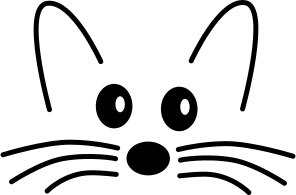
\includegraphics[width=1.4em]{squeak-logo}}}
\iftoshelse{
	\usepackage{marginnote}
		\renewcommand*{\marginfont}{\footnotesize}
	\newcommand{\vartriangleout}{\ifthenelse{\isodd{\thepage}}{\vartriangleright}{\vartriangleleft}}
	\newcommand{\dothisicon}{\fcolorbox{blue!65}{white}{\highlight{$\vartriangleout$}}}
	\newcommand{\dothis}[1]{%
		\noindent\par\noindent
		{\reversemarginpar
			\marginnote{\fcolorbox{blue!65}{white}{\highlight{$\vartriangleout$}}}}
		%\MarginLabel{do this}
		\noindent\emph{#1}
		\nopagebreak}
}{
	\newcommand{\dothisicon}{\raisebox{-.5ex}{
\includegraphics[height=1.2em]{pharo}}}
	\newcommand{\dothis}[1]{%
		\medskip
		\noindent\dothisicon
		\ifx#1\empty\else\quad\emph{#1}\fi
		\par\smallskip\nopagebreak}
}
%===> NEW VERSION <===
% NB: To use this in an individual chapter, you must set:
%\graphicspath{{figures/} {../figures/}}
% at the head of the chapter.  Don't forget the final /
%=============================================================
%:Reader hints (hint)
%
% Indicates a non-obvious consequence 
\newcommand{\hint}[1]{\vspace{1ex}\noindent\fbox{\textsc{Hint}} \emph{#1}}
%=================================================================
% graphics for Morphic handles
\newcommand{\grabHandle}{\raisebox{-0.2ex}{
\includegraphics[width=1em]{blackHandle}}}
\newcommand{\moveHandle}{\raisebox{-0.2ex}{
\includegraphics[width=1em]{moveHandle}}}
\newcommand{\debugHandle}{\raisebox{-0.2ex}{
\includegraphics[width=1em]{debugHandle}}}
%=============================================================
%:Highlighting Important stuff (doublebox)
%
% From Seaside book ...
\newsavebox{\SavedText}
\newlength{\InnerBoxRule}\setlength{\InnerBoxRule}{.75\fboxrule}
\newlength{\OuterBoxRule}\setlength{\OuterBoxRule}{1.5\fboxrule}
\newlength{\BoxSeparation}\setlength{\BoxSeparation}{1.5\fboxrule}
\addtolength{\BoxSeparation}{.5pt}
\newlength{\SaveBoxSep}\setlength{\SaveBoxSep}{2\fboxsep}
%
\newenvironment{doublebox}{\begin{lrbox}{\SavedText}
    \begin{minipage}{.75\textwidth}}
    {\end{minipage}\end{lrbox}\begin{center}
    \setlength{\fboxsep}{\BoxSeparation}\setlength{\fboxrule}{\OuterBoxRule}
    \fbox{\setlength{\fboxsep}{\SaveBoxSep}\setlength{\fboxrule}{\InnerBoxRule}%
      \fbox{\usebox{\SavedText}}}
  \end{center}}
% Use this:
\newcommand{\important}[1]{\begin{doublebox}#1\end{doublebox}}
%=============================================================
%:Section depth
\setcounter{secnumdepth}{2}
%% for this to happen start the file with
%\ifx\wholebook\relax\else
%\input{../common.tex}
%\begin{document}
%\fi
% and terminate by
% \ifx\wholebook\relax\else\end{document}\fi

\DeclareGraphicsExtensions{.pdf, .jpg, .png}
%=============================================================
%:PDF setup
\hypersetup{
%   a4paper,
%   pdfstartview=FitV,
%   colorlinks,
%   linkcolor=darkblue,
%   citecolor=darkblue,
   pdftitle={Pharo by Example},
   pdfauthor={Andrew P. Black, St\'ephane Ducasse,	Oscar Nierstrasz,
Damien Pollet},
   pdfkeywords={Smalltalk, Squeak, Object-Oriented Programming, OOP},
   pdfsubject={Computer Science}
}
%=============================================================
%:Page layout and appearance
%
% \renewcommand{\headrulewidth}{0pt}
\renewcommand{\chaptermark}[1]{\markboth{#1}{}}
\renewcommand{\sectionmark}[1]{\markright{\thesection\ #1}}
\renewpagestyle{plain}[\small\itshape]{%
	\setheadrule{0pt}%
	\sethead[][][]{}{}{}%
	\setfoot[][][]{}{}{}}
\renewpagestyle{headings}[\small\itshape]{%
	\setheadrule{0pt}%
	\setmarks{chapter}{section}%
	\sethead[\thepage][][\chaptertitle]{\sectiontitle}{}{\thepage}%
	\setfoot[][][]{}{}{}}
%=============================================================
%:Title section setup and TOC numbering depth
\setcounter{secnumdepth}{1}
\setcounter{tocdepth}{1}
\titleformat{\part}[display]{\centering}{\huge\partname\ \thepart}{1em}{\Huge\textbf}[]
\titleformat{\chapter}[display]{}{\huge\chaptertitlename\ \thechapter}{1em}{\Huge\raggedright\textbf}[]
\titlecontents{part}[3pc]{%
		\pagebreak[2]\addvspace{1em plus.4em minus.2em}%
		\leavevmode\large\bfseries}
	{\contentslabel{3pc}}{\hspace*{-3pc}}
	{}[\nopagebreak]
\titlecontents{chapter}[3pc]{%
		\pagebreak[0]\addvspace{1em plus.2em minus.2em}%
		\leavevmode\bfseries}
	{\contentslabel{3pc}}{}
	{\hfill\contentspage}[\nopagebreak]
\dottedcontents{section}[3pc]{}{3pc}{1pc}
\dottedcontents{subsection}[3pc]{}{0pc}{1pc}
% \dottedcontents{subsection}[4.5em]{}{0pt}{1pc}
% Make \cleardoublepage insert really blank pages http://www.tex.ac.uk/cgi-bin/texfaq2html?label=reallyblank
\let\origdoublepage\cleardoublepage
\newcommand{\clearemptydoublepage}{%
  \clearpage
  {\pagestyle{empty}\origdoublepage}}
\let\cleardoublepage\clearemptydoublepage % see http://www.tex.ac.uk/cgi-bin/texfaq2html?label=patch
%=============================================================
%:FAQ macros (for FAQ chapter)
\newtheorem{faq}{FAQ}
\newcommand{\answer}{\paragraph{Answer}\ }
%=============================================================
%:Listings package configuration
% \newcommand{\caret}{\makebox{\raisebox{0.4ex}{\footnotesize{$\wedge$}}}}
\newcommand{\caret}{\^\,}
\newcommand{\escape}{{\sf \textbackslash}}
\definecolor{source}{gray}{0.95}
\usepackage{listings}
\lstdefinelanguage{Smalltalk}{
%  morekeywords={self,super,true,false,nil,thisContext}, % This is overkill
  morestring=[d]',
  morecomment=[s]{"}{"},
  alsoletter={\#:},
  escapechar={!},
  literate=
    {BANG}{!}1
    {CARET}{\^}1
    {UNDERSCORE}{\_}1
    {\\st}{Smalltalk}9 % convenience -- in case \st occurs in code
    % {'}{{\textquotesingle}}1 % replaced by upquote=true in \lstset
    {_}{{$\leftarrow$}}1
    {>>>}{{\sep}}1
    {^}{{$\uparrow$}}1
    {~}{{$\sim$}}1
    {-}{{\texttt{-}}}1 %{\textminus}}1 %{-}{\hspace{-0.13em}}{-}}1  % the goal is to make - the same width as +
    % {+}{\sf+}1 %{\raisebox{0.08ex}{+}}}1      % and to raise + off the baseline to match -
    {-->}{{\quad$\longrightarrow$\quad}}3
	, % Don't forget the comma at the end!
  tabsize=4
}[keywords,comments,strings]

\lstset{language=Smalltalk,
	basicstyle=\sffamily,
	keywordstyle=\color{black}\bfseries,
	% stringstyle=\ttfamily, % Ugly! do we really want this? -- on
	mathescape=true,
	showstringspaces=false,
	keepspaces=true,
	breaklines=true,
	breakautoindent=true,
	backgroundcolor=\color{source},
	lineskip={-1pt}, % Ugly hack
	upquote=true, % straight quote; requires textcomp package
	columns=fullflexible} % no fixed width fonts
% In-line code (literal)
% Normally use this for all in-line code:
\newcommand{\ct}{\lstinline[mathescape=false,backgroundcolor=\color{white},basicstyle={\sffamily\upshape}]}
% apb 2007.8.28 added the \upshape declaration to avoid getting italicized code in \dothis{ } sections.
% In-line code (latex enabled)
% Use this only in special situations where \ct does not work
% (within section headings ...):
\newcommand{\lct}[1]{{\textsf{\textup{#1}}}}
% Use these for system categories and protocols:
\newcommand{\scat}[1]{\emph{\textsf{#1}}\xspace}
\newcommand{\pkg}[1]{\emph{\textsf{#1}}\xspace}
\newcommand{\prot}[1]{\emph{\textsf{#1}}\xspace}
% Code environments
% NB: the arg is for tests
% Only code and example environments may be tests
\lstnewenvironment{code}[1]{%
	\lstset{%
		% frame=lines,
		frame=single,
		framerule=0pt,
		mathescape=false
	}
}{}
\def\ignoredollar#1{}
%=============================================================
%:Code environments (method, script ...)
% NB: the third arg is for tests
% Only code and example environments may be tests
\lstnewenvironment{example}[3][defaultlabel]{%
	\renewcommand{\lstlistingname}{Example}%
	\lstset{
		% frame=lines,
		frame=single,
		framerule=0pt,
		mathescape=false,
		caption={\emph{#2}},
		label={eg:#1}
	}
}{}
\lstnewenvironment{script}[2][defaultlabel]{%
\renewcommand{\lstlistingname}{Script}%
	\lstset{
		% frame=lines,
		frame=single,
		framerule=0pt,
		mathescape=false,
		name={Script},
		caption={\emph{#2}},
		label={scr:#1}
	}
}{}
\lstnewenvironment{method}[2][defaultlabel]{%
	\renewcommand{\lstlistingname}{Method}%
	\lstset{
		% frame=lines,
		frame=single,
		framerule=0pt,
		mathescape=false,
		name={Method},
		caption={\emph{#2}},
		label={mth:#1}
	}
}{}
\lstnewenvironment{methods}[2][defaultlabel]{% just for multiple methods at once
	\renewcommand{\lstlistingname}{Methods}%
	\lstset{
		% frame=lines,
		frame=single,
		framerule=0pt,
		mathescape=false,
		name={Method},
		caption={\emph{#2}},
		label={mth:#1}
	}
}{}
\lstnewenvironment{numMethod}[2][defaultlabel]{%
	\renewcommand{\lstlistingname}{Method}%
	\lstset{
		numbers=left,
		numberstyle={\tiny\sffamily},
		% frame=lines,
		frame=single,
		framerule=0pt,
		mathescape=false,
		name={Method},
		caption={\emph{#2}},
		label={mth:#1}
	}
}{}
\lstnewenvironment{classdef}[2][defaultlabel]{%
	\renewcommand{\lstlistingname}{Class}%
	\lstset{
		% frame=lines,
		frame=single,
		framerule=0pt,
		mathescape=false,
		name={Class},
		caption={\emph{#2}},
		label={cls:#1}
	}
}{}
%=============================================================
%:Reserving space
% Usually need one more line than the actual lines of code
\newcommand{\needlines}[1]{\Needspace{#1\baselineskip}}
%=============================================================
%:Indexing macros
% Macros ending with "ind" generate text as well as an index entry
% Macros ending with "index" *only* generate an index entry
\newcommand{\ind}[1]{\index{#1}#1\xspace} % plain text
\newcommand{\subind}[2]{\index{#1!#2}#2\xspace} % show #2, subindex under #1
\newcommand{\emphind}[1]{\index{#1}\emph{#1}\xspace} % emph #1
\newcommand{\emphsubind}[2]{\index{#1!#2}\emph{#2}\xspace} % show emph #2, subindex inder #1
\newcommand{\scatind}[1]{\index{#1@\textsf{#1} (category)}\scat{#1}} % category
\newcommand{\pkgind}[1]{\index{#1@\textsf{#1} (package)}\pkg{#1}} % package
\newcommand{\protind}[1]{\index{#1@\textsf{#1} (protocol)}\prot{#1}} % protocol
\newcommand{\clsind}[1]{\index{#1@\textsf{#1} (class)}\ct{#1}\xspace}
% \newcommand{\clsind}[1]{\index{#1!\#@(class)}\ct{#1}\xspace} % class
\newcommand{\clsindplural}[1]{\index{#1!\#@(class)}\ct{#1}s\xspace} % class
\newcommand{\cvind}[1]{\index{#1@\textsf{#1} (class variable)}\ct{#1}\xspace} % class var
\newcommand{\glbind}[1]{\index{#1@\textsf{#1} (global)}\ct{#1}\xspace} % global
\newcommand{\patind}[1]{\index{#1@#1 (pattern)}\ct{#1}\xspace} % pattern
\newcommand{\pvind}[1]{\index{#1@\textsf{#1} (pseudo variable)}\ct{#1}\xspace} % pseudo var
\newcommand{\clsmthind}[2]{\index{#1!#2@\ct{#2}}\ct{#1>>>#2}\xspace} % class + method name
\newcommand{\mthind}[2]{\index{#1!#2@\ct{#2}}\ct{#2}\xspace} % show method name only
\newcommand{\lmthind}[2]{\index{#1!#2@\ct{#2}}\lct{#2}\xspace} % show method name only
\newcommand{\cmind}[2]{\index{#1!#2@\ct{#2}}\ct{#1>>>#2}\xspace} % show class>>method
\newcommand{\lcmind}[2]{\index{#1!#2@\ct{#2}}\lct{#1>>>#2}\xspace} % show class>>method
\newcommand{\toolsflapind}{\index{Tools flap}\toolsflap} % index tools flap
% The following only generate an index entry:
% \newcommand{\clsindex}[1]{\index{#1@\textsf{#1} (class)}}
\newcommand{\clsindex}[1]{\index{#1!\#@(class)}} % class
\newcommand{\mthindex}[2]{\index{#1!#2@\ct{#2}}} % method
\newcommand{\cmindex}[2]{\index{#1!#2@\ct{#2}}} % class>>method
\newcommand{\cvindex}[1]{\index{#1@\textsf{#1} (class variable)}} % class var
\newcommand{\glbindex}[1]{\index{#1@\textsf{#1} (global)}}% global
\newcommand{\pvindex}[1]{\index{#1@\textsf{#1} (pseudo variable)}}% pseudo var
\newcommand{\seeindex}[2]{\index{#1|see{#2}}} % #1, see #2
\newcommand{\scatindex}[1]{\index{#1@\textsf{#1} (category)}} % category
\newcommand{\pkgindex}[1]{\index{#1@\textsf{#1} (package)}} % package
\newcommand{\protindex}[1]{\index{#1@\textsf{#1} (protocol)}} % protocol
% How can we have the main entry page numbers in bold yet not break the hyperlink?
\newcommand{\boldidx}[1]{{\bf #1}} % breaks hyperlink
%\newcommand{\indmain}[1]{\index{#1|boldidx}#1\xspace} % plain text, main entry
%\newcommand{\emphsubindmain}[2]{\index{#1!#2|boldidx}\emph{#2}\xspace} % subindex, main entry
%\newcommand{\subindmain}[2]{\index{#1!#2|boldidx}#2\xspace} % subindex, main entry
%\newcommand{\clsindmain}[1]{\index{#1@\textsf{#1} (class)|boldidx}\ct{#1}\xspace}
%\newcommand{\clsindmain}[1]{\index{#1!\#@(class)|boldidx}\ct{#1}\xspace} % class main
%\newcommand{\indexmain}[1]{\index{#1|boldidx}} % main index entry only
\newcommand{\indmain}[1]{\index{#1}#1\xspace} % The main index entry for this item
\newcommand{\emphsubindmain}[2]{\index{#1!#2}\emph{#2}\xspace} % subindex, main entry
\newcommand{\subindmain}[2]{\index{#1!#2}#2\xspace} % subindex, main entry
%\newcommand{\clsindmain}[1]{\index{#1@\textsf{#1} (class)}\ct{#1}\xspace}
\newcommand{\clsindmain}[1]{\index{#1!\#@(class)}\ct{#1}\xspace} % class main
\newcommand{\clsindexmain}[1]{\index{#1!\#@(class)}} % class main index only
\newcommand{\indexmain}[1]{\index{#1}} 
%=============================================================
%:Code macros
% some constants
\newcommand{\codesize}{\small}
\newcommand{\codefont}{\sffamily}
%\newcommand{\cat}[1]{\textit{In category #1}}%%To remove later
\newlength{\scriptindent}
\setlength{\scriptindent}{.3cm}
%% Method presentation constants
\newlength{\methodindent}
\newlength{\methodwordlength}
\newlength{\aftermethod}
\setlength{\methodindent}{0.2cm}
\settowidth{\methodwordlength}{\ M\'ethode\ }
%=============================================================
%:Smalltalk macros
%\newcommand{\sep}{{$\gg$}}
\newcommand{\sep}{\mbox{>>}}
\newcommand{\self}{\lct{self}\xspace}
\newcommand{\super}{\lct{super}\xspace}
\newcommand{\nil}{\lct{nil}\xspace}
%=============================================================
% be less conservative about float placement
% these commands are from http://www.tex.ac.uk/cgi-bin/texfaq2html?label=floats
\renewcommand{\topfraction}{.9}
\renewcommand{\bottomfraction}{.9}
\renewcommand{\textfraction}{.1}
\renewcommand{\floatpagefraction}{.85}
\renewcommand{\dbltopfraction}{.66}
\renewcommand{\dblfloatpagefraction}{.85}
\setcounter{topnumber}{9}
\setcounter{bottomnumber}{9}
\setcounter{totalnumber}{20}
\setcounter{dbltopnumber}{9}
%=============================================================
% Give information from each chapter's author
\newcommand{\contact}[2]{\textbf{#1} \textsf{(#2)}}

\newcommand{\chapterauthor}[1]{\emph{with the participation of:\\#1}\\}

\newcommand{\authornoury}{\contact{Noury Bouraqadi}{bouraqadi@gmail.com}}
\newcommand{\authordamienc}{\contact{Damien Cassou}{damien.cassou@gmail.com}}
\newcommand{\authoroscar}{\contact{Oscar Nierstrasz}{oscar.nierstrasz@acm.org}}
\newcommand{\authorsteph}{\contact{St\'ephane Ducasse}{stephane.ducasse@inria.fr}}
\newcommand{\authoralex}{\contact{Alexandre Bergel}{alexandre@bergel.eu}}
\newcommand{\authorolivier}{\contact{Olivier Auverlot}{olivier.auverlot@inria.fr}}
\newcommand{\authornicolas}{\contact{Nicolas Cellier}{nicolas.cellier.aka.nice@gmail.com}}
\newcommand{\authormarcus}{\contact{Marcus Denker}{marcus.denker@inria.fr}}
\newcommand{\authoralain}{\contact{Alain Plantec}{alain.plantec@univ-brest.fr}}
\newcommand{\authordale}{\contact{Dale Henrichs}{dale.henrichs@gemstone.com}}
\newcommand{\authormariano}{\contact{Mariano Martinez Peck}{marianopeck@gmail.com}}
\newcommand{\authorsven}{\contact{Sven Van Caekenberghe}{sven@beta9.be}}
\newcommand{\authorlukas}{\contact{Lukas Renggli}{renggli@gmail.com}}

%=============================================================
% apb doesn't like paragraphs to run in to each other without a break
\parskip 1ex
%=============================================================
%:Stuff to check, merge or deprecate
%\setlength{\marginparsep}{2mm}
%\renewcommand{\baselinestretch}{1.1}
%=============================================================

%\begin{document}
%\fi
% and terminate by
% \ifx\wholebook\relax\else\end{document}\fi

\DeclareGraphicsExtensions{.pdf, .jpg, .png}
%=============================================================
%:PDF setup
\hypersetup{
%   a4paper,
%   pdfstartview=FitV,
%   colorlinks,
%   linkcolor=darkblue,
%   citecolor=darkblue,
   pdftitle={Pharo by Example},
   pdfauthor={Andrew P. Black, St\'ephane Ducasse,	Oscar Nierstrasz,
Damien Pollet},
   pdfkeywords={Smalltalk, Squeak, Object-Oriented Programming, OOP},
   pdfsubject={Computer Science}
}
%=============================================================
%:Page layout and appearance
%
% \renewcommand{\headrulewidth}{0pt}
\renewcommand{\chaptermark}[1]{\markboth{#1}{}}
\renewcommand{\sectionmark}[1]{\markright{\thesection\ #1}}
\renewpagestyle{plain}[\small\itshape]{%
	\setheadrule{0pt}%
	\sethead[][][]{}{}{}%
	\setfoot[][][]{}{}{}}
\renewpagestyle{headings}[\small\itshape]{%
	\setheadrule{0pt}%
	\setmarks{chapter}{section}%
	\sethead[\thepage][][\chaptertitle]{\sectiontitle}{}{\thepage}%
	\setfoot[][][]{}{}{}}
%=============================================================
%:Title section setup and TOC numbering depth
\setcounter{secnumdepth}{1}
\setcounter{tocdepth}{1}
\titleformat{\part}[display]{\centering}{\huge\partname\ \thepart}{1em}{\Huge\textbf}[]
\titleformat{\chapter}[display]{}{\huge\chaptertitlename\ \thechapter}{1em}{\Huge\raggedright\textbf}[]
\titlecontents{part}[3pc]{%
		\pagebreak[2]\addvspace{1em plus.4em minus.2em}%
		\leavevmode\large\bfseries}
	{\contentslabel{3pc}}{\hspace*{-3pc}}
	{}[\nopagebreak]
\titlecontents{chapter}[3pc]{%
		\pagebreak[0]\addvspace{1em plus.2em minus.2em}%
		\leavevmode\bfseries}
	{\contentslabel{3pc}}{}
	{\hfill\contentspage}[\nopagebreak]
\dottedcontents{section}[3pc]{}{3pc}{1pc}
\dottedcontents{subsection}[3pc]{}{0pc}{1pc}
% \dottedcontents{subsection}[4.5em]{}{0pt}{1pc}
% Make \cleardoublepage insert really blank pages http://www.tex.ac.uk/cgi-bin/texfaq2html?label=reallyblank
\let\origdoublepage\cleardoublepage
\newcommand{\clearemptydoublepage}{%
  \clearpage
  {\pagestyle{empty}\origdoublepage}}
\let\cleardoublepage\clearemptydoublepage % see http://www.tex.ac.uk/cgi-bin/texfaq2html?label=patch
%=============================================================
%:FAQ macros (for FAQ chapter)
\newtheorem{faq}{FAQ}
\newcommand{\answer}{\paragraph{Answer}\ }
%=============================================================
%:Listings package configuration
% \newcommand{\caret}{\makebox{\raisebox{0.4ex}{\footnotesize{$\wedge$}}}}
\newcommand{\caret}{\^\,}
\newcommand{\escape}{{\sf \textbackslash}}
\definecolor{source}{gray}{0.95}
\usepackage{listings}
\lstdefinelanguage{Smalltalk}{
%  morekeywords={self,super,true,false,nil,thisContext}, % This is overkill
  morestring=[d]',
  morecomment=[s]{"}{"},
  alsoletter={\#:},
  escapechar={!},
  literate=
    {BANG}{!}1
    {CARET}{\^}1
    {UNDERSCORE}{\_}1
    {\\st}{Smalltalk}9 % convenience -- in case \st occurs in code
    % {'}{{\textquotesingle}}1 % replaced by upquote=true in \lstset
    {_}{{$\leftarrow$}}1
    {>>>}{{\sep}}1
    {^}{{$\uparrow$}}1
    {~}{{$\sim$}}1
    {-}{{\texttt{-}}}1 %{\textminus}}1 %{-}{\hspace{-0.13em}}{-}}1  % the goal is to make - the same width as +
    % {+}{\sf+}1 %{\raisebox{0.08ex}{+}}}1      % and to raise + off the baseline to match -
    {-->}{{\quad$\longrightarrow$\quad}}3
	, % Don't forget the comma at the end!
  tabsize=4
}[keywords,comments,strings]

\lstset{language=Smalltalk,
	basicstyle=\sffamily,
	keywordstyle=\color{black}\bfseries,
	% stringstyle=\ttfamily, % Ugly! do we really want this? -- on
	mathescape=true,
	showstringspaces=false,
	keepspaces=true,
	breaklines=true,
	breakautoindent=true,
	backgroundcolor=\color{source},
	lineskip={-1pt}, % Ugly hack
	upquote=true, % straight quote; requires textcomp package
	columns=fullflexible} % no fixed width fonts
% In-line code (literal)
% Normally use this for all in-line code:
\newcommand{\ct}{\lstinline[mathescape=false,backgroundcolor=\color{white},basicstyle={\sffamily\upshape}]}
% apb 2007.8.28 added the \upshape declaration to avoid getting italicized code in \dothis{ } sections.
% In-line code (latex enabled)
% Use this only in special situations where \ct does not work
% (within section headings ...):
\newcommand{\lct}[1]{{\textsf{\textup{#1}}}}
% Use these for system categories and protocols:
\newcommand{\scat}[1]{\emph{\textsf{#1}}\xspace}
\newcommand{\pkg}[1]{\emph{\textsf{#1}}\xspace}
\newcommand{\prot}[1]{\emph{\textsf{#1}}\xspace}
% Code environments
% NB: the arg is for tests
% Only code and example environments may be tests
\lstnewenvironment{code}[1]{%
	\lstset{%
		% frame=lines,
		frame=single,
		framerule=0pt,
		mathescape=false
	}
}{}
\def\ignoredollar#1{}
%=============================================================
%:Code environments (method, script ...)
% NB: the third arg is for tests
% Only code and example environments may be tests
\lstnewenvironment{example}[3][defaultlabel]{%
	\renewcommand{\lstlistingname}{Example}%
	\lstset{
		% frame=lines,
		frame=single,
		framerule=0pt,
		mathescape=false,
		caption={\emph{#2}},
		label={eg:#1}
	}
}{}
\lstnewenvironment{script}[2][defaultlabel]{%
\renewcommand{\lstlistingname}{Script}%
	\lstset{
		% frame=lines,
		frame=single,
		framerule=0pt,
		mathescape=false,
		name={Script},
		caption={\emph{#2}},
		label={scr:#1}
	}
}{}
\lstnewenvironment{method}[2][defaultlabel]{%
	\renewcommand{\lstlistingname}{Method}%
	\lstset{
		% frame=lines,
		frame=single,
		framerule=0pt,
		mathescape=false,
		name={Method},
		caption={\emph{#2}},
		label={mth:#1}
	}
}{}
\lstnewenvironment{methods}[2][defaultlabel]{% just for multiple methods at once
	\renewcommand{\lstlistingname}{Methods}%
	\lstset{
		% frame=lines,
		frame=single,
		framerule=0pt,
		mathescape=false,
		name={Method},
		caption={\emph{#2}},
		label={mth:#1}
	}
}{}
\lstnewenvironment{numMethod}[2][defaultlabel]{%
	\renewcommand{\lstlistingname}{Method}%
	\lstset{
		numbers=left,
		numberstyle={\tiny\sffamily},
		% frame=lines,
		frame=single,
		framerule=0pt,
		mathescape=false,
		name={Method},
		caption={\emph{#2}},
		label={mth:#1}
	}
}{}
\lstnewenvironment{classdef}[2][defaultlabel]{%
	\renewcommand{\lstlistingname}{Class}%
	\lstset{
		% frame=lines,
		frame=single,
		framerule=0pt,
		mathescape=false,
		name={Class},
		caption={\emph{#2}},
		label={cls:#1}
	}
}{}
%=============================================================
%:Reserving space
% Usually need one more line than the actual lines of code
\newcommand{\needlines}[1]{\Needspace{#1\baselineskip}}
%=============================================================
%:Indexing macros
% Macros ending with "ind" generate text as well as an index entry
% Macros ending with "index" *only* generate an index entry
\newcommand{\ind}[1]{\index{#1}#1\xspace} % plain text
\newcommand{\subind}[2]{\index{#1!#2}#2\xspace} % show #2, subindex under #1
\newcommand{\emphind}[1]{\index{#1}\emph{#1}\xspace} % emph #1
\newcommand{\emphsubind}[2]{\index{#1!#2}\emph{#2}\xspace} % show emph #2, subindex inder #1
\newcommand{\scatind}[1]{\index{#1@\textsf{#1} (category)}\scat{#1}} % category
\newcommand{\pkgind}[1]{\index{#1@\textsf{#1} (package)}\pkg{#1}} % package
\newcommand{\protind}[1]{\index{#1@\textsf{#1} (protocol)}\prot{#1}} % protocol
\newcommand{\clsind}[1]{\index{#1@\textsf{#1} (class)}\ct{#1}\xspace}
% \newcommand{\clsind}[1]{\index{#1!\#@(class)}\ct{#1}\xspace} % class
\newcommand{\clsindplural}[1]{\index{#1!\#@(class)}\ct{#1}s\xspace} % class
\newcommand{\cvind}[1]{\index{#1@\textsf{#1} (class variable)}\ct{#1}\xspace} % class var
\newcommand{\glbind}[1]{\index{#1@\textsf{#1} (global)}\ct{#1}\xspace} % global
\newcommand{\patind}[1]{\index{#1@#1 (pattern)}\ct{#1}\xspace} % pattern
\newcommand{\pvind}[1]{\index{#1@\textsf{#1} (pseudo variable)}\ct{#1}\xspace} % pseudo var
\newcommand{\clsmthind}[2]{\index{#1!#2@\ct{#2}}\ct{#1>>>#2}\xspace} % class + method name
\newcommand{\mthind}[2]{\index{#1!#2@\ct{#2}}\ct{#2}\xspace} % show method name only
\newcommand{\lmthind}[2]{\index{#1!#2@\ct{#2}}\lct{#2}\xspace} % show method name only
\newcommand{\cmind}[2]{\index{#1!#2@\ct{#2}}\ct{#1>>>#2}\xspace} % show class>>method
\newcommand{\lcmind}[2]{\index{#1!#2@\ct{#2}}\lct{#1>>>#2}\xspace} % show class>>method
\newcommand{\toolsflapind}{\index{Tools flap}\toolsflap} % index tools flap
% The following only generate an index entry:
% \newcommand{\clsindex}[1]{\index{#1@\textsf{#1} (class)}}
\newcommand{\clsindex}[1]{\index{#1!\#@(class)}} % class
\newcommand{\mthindex}[2]{\index{#1!#2@\ct{#2}}} % method
\newcommand{\cmindex}[2]{\index{#1!#2@\ct{#2}}} % class>>method
\newcommand{\cvindex}[1]{\index{#1@\textsf{#1} (class variable)}} % class var
\newcommand{\glbindex}[1]{\index{#1@\textsf{#1} (global)}}% global
\newcommand{\pvindex}[1]{\index{#1@\textsf{#1} (pseudo variable)}}% pseudo var
\newcommand{\seeindex}[2]{\index{#1|see{#2}}} % #1, see #2
\newcommand{\scatindex}[1]{\index{#1@\textsf{#1} (category)}} % category
\newcommand{\pkgindex}[1]{\index{#1@\textsf{#1} (package)}} % package
\newcommand{\protindex}[1]{\index{#1@\textsf{#1} (protocol)}} % protocol
% How can we have the main entry page numbers in bold yet not break the hyperlink?
\newcommand{\boldidx}[1]{{\bf #1}} % breaks hyperlink
%\newcommand{\indmain}[1]{\index{#1|boldidx}#1\xspace} % plain text, main entry
%\newcommand{\emphsubindmain}[2]{\index{#1!#2|boldidx}\emph{#2}\xspace} % subindex, main entry
%\newcommand{\subindmain}[2]{\index{#1!#2|boldidx}#2\xspace} % subindex, main entry
%\newcommand{\clsindmain}[1]{\index{#1@\textsf{#1} (class)|boldidx}\ct{#1}\xspace}
%\newcommand{\clsindmain}[1]{\index{#1!\#@(class)|boldidx}\ct{#1}\xspace} % class main
%\newcommand{\indexmain}[1]{\index{#1|boldidx}} % main index entry only
\newcommand{\indmain}[1]{\index{#1}#1\xspace} % The main index entry for this item
\newcommand{\emphsubindmain}[2]{\index{#1!#2}\emph{#2}\xspace} % subindex, main entry
\newcommand{\subindmain}[2]{\index{#1!#2}#2\xspace} % subindex, main entry
%\newcommand{\clsindmain}[1]{\index{#1@\textsf{#1} (class)}\ct{#1}\xspace}
\newcommand{\clsindmain}[1]{\index{#1!\#@(class)}\ct{#1}\xspace} % class main
\newcommand{\clsindexmain}[1]{\index{#1!\#@(class)}} % class main index only
\newcommand{\indexmain}[1]{\index{#1}} 
%=============================================================
%:Code macros
% some constants
\newcommand{\codesize}{\small}
\newcommand{\codefont}{\sffamily}
%\newcommand{\cat}[1]{\textit{In category #1}}%%To remove later
\newlength{\scriptindent}
\setlength{\scriptindent}{.3cm}
%% Method presentation constants
\newlength{\methodindent}
\newlength{\methodwordlength}
\newlength{\aftermethod}
\setlength{\methodindent}{0.2cm}
\settowidth{\methodwordlength}{\ M\'ethode\ }
%=============================================================
%:Smalltalk macros
%\newcommand{\sep}{{$\gg$}}
\newcommand{\sep}{\mbox{>>}}
\newcommand{\self}{\lct{self}\xspace}
\newcommand{\super}{\lct{super}\xspace}
\newcommand{\nil}{\lct{nil}\xspace}
%=============================================================
% be less conservative about float placement
% these commands are from http://www.tex.ac.uk/cgi-bin/texfaq2html?label=floats
\renewcommand{\topfraction}{.9}
\renewcommand{\bottomfraction}{.9}
\renewcommand{\textfraction}{.1}
\renewcommand{\floatpagefraction}{.85}
\renewcommand{\dbltopfraction}{.66}
\renewcommand{\dblfloatpagefraction}{.85}
\setcounter{topnumber}{9}
\setcounter{bottomnumber}{9}
\setcounter{totalnumber}{20}
\setcounter{dbltopnumber}{9}
%=============================================================
% Give information from each chapter's author
\newcommand{\contact}[2]{\textbf{#1} \textsf{(#2)}}

\newcommand{\chapterauthor}[1]{\emph{with the participation of:\\#1}\\}

\newcommand{\authornoury}{\contact{Noury Bouraqadi}{bouraqadi@gmail.com}}
\newcommand{\authordamienc}{\contact{Damien Cassou}{damien.cassou@gmail.com}}
\newcommand{\authoroscar}{\contact{Oscar Nierstrasz}{oscar.nierstrasz@acm.org}}
\newcommand{\authorsteph}{\contact{St\'ephane Ducasse}{stephane.ducasse@inria.fr}}
\newcommand{\authoralex}{\contact{Alexandre Bergel}{alexandre@bergel.eu}}
\newcommand{\authorolivier}{\contact{Olivier Auverlot}{olivier.auverlot@inria.fr}}
\newcommand{\authornicolas}{\contact{Nicolas Cellier}{nicolas.cellier.aka.nice@gmail.com}}
\newcommand{\authormarcus}{\contact{Marcus Denker}{marcus.denker@inria.fr}}
\newcommand{\authoralain}{\contact{Alain Plantec}{alain.plantec@univ-brest.fr}}
\newcommand{\authordale}{\contact{Dale Henrichs}{dale.henrichs@gemstone.com}}
\newcommand{\authormariano}{\contact{Mariano Martinez Peck}{marianopeck@gmail.com}}
\newcommand{\authorsven}{\contact{Sven Van Caekenberghe}{sven@beta9.be}}
\newcommand{\authorlukas}{\contact{Lukas Renggli}{renggli@gmail.com}}

%=============================================================
% apb doesn't like paragraphs to run in to each other without a break
\parskip 1ex
%=============================================================
%:Stuff to check, merge or deprecate
%\setlength{\marginparsep}{2mm}
%\renewcommand{\baselinestretch}{1.1}
%=============================================================

%\begin{document}
%\fi
% and terminate by
% \ifx\wholebook\relax\else\end{document}\fi

\DeclareGraphicsExtensions{.pdf, .jpg, .png}
%=============================================================
%:PDF setup
\hypersetup{
%   a4paper,
%   pdfstartview=FitV,
%   colorlinks,
%   linkcolor=darkblue,
%   citecolor=darkblue,
   pdftitle={Pharo by Example},
   pdfauthor={Andrew P. Black, St\'ephane Ducasse,	Oscar Nierstrasz,
Damien Pollet},
   pdfkeywords={Smalltalk, Squeak, Object-Oriented Programming, OOP},
   pdfsubject={Computer Science}
}
%=============================================================
%:Page layout and appearance
%
% \renewcommand{\headrulewidth}{0pt}
\renewcommand{\chaptermark}[1]{\markboth{#1}{}}
\renewcommand{\sectionmark}[1]{\markright{\thesection\ #1}}
\renewpagestyle{plain}[\small\itshape]{%
	\setheadrule{0pt}%
	\sethead[][][]{}{}{}%
	\setfoot[][][]{}{}{}}
\renewpagestyle{headings}[\small\itshape]{%
	\setheadrule{0pt}%
	\setmarks{chapter}{section}%
	\sethead[\thepage][][\chaptertitle]{\sectiontitle}{}{\thepage}%
	\setfoot[][][]{}{}{}}
%=============================================================
%:Title section setup and TOC numbering depth
\setcounter{secnumdepth}{1}
\setcounter{tocdepth}{1}
\titleformat{\part}[display]{\centering}{\huge\partname\ \thepart}{1em}{\Huge\textbf}[]
\titleformat{\chapter}[display]{}{\huge\chaptertitlename\ \thechapter}{1em}{\Huge\raggedright\textbf}[]
\titlecontents{part}[3pc]{%
		\pagebreak[2]\addvspace{1em plus.4em minus.2em}%
		\leavevmode\large\bfseries}
	{\contentslabel{3pc}}{\hspace*{-3pc}}
	{}[\nopagebreak]
\titlecontents{chapter}[3pc]{%
		\pagebreak[0]\addvspace{1em plus.2em minus.2em}%
		\leavevmode\bfseries}
	{\contentslabel{3pc}}{}
	{\hfill\contentspage}[\nopagebreak]
\dottedcontents{section}[3pc]{}{3pc}{1pc}
\dottedcontents{subsection}[3pc]{}{0pc}{1pc}
% \dottedcontents{subsection}[4.5em]{}{0pt}{1pc}
% Make \cleardoublepage insert really blank pages http://www.tex.ac.uk/cgi-bin/texfaq2html?label=reallyblank
\let\origdoublepage\cleardoublepage
\newcommand{\clearemptydoublepage}{%
  \clearpage
  {\pagestyle{empty}\origdoublepage}}
\let\cleardoublepage\clearemptydoublepage % see http://www.tex.ac.uk/cgi-bin/texfaq2html?label=patch
%=============================================================
%:FAQ macros (for FAQ chapter)
\newtheorem{faq}{FAQ}
\newcommand{\answer}{\paragraph{Answer}\ }
%=============================================================
%:Listings package configuration
% \newcommand{\caret}{\makebox{\raisebox{0.4ex}{\footnotesize{$\wedge$}}}}
\newcommand{\caret}{\^\,}
\newcommand{\escape}{{\sf \textbackslash}}
\definecolor{source}{gray}{0.95}
\usepackage{listings}
\lstdefinelanguage{Smalltalk}{
%  morekeywords={self,super,true,false,nil,thisContext}, % This is overkill
  morestring=[d]',
  morecomment=[s]{"}{"},
  alsoletter={\#:},
  escapechar={!},
  literate=
    {BANG}{!}1
    {CARET}{\^}1
    {UNDERSCORE}{\_}1
    {\\st}{Smalltalk}9 % convenience -- in case \st occurs in code
    % {'}{{\textquotesingle}}1 % replaced by upquote=true in \lstset
    {_}{{$\leftarrow$}}1
    {>>>}{{\sep}}1
    {^}{{$\uparrow$}}1
    {~}{{$\sim$}}1
    {-}{{\texttt{-}}}1 %{\textminus}}1 %{-}{\hspace{-0.13em}}{-}}1  % the goal is to make - the same width as +
    % {+}{\sf+}1 %{\raisebox{0.08ex}{+}}}1      % and to raise + off the baseline to match -
    {-->}{{\quad$\longrightarrow$\quad}}3
	, % Don't forget the comma at the end!
  tabsize=4
}[keywords,comments,strings]

\lstset{language=Smalltalk,
	basicstyle=\sffamily,
	keywordstyle=\color{black}\bfseries,
	% stringstyle=\ttfamily, % Ugly! do we really want this? -- on
	mathescape=true,
	showstringspaces=false,
	keepspaces=true,
	breaklines=true,
	breakautoindent=true,
	backgroundcolor=\color{source},
	lineskip={-1pt}, % Ugly hack
	upquote=true, % straight quote; requires textcomp package
	columns=fullflexible} % no fixed width fonts
% In-line code (literal)
% Normally use this for all in-line code:
\newcommand{\ct}{\lstinline[mathescape=false,backgroundcolor=\color{white},basicstyle={\sffamily\upshape}]}
% apb 2007.8.28 added the \upshape declaration to avoid getting italicized code in \dothis{ } sections.
% In-line code (latex enabled)
% Use this only in special situations where \ct does not work
% (within section headings ...):
\newcommand{\lct}[1]{{\textsf{\textup{#1}}}}
% Use these for system categories and protocols:
\newcommand{\scat}[1]{\emph{\textsf{#1}}\xspace}
\newcommand{\pkg}[1]{\emph{\textsf{#1}}\xspace}
\newcommand{\prot}[1]{\emph{\textsf{#1}}\xspace}
% Code environments
% NB: the arg is for tests
% Only code and example environments may be tests
\lstnewenvironment{code}[1]{%
	\lstset{%
		% frame=lines,
		frame=single,
		framerule=0pt,
		mathescape=false
	}
}{}
\def\ignoredollar#1{}
%=============================================================
%:Code environments (method, script ...)
% NB: the third arg is for tests
% Only code and example environments may be tests
\lstnewenvironment{example}[3][defaultlabel]{%
	\renewcommand{\lstlistingname}{Example}%
	\lstset{
		% frame=lines,
		frame=single,
		framerule=0pt,
		mathescape=false,
		caption={\emph{#2}},
		label={eg:#1}
	}
}{}
\lstnewenvironment{script}[2][defaultlabel]{%
\renewcommand{\lstlistingname}{Script}%
	\lstset{
		% frame=lines,
		frame=single,
		framerule=0pt,
		mathescape=false,
		name={Script},
		caption={\emph{#2}},
		label={scr:#1}
	}
}{}
\lstnewenvironment{method}[2][defaultlabel]{%
	\renewcommand{\lstlistingname}{Method}%
	\lstset{
		% frame=lines,
		frame=single,
		framerule=0pt,
		mathescape=false,
		name={Method},
		caption={\emph{#2}},
		label={mth:#1}
	}
}{}
\lstnewenvironment{methods}[2][defaultlabel]{% just for multiple methods at once
	\renewcommand{\lstlistingname}{Methods}%
	\lstset{
		% frame=lines,
		frame=single,
		framerule=0pt,
		mathescape=false,
		name={Method},
		caption={\emph{#2}},
		label={mth:#1}
	}
}{}
\lstnewenvironment{numMethod}[2][defaultlabel]{%
	\renewcommand{\lstlistingname}{Method}%
	\lstset{
		numbers=left,
		numberstyle={\tiny\sffamily},
		% frame=lines,
		frame=single,
		framerule=0pt,
		mathescape=false,
		name={Method},
		caption={\emph{#2}},
		label={mth:#1}
	}
}{}
\lstnewenvironment{classdef}[2][defaultlabel]{%
	\renewcommand{\lstlistingname}{Class}%
	\lstset{
		% frame=lines,
		frame=single,
		framerule=0pt,
		mathescape=false,
		name={Class},
		caption={\emph{#2}},
		label={cls:#1}
	}
}{}
%=============================================================
%:Reserving space
% Usually need one more line than the actual lines of code
\newcommand{\needlines}[1]{\Needspace{#1\baselineskip}}
%=============================================================
%:Indexing macros
% Macros ending with "ind" generate text as well as an index entry
% Macros ending with "index" *only* generate an index entry
\newcommand{\ind}[1]{\index{#1}#1\xspace} % plain text
\newcommand{\subind}[2]{\index{#1!#2}#2\xspace} % show #2, subindex under #1
\newcommand{\emphind}[1]{\index{#1}\emph{#1}\xspace} % emph #1
\newcommand{\emphsubind}[2]{\index{#1!#2}\emph{#2}\xspace} % show emph #2, subindex inder #1
\newcommand{\scatind}[1]{\index{#1@\textsf{#1} (category)}\scat{#1}} % category
\newcommand{\pkgind}[1]{\index{#1@\textsf{#1} (package)}\pkg{#1}} % package
\newcommand{\protind}[1]{\index{#1@\textsf{#1} (protocol)}\prot{#1}} % protocol
\newcommand{\clsind}[1]{\index{#1@\textsf{#1} (class)}\ct{#1}\xspace}
% \newcommand{\clsind}[1]{\index{#1!\#@(class)}\ct{#1}\xspace} % class
\newcommand{\clsindplural}[1]{\index{#1!\#@(class)}\ct{#1}s\xspace} % class
\newcommand{\cvind}[1]{\index{#1@\textsf{#1} (class variable)}\ct{#1}\xspace} % class var
\newcommand{\glbind}[1]{\index{#1@\textsf{#1} (global)}\ct{#1}\xspace} % global
\newcommand{\patind}[1]{\index{#1@#1 (pattern)}\ct{#1}\xspace} % pattern
\newcommand{\pvind}[1]{\index{#1@\textsf{#1} (pseudo variable)}\ct{#1}\xspace} % pseudo var
\newcommand{\clsmthind}[2]{\index{#1!#2@\ct{#2}}\ct{#1>>>#2}\xspace} % class + method name
\newcommand{\mthind}[2]{\index{#1!#2@\ct{#2}}\ct{#2}\xspace} % show method name only
\newcommand{\lmthind}[2]{\index{#1!#2@\ct{#2}}\lct{#2}\xspace} % show method name only
\newcommand{\cmind}[2]{\index{#1!#2@\ct{#2}}\ct{#1>>>#2}\xspace} % show class>>method
\newcommand{\lcmind}[2]{\index{#1!#2@\ct{#2}}\lct{#1>>>#2}\xspace} % show class>>method
\newcommand{\toolsflapind}{\index{Tools flap}\toolsflap} % index tools flap
% The following only generate an index entry:
% \newcommand{\clsindex}[1]{\index{#1@\textsf{#1} (class)}}
\newcommand{\clsindex}[1]{\index{#1!\#@(class)}} % class
\newcommand{\mthindex}[2]{\index{#1!#2@\ct{#2}}} % method
\newcommand{\cmindex}[2]{\index{#1!#2@\ct{#2}}} % class>>method
\newcommand{\cvindex}[1]{\index{#1@\textsf{#1} (class variable)}} % class var
\newcommand{\glbindex}[1]{\index{#1@\textsf{#1} (global)}}% global
\newcommand{\pvindex}[1]{\index{#1@\textsf{#1} (pseudo variable)}}% pseudo var
\newcommand{\seeindex}[2]{\index{#1|see{#2}}} % #1, see #2
\newcommand{\scatindex}[1]{\index{#1@\textsf{#1} (category)}} % category
\newcommand{\pkgindex}[1]{\index{#1@\textsf{#1} (package)}} % package
\newcommand{\protindex}[1]{\index{#1@\textsf{#1} (protocol)}} % protocol
% How can we have the main entry page numbers in bold yet not break the hyperlink?
\newcommand{\boldidx}[1]{{\bf #1}} % breaks hyperlink
%\newcommand{\indmain}[1]{\index{#1|boldidx}#1\xspace} % plain text, main entry
%\newcommand{\emphsubindmain}[2]{\index{#1!#2|boldidx}\emph{#2}\xspace} % subindex, main entry
%\newcommand{\subindmain}[2]{\index{#1!#2|boldidx}#2\xspace} % subindex, main entry
%\newcommand{\clsindmain}[1]{\index{#1@\textsf{#1} (class)|boldidx}\ct{#1}\xspace}
%\newcommand{\clsindmain}[1]{\index{#1!\#@(class)|boldidx}\ct{#1}\xspace} % class main
%\newcommand{\indexmain}[1]{\index{#1|boldidx}} % main index entry only
\newcommand{\indmain}[1]{\index{#1}#1\xspace} % The main index entry for this item
\newcommand{\emphsubindmain}[2]{\index{#1!#2}\emph{#2}\xspace} % subindex, main entry
\newcommand{\subindmain}[2]{\index{#1!#2}#2\xspace} % subindex, main entry
%\newcommand{\clsindmain}[1]{\index{#1@\textsf{#1} (class)}\ct{#1}\xspace}
\newcommand{\clsindmain}[1]{\index{#1!\#@(class)}\ct{#1}\xspace} % class main
\newcommand{\clsindexmain}[1]{\index{#1!\#@(class)}} % class main index only
\newcommand{\indexmain}[1]{\index{#1}} 
%=============================================================
%:Code macros
% some constants
\newcommand{\codesize}{\small}
\newcommand{\codefont}{\sffamily}
%\newcommand{\cat}[1]{\textit{In category #1}}%%To remove later
\newlength{\scriptindent}
\setlength{\scriptindent}{.3cm}
%% Method presentation constants
\newlength{\methodindent}
\newlength{\methodwordlength}
\newlength{\aftermethod}
\setlength{\methodindent}{0.2cm}
\settowidth{\methodwordlength}{\ M\'ethode\ }
%=============================================================
%:Smalltalk macros
%\newcommand{\sep}{{$\gg$}}
\newcommand{\sep}{\mbox{>>}}
\newcommand{\self}{\lct{self}\xspace}
\newcommand{\super}{\lct{super}\xspace}
\newcommand{\nil}{\lct{nil}\xspace}
%=============================================================
% be less conservative about float placement
% these commands are from http://www.tex.ac.uk/cgi-bin/texfaq2html?label=floats
\renewcommand{\topfraction}{.9}
\renewcommand{\bottomfraction}{.9}
\renewcommand{\textfraction}{.1}
\renewcommand{\floatpagefraction}{.85}
\renewcommand{\dbltopfraction}{.66}
\renewcommand{\dblfloatpagefraction}{.85}
\setcounter{topnumber}{9}
\setcounter{bottomnumber}{9}
\setcounter{totalnumber}{20}
\setcounter{dbltopnumber}{9}
%=============================================================
% Give information from each chapter's author
\newcommand{\contact}[2]{\textbf{#1} \textsf{(#2)}}

\newcommand{\chapterauthor}[1]{\emph{with the participation of:\\#1}\\}

\newcommand{\authornoury}{\contact{Noury Bouraqadi}{bouraqadi@gmail.com}}
\newcommand{\authordamienc}{\contact{Damien Cassou}{damien.cassou@gmail.com}}
\newcommand{\authoroscar}{\contact{Oscar Nierstrasz}{oscar.nierstrasz@acm.org}}
\newcommand{\authorsteph}{\contact{St\'ephane Ducasse}{stephane.ducasse@inria.fr}}
\newcommand{\authoralex}{\contact{Alexandre Bergel}{alexandre@bergel.eu}}
\newcommand{\authorolivier}{\contact{Olivier Auverlot}{olivier.auverlot@inria.fr}}
\newcommand{\authornicolas}{\contact{Nicolas Cellier}{nicolas.cellier.aka.nice@gmail.com}}
\newcommand{\authormarcus}{\contact{Marcus Denker}{marcus.denker@inria.fr}}
\newcommand{\authoralain}{\contact{Alain Plantec}{alain.plantec@univ-brest.fr}}
\newcommand{\authordale}{\contact{Dale Henrichs}{dale.henrichs@gemstone.com}}
\newcommand{\authormariano}{\contact{Mariano Martinez Peck}{marianopeck@gmail.com}}
\newcommand{\authorsven}{\contact{Sven Van Caekenberghe}{sven@beta9.be}}
\newcommand{\authorlukas}{\contact{Lukas Renggli}{renggli@gmail.com}}

%=============================================================
% apb doesn't like paragraphs to run in to each other without a break
\parskip 1ex
%=============================================================
%:Stuff to check, merge or deprecate
%\setlength{\marginparsep}{2mm}
%\renewcommand{\baselinestretch}{1.1}
%=============================================================

	\pagestyle{headings}
	\setboolean{lulu}{true}
% --------------------------------------------
% A4:
%	\documentclass[a4paper,11pt,twoside]{book}
%	% $Author$
% $Date$
% $Revision$

% HISTORY:
% 2006-10-31 - Oscar code macros
% ...

%=============================================================
% NB: documentclass must be set in main document.
% Allows book to be generated in multiple formats.
%=============================================================
%:Packages
\usepackage[T1]{fontenc}  %%%%%% really important to get the code directly in the text!
\usepackage{lmodern}
%\usepackage[scaled=0.85]{bookmanx} % needs another scale factor if used with \renewcommand{\sfdefault}{cmbr}
\usepackage{palatino}
\usepackage[scaled=0.85]{helvet}
\usepackage[protrusion,expansion=false]{microtype}
\usepackage{graphicx}
\usepackage{theorem}
\usepackage[english]{babel}
% ON: pdfsync breaks the use of p{width} for tabular columns!
\ifdefined\usepdfsync\usepackage{pdfsync}\fi % Requires texlive 2007
%=============================================================
%:More packages
%Stef should check which ones are used!
%\usepackage{picinpar}
%\usepackage{layout}
%\usepackage{color}
%\usepackage{enum}
%\usepackage{a4wide}
% \usepackage{fancyhdr}
\usepackage{ifthen}
\usepackage{float}
\usepackage{longtable}
\usepackage{makeidx}
\usepackage[nottoc]{tocbibind}
\usepackage{multicol}
\usepackage{booktabs}	% book-style tables
\usepackage{topcapt}	% enables \topcaption
\usepackage{multirow}
\usepackage{tabularx}
%\usepackage[bottom]{footmisc}
\usepackage{xspace}
\usepackage{alltt}
\usepackage{amssymb,textcomp}
\usepackage[usenames,dvipsnames]{color}
%\usepackage{colortbl}
\usepackage[hang]{subfigure}\makeatletter\def\p@subfigure{\thefigure\,}\makeatother
\usepackage{rotating}
\usepackage{enumitem}	% apb: allows more control over tags in enumerations
\usepackage{verbatim}     % for comment environment
\usepackage{varioref}	% for page references that work
\labelformat{footnote}{\thechapter--#1} % to distinguish citations from jurabib
\usepackage{needspace}
\usepackage{isodateo} % enable \isodate
\usepackage[newparttoc]{titlesec}
\usepackage{titletoc}
\usepackage{wrapfig}
\usepackage[
	super,
	citefull=first,
	authorformat={allreversed,and},
	titleformat={commasep,italic}
]{jurabib} % citations as footnotes
\usepackage[
	colorlinks=true,
	linkcolor=black,
	urlcolor=black,
	citecolor=black
]{hyperref}   % should come last
%=============================================================
%:PDF version
\pdfminorversion=3 % Set PDF to 1.3 for Lulu
%=============================================================
%:URL style
\makeatletter
\def\url@leostyle{%
  \@ifundefined{selectfont}{\def\UrlFont{\sf}}{\def\UrlFont{\sffamily}}}
\makeatother
% Now actually use the newly defined style.
\urlstyle{leo}
%=============================================================
%:Booleans
\newboolean{lulu}
\setboolean{lulu}{false}
\newcommand{\ifluluelse}[2]{\ifthenelse{\boolean{lulu}}{#1}{#2}}
%=============================================================
%:Names
\newcommand{\SUnit}{SUnit\xspace}
\newcommand{\sunit}{SUnit\xspace}
\newcommand{\xUnit}{$x$Unit\xspace}
\newcommand{\JUnit}{JUnit\xspace}
\newcommand{\st}{Smalltalk\xspace}
\newcommand{\pharo}{Pharo\xspace} % Use this, not \Pharo
%\newcommand{\sqmap}{SqueakMap\xspace}
\newcommand{\squeak}{Squeak\xspace} % use this, not \Squeak or \sq
\newcommand{\sqsrc}{SqueakSource\xspace}
\newcommand{\sbe}{\url{http://SqueakByExample.org}\xspace}
\newcommand{\pharoweb}{\url{http://pharo-project.org}\xspace}
\newcommand{\pbe}{\url{http://PharoByExample.org}\xspace}
\newcommand{\sba}{\url{http://SquareBracketAssociates.org}\xspace}
\newcommand{\bam}{\lct{Bounc\-ing\-Atoms\-Morph}\xspace}
%=============================================================
%:Markup macros for proof-reading
\usepackage[normalem]{ulem} % for \sout
\usepackage{xcolor}
\newcommand{\ra}{$\rightarrow$}
\newcommand{\ugh}[1]{\textcolor{red}{\uwave{#1}}} % please rephrase
\newcommand{\ins}[1]{\textcolor{blue}{\uline{#1}}} % please insert
\newcommand{\del}[1]{\textcolor{red}{\sout{#1}}} % please delete
\newcommand{\chg}[2]{\textcolor{red}{\sout{#1}}{\ra}\textcolor{blue}{\uline{#2}}} % please change
%=============================================================
%:Editorial comment macros
%\newcommand{\nnbb}[2]{
%    % \fbox{\bfseries\sffamily\scriptsize#1}
%    \fcolorbox{gray}{yellow}{\bfseries\sffamily\scriptsize#1}
%    {\sf\small$\blacktriangleright$\textit{#2}$\blacktriangleleft$}
%   }
\newcommand{\yellowbox}[1]{\fcolorbox{gray}{yellow}{\bfseries\sffamily\scriptsize#1}}
\newcommand{\triangles}[1]{{\sf\small$\blacktriangleright$\textit{#1}$\blacktriangleleft$}}
\newcommand{\nnbb}[2]{\yellowbox{#1} \triangles{#2}}
\newcommand{\fix}{\yellowbox{FIX!}}
\newcommand{\here}{\yellowbox{CONTINUE HERE!}}
% editor macros
\newcommand{\apl}[1]{\nnbb{Alain}{#1}} % Alain
\newcommand{\ab}[1]{\nnbb{Andrew}{#1}} % Black
\newcommand{\sd}[1]{\nnbb{St\'{e}f}{#1}} % Ducasse
\newcommand{\dc}[1]{\nnbb{DamienC}{#1}} % Ducasse
\newcommand{\md}[1]{\nnbb{Marcus}{#1}} % Denker
\newcommand{\on}[1]{\nnbb{Oscar}{#1}} % Nierstrasz
\newcommand{\damien}[1]{\nnbb{Damien}{#1}} % Pollet
\newcommand{\lr}[1]{\nnbb{Lukas}{#1}} % Renggli
\newcommand{\orla}[1]{\nnbb{Orla}{#1}} % Greevy
\newcommand{\alex}[1]{\nnbb{Alex}{#1}} % Bergel
\newcommand{\alx}[1]{\nnbb{Alex}{#1}} % Bergel
\newcommand{\dr}[1]{\nnbb{David}{#1}} % Roethlisberger
\newcommand{\ja}[1]{\nnbb{Jannik}{#1}} % Laval
\newcommand{\jr}[1]{\nnbb{Jorge}{#1}} % Ressia
\newcommand{\jb}[1]{\nnbb{JB}{#1}} % JB
\newcommand{\fp}[1]{\nnbb{Fabrizio}{#1}} % Perin
\newcommand{\michael}[1]{\nnbb{Michael}{#1}} % Davies
\newcommand{\ew}[1]{\nnbb{Erwann}{#1}} % Wernli
\newcommand{\mb}[1]{\nnbb{Martial}{#1}} % Boniou
\newcommand{\hw}[1]{\nnbb{Hernan}{#1}} % Wilkinson
\newcommand{\ben}[1]{\nnbb{Benjamin}{#1}} % Benjamin Van Ryseghem
%=============================================================
%:Abbreviation macros
\newcommand{\ie}{\emph{i.e.},\xspace}
\newcommand{\eg}{\emph{e.g.},\xspace}
\newcommand{\etc}{etc.\xspace}
%=============================================================
%:Cross reference macros
\newcommand{\charef}[1]{Chapter~\ref{cha:#1}\xspace}
\newcommand{\secref}[1]{Section~\ref{sec:#1}\xspace}
\newcommand{\figref}[1]{Figure~\ref{fig:#1}\xspace}
\newcommand{\Figref}[1]{Figure~\ref{fig:#1}\xspace}
\newcommand{\appref}[1]{Appendix~\ref{app:#1}\xspace}
\newcommand{\tabref}[1]{Table~\ref{tab:#1}\xspace}
\newcommand{\faqref}[1]{FAQ~\ref{faq:#1}, p.~\pageref{faq:#1}\xspace}
% APB: I removed trailing \xspace commands from these macros because
% \xspace mostly doesn't work.  If you want a space after your
% references, type one!
% ON: xspace has always worked just fine for me!  Please leave them in.
%
\newcommand{\ruleref}[1]{\ref{rule:#1}\xspace}
%
\newcommand{\egref}[1]{example~\ref{eg:#1}\xspace}
\newcommand{\Egref}[1]{Example~\ref{eg:#1}\xspace}
%
\newcommand{\scrref}[1]{script~\ref{scr:#1}\xspace}
\newcommand{\Scrref}[1]{Script~\ref{scr:#1}\xspace}
\newcommand{\tscrref}[1]{the script~\ref{scr:#1}\xspace}
\newcommand{\Tscrref}[1]{The script~\ref{scr:#1}\xspace}
%
\newcommand{\mthref}[1]{method~\ref{mth:#1}\xspace}
\newcommand{\mthsref}[1]{methods~\ref{mth:#1}\xspace}
\newcommand{\Mthref}[1]{Method~\ref{mth:#1}\xspace}
\newcommand{\tmthref}[1]{the method~\ref{mth:#1}\xspace}
\newcommand{\Tmthref}[1]{The method~\ref{mth:#1}\xspace}
%
\newcommand{\clsref}[1]{class~\ref{cls:#1}\xspace}
\newcommand{\tclsref}[1]{the class~\ref{cls:#1}\xspace}
\newcommand{\Tclsref}[1]{The class~\ref{cls:#1}\xspace}

\newcommand{\chalabel}[1]{\label{cha:#1}}
\newcommand{\seclabel}[1]{\label{sec:#1}}
\newcommand{\figlabel}[1]{\label{fig:#1}}
\newcommand{\tablabel}[1]{\label{tab:#1}}
\newcommand{\rulelabel}[1]{\label{rule:#1}}
\newcommand{\eglabel}[1]{\label{eg:#1}}
\newcommand{\scrlabel}[1]{\label{scr:#1}}
\newcommand{\mthlabel}[1]{\label{mth:#1}}
\newcommand{\clslabel}[1]{\label{cls:#1}}
\newcommand{\faqlabel}[1]{\label{faq:#1}}
%=============================================================
%:Menu item macro
% for menu items, so we can change our minds on how to print them! (apb)
\definecolor{lightgray}{gray}{0.89}
\newcommand{\menu}[1]{{%
	\setlength{\fboxsep}{0pt}%
	\colorbox{lightgray}{{{\upshape\sffamily\strut \,#1\,}}}}}
\newcommand{\link}[1]{{%
	\fontfamily{lmr}\selectfont
 	\upshape{\sffamily \underline{#1}}}}
% For submenu items:
\newcommand{\go}{\,$\triangleright$\,}
% \newcommand{\go}{\,$\blacktriangleright$\,}
% For keyboard shortcuts:
%\newcommand{\short}[1]{\mbox{$\langle${\sc CMD}$\rangle$-#1}\xspace}
\newcommand{\short}[1]{\mbox{{\sc cmd}\hspace{0.08em}--\hspace{0.09em}#1}\xspace}
% For buttons:
\newcommand{\button}[1]{{%
	\setlength{\fboxsep}{0pt}%
	\fbox{{\upshape\sffamily\strut \,#1\,}}}}
% NB: The button macro does not work within captions -- incompatible with xcolor package :-(
\newcommand{\toolsflap}{\textit{Tools} flap\xspace}
%=============================================================
%:Mouse clicks
\newcommand{\click}{click\xspace} % RED
\newcommand{\actclick}{action-click\xspace} % YELLOW
\newcommand{\metaclick}{meta-click\xspace} % BLUE
\newcommand{\Click}{Click\xspace} % RED
\newcommand{\Actclick}{Action-click\xspace} % YELLOW
\newcommand{\Metaclick}{Meta-click\xspace} % BLUE
%=============================================================
%:ToSh macros
\newboolean{tosh}
\setboolean{tosh}{false}
\newcommand{\iftoshelse}[2]{\ifthenelse{\boolean{tosh}}{#1}{#2}}
%=============================================================
%:ToSh colors
%\newcommand{\highlightcolor}{\color{blue!65}}
%\newcommand{\boxcolor}{\color{gray!25}}
\newcommand{\highlight}[1]{\textcolor{blue!65}{#1}}
%\newcommand{\codecolor}{\color{blue!65}}
%%\setlength{\fboxrule}{2pt}
%\newcommand{\asPict}[1]{%
%	{\Large\highlight{#1}}}
%=============================================================
%:Reader cues (do this)
%
% Indicate something the reader should try out.
% \newcommand{\dothisicon}{\raisebox{-.5ex}{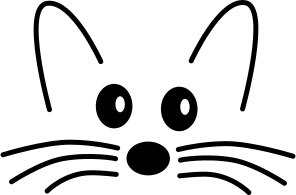
\includegraphics[width=1.4em]{squeak-logo}}}
\iftoshelse{
	\usepackage{marginnote}
		\renewcommand*{\marginfont}{\footnotesize}
	\newcommand{\vartriangleout}{\ifthenelse{\isodd{\thepage}}{\vartriangleright}{\vartriangleleft}}
	\newcommand{\dothisicon}{\fcolorbox{blue!65}{white}{\highlight{$\vartriangleout$}}}
	\newcommand{\dothis}[1]{%
		\noindent\par\noindent
		{\reversemarginpar
			\marginnote{\fcolorbox{blue!65}{white}{\highlight{$\vartriangleout$}}}}
		%\MarginLabel{do this}
		\noindent\emph{#1}
		\nopagebreak}
}{
	\newcommand{\dothisicon}{\raisebox{-.5ex}{
\includegraphics[height=1.2em]{pharo}}}
	\newcommand{\dothis}[1]{%
		\medskip
		\noindent\dothisicon
		\ifx#1\empty\else\quad\emph{#1}\fi
		\par\smallskip\nopagebreak}
}
%===> NEW VERSION <===
% NB: To use this in an individual chapter, you must set:
%\graphicspath{{figures/} {../figures/}}
% at the head of the chapter.  Don't forget the final /
%=============================================================
%:Reader hints (hint)
%
% Indicates a non-obvious consequence 
\newcommand{\hint}[1]{\vspace{1ex}\noindent\fbox{\textsc{Hint}} \emph{#1}}
%=================================================================
% graphics for Morphic handles
\newcommand{\grabHandle}{\raisebox{-0.2ex}{
\includegraphics[width=1em]{blackHandle}}}
\newcommand{\moveHandle}{\raisebox{-0.2ex}{
\includegraphics[width=1em]{moveHandle}}}
\newcommand{\debugHandle}{\raisebox{-0.2ex}{
\includegraphics[width=1em]{debugHandle}}}
%=============================================================
%:Highlighting Important stuff (doublebox)
%
% From Seaside book ...
\newsavebox{\SavedText}
\newlength{\InnerBoxRule}\setlength{\InnerBoxRule}{.75\fboxrule}
\newlength{\OuterBoxRule}\setlength{\OuterBoxRule}{1.5\fboxrule}
\newlength{\BoxSeparation}\setlength{\BoxSeparation}{1.5\fboxrule}
\addtolength{\BoxSeparation}{.5pt}
\newlength{\SaveBoxSep}\setlength{\SaveBoxSep}{2\fboxsep}
%
\newenvironment{doublebox}{\begin{lrbox}{\SavedText}
    \begin{minipage}{.75\textwidth}}
    {\end{minipage}\end{lrbox}\begin{center}
    \setlength{\fboxsep}{\BoxSeparation}\setlength{\fboxrule}{\OuterBoxRule}
    \fbox{\setlength{\fboxsep}{\SaveBoxSep}\setlength{\fboxrule}{\InnerBoxRule}%
      \fbox{\usebox{\SavedText}}}
  \end{center}}
% Use this:
\newcommand{\important}[1]{\begin{doublebox}#1\end{doublebox}}
%=============================================================
%:Section depth
\setcounter{secnumdepth}{2}
%% for this to happen start the file with
%\ifx\wholebook\relax\else
%% $Author$
% $Date$
% $Revision$

% HISTORY:
% 2006-10-31 - Oscar code macros
% ...

%=============================================================
% NB: documentclass must be set in main document.
% Allows book to be generated in multiple formats.
%=============================================================
%:Packages
\usepackage[T1]{fontenc}  %%%%%% really important to get the code directly in the text!
\usepackage{lmodern}
%\usepackage[scaled=0.85]{bookmanx} % needs another scale factor if used with \renewcommand{\sfdefault}{cmbr}
\usepackage{palatino}
\usepackage[scaled=0.85]{helvet}
\usepackage[protrusion,expansion=false]{microtype}
\usepackage{graphicx}
\usepackage{theorem}
\usepackage[english]{babel}
% ON: pdfsync breaks the use of p{width} for tabular columns!
\ifdefined\usepdfsync\usepackage{pdfsync}\fi % Requires texlive 2007
%=============================================================
%:More packages
%Stef should check which ones are used!
%\usepackage{picinpar}
%\usepackage{layout}
%\usepackage{color}
%\usepackage{enum}
%\usepackage{a4wide}
% \usepackage{fancyhdr}
\usepackage{ifthen}
\usepackage{float}
\usepackage{longtable}
\usepackage{makeidx}
\usepackage[nottoc]{tocbibind}
\usepackage{multicol}
\usepackage{booktabs}	% book-style tables
\usepackage{topcapt}	% enables \topcaption
\usepackage{multirow}
\usepackage{tabularx}
%\usepackage[bottom]{footmisc}
\usepackage{xspace}
\usepackage{alltt}
\usepackage{amssymb,textcomp}
\usepackage[usenames,dvipsnames]{color}
%\usepackage{colortbl}
\usepackage[hang]{subfigure}\makeatletter\def\p@subfigure{\thefigure\,}\makeatother
\usepackage{rotating}
\usepackage{enumitem}	% apb: allows more control over tags in enumerations
\usepackage{verbatim}     % for comment environment
\usepackage{varioref}	% for page references that work
\labelformat{footnote}{\thechapter--#1} % to distinguish citations from jurabib
\usepackage{needspace}
\usepackage{isodateo} % enable \isodate
\usepackage[newparttoc]{titlesec}
\usepackage{titletoc}
\usepackage{wrapfig}
\usepackage[
	super,
	citefull=first,
	authorformat={allreversed,and},
	titleformat={commasep,italic}
]{jurabib} % citations as footnotes
\usepackage[
	colorlinks=true,
	linkcolor=black,
	urlcolor=black,
	citecolor=black
]{hyperref}   % should come last
%=============================================================
%:PDF version
\pdfminorversion=3 % Set PDF to 1.3 for Lulu
%=============================================================
%:URL style
\makeatletter
\def\url@leostyle{%
  \@ifundefined{selectfont}{\def\UrlFont{\sf}}{\def\UrlFont{\sffamily}}}
\makeatother
% Now actually use the newly defined style.
\urlstyle{leo}
%=============================================================
%:Booleans
\newboolean{lulu}
\setboolean{lulu}{false}
\newcommand{\ifluluelse}[2]{\ifthenelse{\boolean{lulu}}{#1}{#2}}
%=============================================================
%:Names
\newcommand{\SUnit}{SUnit\xspace}
\newcommand{\sunit}{SUnit\xspace}
\newcommand{\xUnit}{$x$Unit\xspace}
\newcommand{\JUnit}{JUnit\xspace}
\newcommand{\st}{Smalltalk\xspace}
\newcommand{\pharo}{Pharo\xspace} % Use this, not \Pharo
%\newcommand{\sqmap}{SqueakMap\xspace}
\newcommand{\squeak}{Squeak\xspace} % use this, not \Squeak or \sq
\newcommand{\sqsrc}{SqueakSource\xspace}
\newcommand{\sbe}{\url{http://SqueakByExample.org}\xspace}
\newcommand{\pharoweb}{\url{http://pharo-project.org}\xspace}
\newcommand{\pbe}{\url{http://PharoByExample.org}\xspace}
\newcommand{\sba}{\url{http://SquareBracketAssociates.org}\xspace}
\newcommand{\bam}{\lct{Bounc\-ing\-Atoms\-Morph}\xspace}
%=============================================================
%:Markup macros for proof-reading
\usepackage[normalem]{ulem} % for \sout
\usepackage{xcolor}
\newcommand{\ra}{$\rightarrow$}
\newcommand{\ugh}[1]{\textcolor{red}{\uwave{#1}}} % please rephrase
\newcommand{\ins}[1]{\textcolor{blue}{\uline{#1}}} % please insert
\newcommand{\del}[1]{\textcolor{red}{\sout{#1}}} % please delete
\newcommand{\chg}[2]{\textcolor{red}{\sout{#1}}{\ra}\textcolor{blue}{\uline{#2}}} % please change
%=============================================================
%:Editorial comment macros
%\newcommand{\nnbb}[2]{
%    % \fbox{\bfseries\sffamily\scriptsize#1}
%    \fcolorbox{gray}{yellow}{\bfseries\sffamily\scriptsize#1}
%    {\sf\small$\blacktriangleright$\textit{#2}$\blacktriangleleft$}
%   }
\newcommand{\yellowbox}[1]{\fcolorbox{gray}{yellow}{\bfseries\sffamily\scriptsize#1}}
\newcommand{\triangles}[1]{{\sf\small$\blacktriangleright$\textit{#1}$\blacktriangleleft$}}
\newcommand{\nnbb}[2]{\yellowbox{#1} \triangles{#2}}
\newcommand{\fix}{\yellowbox{FIX!}}
\newcommand{\here}{\yellowbox{CONTINUE HERE!}}
% editor macros
\newcommand{\apl}[1]{\nnbb{Alain}{#1}} % Alain
\newcommand{\ab}[1]{\nnbb{Andrew}{#1}} % Black
\newcommand{\sd}[1]{\nnbb{St\'{e}f}{#1}} % Ducasse
\newcommand{\dc}[1]{\nnbb{DamienC}{#1}} % Ducasse
\newcommand{\md}[1]{\nnbb{Marcus}{#1}} % Denker
\newcommand{\on}[1]{\nnbb{Oscar}{#1}} % Nierstrasz
\newcommand{\damien}[1]{\nnbb{Damien}{#1}} % Pollet
\newcommand{\lr}[1]{\nnbb{Lukas}{#1}} % Renggli
\newcommand{\orla}[1]{\nnbb{Orla}{#1}} % Greevy
\newcommand{\alex}[1]{\nnbb{Alex}{#1}} % Bergel
\newcommand{\alx}[1]{\nnbb{Alex}{#1}} % Bergel
\newcommand{\dr}[1]{\nnbb{David}{#1}} % Roethlisberger
\newcommand{\ja}[1]{\nnbb{Jannik}{#1}} % Laval
\newcommand{\jr}[1]{\nnbb{Jorge}{#1}} % Ressia
\newcommand{\jb}[1]{\nnbb{JB}{#1}} % JB
\newcommand{\fp}[1]{\nnbb{Fabrizio}{#1}} % Perin
\newcommand{\michael}[1]{\nnbb{Michael}{#1}} % Davies
\newcommand{\ew}[1]{\nnbb{Erwann}{#1}} % Wernli
\newcommand{\mb}[1]{\nnbb{Martial}{#1}} % Boniou
\newcommand{\hw}[1]{\nnbb{Hernan}{#1}} % Wilkinson
\newcommand{\ben}[1]{\nnbb{Benjamin}{#1}} % Benjamin Van Ryseghem
%=============================================================
%:Abbreviation macros
\newcommand{\ie}{\emph{i.e.},\xspace}
\newcommand{\eg}{\emph{e.g.},\xspace}
\newcommand{\etc}{etc.\xspace}
%=============================================================
%:Cross reference macros
\newcommand{\charef}[1]{Chapter~\ref{cha:#1}\xspace}
\newcommand{\secref}[1]{Section~\ref{sec:#1}\xspace}
\newcommand{\figref}[1]{Figure~\ref{fig:#1}\xspace}
\newcommand{\Figref}[1]{Figure~\ref{fig:#1}\xspace}
\newcommand{\appref}[1]{Appendix~\ref{app:#1}\xspace}
\newcommand{\tabref}[1]{Table~\ref{tab:#1}\xspace}
\newcommand{\faqref}[1]{FAQ~\ref{faq:#1}, p.~\pageref{faq:#1}\xspace}
% APB: I removed trailing \xspace commands from these macros because
% \xspace mostly doesn't work.  If you want a space after your
% references, type one!
% ON: xspace has always worked just fine for me!  Please leave them in.
%
\newcommand{\ruleref}[1]{\ref{rule:#1}\xspace}
%
\newcommand{\egref}[1]{example~\ref{eg:#1}\xspace}
\newcommand{\Egref}[1]{Example~\ref{eg:#1}\xspace}
%
\newcommand{\scrref}[1]{script~\ref{scr:#1}\xspace}
\newcommand{\Scrref}[1]{Script~\ref{scr:#1}\xspace}
\newcommand{\tscrref}[1]{the script~\ref{scr:#1}\xspace}
\newcommand{\Tscrref}[1]{The script~\ref{scr:#1}\xspace}
%
\newcommand{\mthref}[1]{method~\ref{mth:#1}\xspace}
\newcommand{\mthsref}[1]{methods~\ref{mth:#1}\xspace}
\newcommand{\Mthref}[1]{Method~\ref{mth:#1}\xspace}
\newcommand{\tmthref}[1]{the method~\ref{mth:#1}\xspace}
\newcommand{\Tmthref}[1]{The method~\ref{mth:#1}\xspace}
%
\newcommand{\clsref}[1]{class~\ref{cls:#1}\xspace}
\newcommand{\tclsref}[1]{the class~\ref{cls:#1}\xspace}
\newcommand{\Tclsref}[1]{The class~\ref{cls:#1}\xspace}

\newcommand{\chalabel}[1]{\label{cha:#1}}
\newcommand{\seclabel}[1]{\label{sec:#1}}
\newcommand{\figlabel}[1]{\label{fig:#1}}
\newcommand{\tablabel}[1]{\label{tab:#1}}
\newcommand{\rulelabel}[1]{\label{rule:#1}}
\newcommand{\eglabel}[1]{\label{eg:#1}}
\newcommand{\scrlabel}[1]{\label{scr:#1}}
\newcommand{\mthlabel}[1]{\label{mth:#1}}
\newcommand{\clslabel}[1]{\label{cls:#1}}
\newcommand{\faqlabel}[1]{\label{faq:#1}}
%=============================================================
%:Menu item macro
% for menu items, so we can change our minds on how to print them! (apb)
\definecolor{lightgray}{gray}{0.89}
\newcommand{\menu}[1]{{%
	\setlength{\fboxsep}{0pt}%
	\colorbox{lightgray}{{{\upshape\sffamily\strut \,#1\,}}}}}
\newcommand{\link}[1]{{%
	\fontfamily{lmr}\selectfont
 	\upshape{\sffamily \underline{#1}}}}
% For submenu items:
\newcommand{\go}{\,$\triangleright$\,}
% \newcommand{\go}{\,$\blacktriangleright$\,}
% For keyboard shortcuts:
%\newcommand{\short}[1]{\mbox{$\langle${\sc CMD}$\rangle$-#1}\xspace}
\newcommand{\short}[1]{\mbox{{\sc cmd}\hspace{0.08em}--\hspace{0.09em}#1}\xspace}
% For buttons:
\newcommand{\button}[1]{{%
	\setlength{\fboxsep}{0pt}%
	\fbox{{\upshape\sffamily\strut \,#1\,}}}}
% NB: The button macro does not work within captions -- incompatible with xcolor package :-(
\newcommand{\toolsflap}{\textit{Tools} flap\xspace}
%=============================================================
%:Mouse clicks
\newcommand{\click}{click\xspace} % RED
\newcommand{\actclick}{action-click\xspace} % YELLOW
\newcommand{\metaclick}{meta-click\xspace} % BLUE
\newcommand{\Click}{Click\xspace} % RED
\newcommand{\Actclick}{Action-click\xspace} % YELLOW
\newcommand{\Metaclick}{Meta-click\xspace} % BLUE
%=============================================================
%:ToSh macros
\newboolean{tosh}
\setboolean{tosh}{false}
\newcommand{\iftoshelse}[2]{\ifthenelse{\boolean{tosh}}{#1}{#2}}
%=============================================================
%:ToSh colors
%\newcommand{\highlightcolor}{\color{blue!65}}
%\newcommand{\boxcolor}{\color{gray!25}}
\newcommand{\highlight}[1]{\textcolor{blue!65}{#1}}
%\newcommand{\codecolor}{\color{blue!65}}
%%\setlength{\fboxrule}{2pt}
%\newcommand{\asPict}[1]{%
%	{\Large\highlight{#1}}}
%=============================================================
%:Reader cues (do this)
%
% Indicate something the reader should try out.
% \newcommand{\dothisicon}{\raisebox{-.5ex}{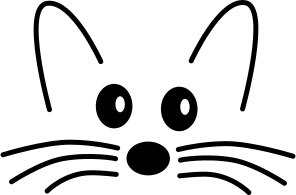
\includegraphics[width=1.4em]{squeak-logo}}}
\iftoshelse{
	\usepackage{marginnote}
		\renewcommand*{\marginfont}{\footnotesize}
	\newcommand{\vartriangleout}{\ifthenelse{\isodd{\thepage}}{\vartriangleright}{\vartriangleleft}}
	\newcommand{\dothisicon}{\fcolorbox{blue!65}{white}{\highlight{$\vartriangleout$}}}
	\newcommand{\dothis}[1]{%
		\noindent\par\noindent
		{\reversemarginpar
			\marginnote{\fcolorbox{blue!65}{white}{\highlight{$\vartriangleout$}}}}
		%\MarginLabel{do this}
		\noindent\emph{#1}
		\nopagebreak}
}{
	\newcommand{\dothisicon}{\raisebox{-.5ex}{
\includegraphics[height=1.2em]{pharo}}}
	\newcommand{\dothis}[1]{%
		\medskip
		\noindent\dothisicon
		\ifx#1\empty\else\quad\emph{#1}\fi
		\par\smallskip\nopagebreak}
}
%===> NEW VERSION <===
% NB: To use this in an individual chapter, you must set:
%\graphicspath{{figures/} {../figures/}}
% at the head of the chapter.  Don't forget the final /
%=============================================================
%:Reader hints (hint)
%
% Indicates a non-obvious consequence 
\newcommand{\hint}[1]{\vspace{1ex}\noindent\fbox{\textsc{Hint}} \emph{#1}}
%=================================================================
% graphics for Morphic handles
\newcommand{\grabHandle}{\raisebox{-0.2ex}{
\includegraphics[width=1em]{blackHandle}}}
\newcommand{\moveHandle}{\raisebox{-0.2ex}{
\includegraphics[width=1em]{moveHandle}}}
\newcommand{\debugHandle}{\raisebox{-0.2ex}{
\includegraphics[width=1em]{debugHandle}}}
%=============================================================
%:Highlighting Important stuff (doublebox)
%
% From Seaside book ...
\newsavebox{\SavedText}
\newlength{\InnerBoxRule}\setlength{\InnerBoxRule}{.75\fboxrule}
\newlength{\OuterBoxRule}\setlength{\OuterBoxRule}{1.5\fboxrule}
\newlength{\BoxSeparation}\setlength{\BoxSeparation}{1.5\fboxrule}
\addtolength{\BoxSeparation}{.5pt}
\newlength{\SaveBoxSep}\setlength{\SaveBoxSep}{2\fboxsep}
%
\newenvironment{doublebox}{\begin{lrbox}{\SavedText}
    \begin{minipage}{.75\textwidth}}
    {\end{minipage}\end{lrbox}\begin{center}
    \setlength{\fboxsep}{\BoxSeparation}\setlength{\fboxrule}{\OuterBoxRule}
    \fbox{\setlength{\fboxsep}{\SaveBoxSep}\setlength{\fboxrule}{\InnerBoxRule}%
      \fbox{\usebox{\SavedText}}}
  \end{center}}
% Use this:
\newcommand{\important}[1]{\begin{doublebox}#1\end{doublebox}}
%=============================================================
%:Section depth
\setcounter{secnumdepth}{2}
%% for this to happen start the file with
%\ifx\wholebook\relax\else
%% $Author$
% $Date$
% $Revision$

% HISTORY:
% 2006-10-31 - Oscar code macros
% ...

%=============================================================
% NB: documentclass must be set in main document.
% Allows book to be generated in multiple formats.
%=============================================================
%:Packages
\usepackage[T1]{fontenc}  %%%%%% really important to get the code directly in the text!
\usepackage{lmodern}
%\usepackage[scaled=0.85]{bookmanx} % needs another scale factor if used with \renewcommand{\sfdefault}{cmbr}
\usepackage{palatino}
\usepackage[scaled=0.85]{helvet}
\usepackage[protrusion,expansion=false]{microtype}
\usepackage{graphicx}
\usepackage{theorem}
\usepackage[english]{babel}
% ON: pdfsync breaks the use of p{width} for tabular columns!
\ifdefined\usepdfsync\usepackage{pdfsync}\fi % Requires texlive 2007
%=============================================================
%:More packages
%Stef should check which ones are used!
%\usepackage{picinpar}
%\usepackage{layout}
%\usepackage{color}
%\usepackage{enum}
%\usepackage{a4wide}
% \usepackage{fancyhdr}
\usepackage{ifthen}
\usepackage{float}
\usepackage{longtable}
\usepackage{makeidx}
\usepackage[nottoc]{tocbibind}
\usepackage{multicol}
\usepackage{booktabs}	% book-style tables
\usepackage{topcapt}	% enables \topcaption
\usepackage{multirow}
\usepackage{tabularx}
%\usepackage[bottom]{footmisc}
\usepackage{xspace}
\usepackage{alltt}
\usepackage{amssymb,textcomp}
\usepackage[usenames,dvipsnames]{color}
%\usepackage{colortbl}
\usepackage[hang]{subfigure}\makeatletter\def\p@subfigure{\thefigure\,}\makeatother
\usepackage{rotating}
\usepackage{enumitem}	% apb: allows more control over tags in enumerations
\usepackage{verbatim}     % for comment environment
\usepackage{varioref}	% for page references that work
\labelformat{footnote}{\thechapter--#1} % to distinguish citations from jurabib
\usepackage{needspace}
\usepackage{isodateo} % enable \isodate
\usepackage[newparttoc]{titlesec}
\usepackage{titletoc}
\usepackage{wrapfig}
\usepackage[
	super,
	citefull=first,
	authorformat={allreversed,and},
	titleformat={commasep,italic}
]{jurabib} % citations as footnotes
\usepackage[
	colorlinks=true,
	linkcolor=black,
	urlcolor=black,
	citecolor=black
]{hyperref}   % should come last
%=============================================================
%:PDF version
\pdfminorversion=3 % Set PDF to 1.3 for Lulu
%=============================================================
%:URL style
\makeatletter
\def\url@leostyle{%
  \@ifundefined{selectfont}{\def\UrlFont{\sf}}{\def\UrlFont{\sffamily}}}
\makeatother
% Now actually use the newly defined style.
\urlstyle{leo}
%=============================================================
%:Booleans
\newboolean{lulu}
\setboolean{lulu}{false}
\newcommand{\ifluluelse}[2]{\ifthenelse{\boolean{lulu}}{#1}{#2}}
%=============================================================
%:Names
\newcommand{\SUnit}{SUnit\xspace}
\newcommand{\sunit}{SUnit\xspace}
\newcommand{\xUnit}{$x$Unit\xspace}
\newcommand{\JUnit}{JUnit\xspace}
\newcommand{\st}{Smalltalk\xspace}
\newcommand{\pharo}{Pharo\xspace} % Use this, not \Pharo
%\newcommand{\sqmap}{SqueakMap\xspace}
\newcommand{\squeak}{Squeak\xspace} % use this, not \Squeak or \sq
\newcommand{\sqsrc}{SqueakSource\xspace}
\newcommand{\sbe}{\url{http://SqueakByExample.org}\xspace}
\newcommand{\pharoweb}{\url{http://pharo-project.org}\xspace}
\newcommand{\pbe}{\url{http://PharoByExample.org}\xspace}
\newcommand{\sba}{\url{http://SquareBracketAssociates.org}\xspace}
\newcommand{\bam}{\lct{Bounc\-ing\-Atoms\-Morph}\xspace}
%=============================================================
%:Markup macros for proof-reading
\usepackage[normalem]{ulem} % for \sout
\usepackage{xcolor}
\newcommand{\ra}{$\rightarrow$}
\newcommand{\ugh}[1]{\textcolor{red}{\uwave{#1}}} % please rephrase
\newcommand{\ins}[1]{\textcolor{blue}{\uline{#1}}} % please insert
\newcommand{\del}[1]{\textcolor{red}{\sout{#1}}} % please delete
\newcommand{\chg}[2]{\textcolor{red}{\sout{#1}}{\ra}\textcolor{blue}{\uline{#2}}} % please change
%=============================================================
%:Editorial comment macros
%\newcommand{\nnbb}[2]{
%    % \fbox{\bfseries\sffamily\scriptsize#1}
%    \fcolorbox{gray}{yellow}{\bfseries\sffamily\scriptsize#1}
%    {\sf\small$\blacktriangleright$\textit{#2}$\blacktriangleleft$}
%   }
\newcommand{\yellowbox}[1]{\fcolorbox{gray}{yellow}{\bfseries\sffamily\scriptsize#1}}
\newcommand{\triangles}[1]{{\sf\small$\blacktriangleright$\textit{#1}$\blacktriangleleft$}}
\newcommand{\nnbb}[2]{\yellowbox{#1} \triangles{#2}}
\newcommand{\fix}{\yellowbox{FIX!}}
\newcommand{\here}{\yellowbox{CONTINUE HERE!}}
% editor macros
\newcommand{\apl}[1]{\nnbb{Alain}{#1}} % Alain
\newcommand{\ab}[1]{\nnbb{Andrew}{#1}} % Black
\newcommand{\sd}[1]{\nnbb{St\'{e}f}{#1}} % Ducasse
\newcommand{\dc}[1]{\nnbb{DamienC}{#1}} % Ducasse
\newcommand{\md}[1]{\nnbb{Marcus}{#1}} % Denker
\newcommand{\on}[1]{\nnbb{Oscar}{#1}} % Nierstrasz
\newcommand{\damien}[1]{\nnbb{Damien}{#1}} % Pollet
\newcommand{\lr}[1]{\nnbb{Lukas}{#1}} % Renggli
\newcommand{\orla}[1]{\nnbb{Orla}{#1}} % Greevy
\newcommand{\alex}[1]{\nnbb{Alex}{#1}} % Bergel
\newcommand{\alx}[1]{\nnbb{Alex}{#1}} % Bergel
\newcommand{\dr}[1]{\nnbb{David}{#1}} % Roethlisberger
\newcommand{\ja}[1]{\nnbb{Jannik}{#1}} % Laval
\newcommand{\jr}[1]{\nnbb{Jorge}{#1}} % Ressia
\newcommand{\jb}[1]{\nnbb{JB}{#1}} % JB
\newcommand{\fp}[1]{\nnbb{Fabrizio}{#1}} % Perin
\newcommand{\michael}[1]{\nnbb{Michael}{#1}} % Davies
\newcommand{\ew}[1]{\nnbb{Erwann}{#1}} % Wernli
\newcommand{\mb}[1]{\nnbb{Martial}{#1}} % Boniou
\newcommand{\hw}[1]{\nnbb{Hernan}{#1}} % Wilkinson
\newcommand{\ben}[1]{\nnbb{Benjamin}{#1}} % Benjamin Van Ryseghem
%=============================================================
%:Abbreviation macros
\newcommand{\ie}{\emph{i.e.},\xspace}
\newcommand{\eg}{\emph{e.g.},\xspace}
\newcommand{\etc}{etc.\xspace}
%=============================================================
%:Cross reference macros
\newcommand{\charef}[1]{Chapter~\ref{cha:#1}\xspace}
\newcommand{\secref}[1]{Section~\ref{sec:#1}\xspace}
\newcommand{\figref}[1]{Figure~\ref{fig:#1}\xspace}
\newcommand{\Figref}[1]{Figure~\ref{fig:#1}\xspace}
\newcommand{\appref}[1]{Appendix~\ref{app:#1}\xspace}
\newcommand{\tabref}[1]{Table~\ref{tab:#1}\xspace}
\newcommand{\faqref}[1]{FAQ~\ref{faq:#1}, p.~\pageref{faq:#1}\xspace}
% APB: I removed trailing \xspace commands from these macros because
% \xspace mostly doesn't work.  If you want a space after your
% references, type one!
% ON: xspace has always worked just fine for me!  Please leave them in.
%
\newcommand{\ruleref}[1]{\ref{rule:#1}\xspace}
%
\newcommand{\egref}[1]{example~\ref{eg:#1}\xspace}
\newcommand{\Egref}[1]{Example~\ref{eg:#1}\xspace}
%
\newcommand{\scrref}[1]{script~\ref{scr:#1}\xspace}
\newcommand{\Scrref}[1]{Script~\ref{scr:#1}\xspace}
\newcommand{\tscrref}[1]{the script~\ref{scr:#1}\xspace}
\newcommand{\Tscrref}[1]{The script~\ref{scr:#1}\xspace}
%
\newcommand{\mthref}[1]{method~\ref{mth:#1}\xspace}
\newcommand{\mthsref}[1]{methods~\ref{mth:#1}\xspace}
\newcommand{\Mthref}[1]{Method~\ref{mth:#1}\xspace}
\newcommand{\tmthref}[1]{the method~\ref{mth:#1}\xspace}
\newcommand{\Tmthref}[1]{The method~\ref{mth:#1}\xspace}
%
\newcommand{\clsref}[1]{class~\ref{cls:#1}\xspace}
\newcommand{\tclsref}[1]{the class~\ref{cls:#1}\xspace}
\newcommand{\Tclsref}[1]{The class~\ref{cls:#1}\xspace}

\newcommand{\chalabel}[1]{\label{cha:#1}}
\newcommand{\seclabel}[1]{\label{sec:#1}}
\newcommand{\figlabel}[1]{\label{fig:#1}}
\newcommand{\tablabel}[1]{\label{tab:#1}}
\newcommand{\rulelabel}[1]{\label{rule:#1}}
\newcommand{\eglabel}[1]{\label{eg:#1}}
\newcommand{\scrlabel}[1]{\label{scr:#1}}
\newcommand{\mthlabel}[1]{\label{mth:#1}}
\newcommand{\clslabel}[1]{\label{cls:#1}}
\newcommand{\faqlabel}[1]{\label{faq:#1}}
%=============================================================
%:Menu item macro
% for menu items, so we can change our minds on how to print them! (apb)
\definecolor{lightgray}{gray}{0.89}
\newcommand{\menu}[1]{{%
	\setlength{\fboxsep}{0pt}%
	\colorbox{lightgray}{{{\upshape\sffamily\strut \,#1\,}}}}}
\newcommand{\link}[1]{{%
	\fontfamily{lmr}\selectfont
 	\upshape{\sffamily \underline{#1}}}}
% For submenu items:
\newcommand{\go}{\,$\triangleright$\,}
% \newcommand{\go}{\,$\blacktriangleright$\,}
% For keyboard shortcuts:
%\newcommand{\short}[1]{\mbox{$\langle${\sc CMD}$\rangle$-#1}\xspace}
\newcommand{\short}[1]{\mbox{{\sc cmd}\hspace{0.08em}--\hspace{0.09em}#1}\xspace}
% For buttons:
\newcommand{\button}[1]{{%
	\setlength{\fboxsep}{0pt}%
	\fbox{{\upshape\sffamily\strut \,#1\,}}}}
% NB: The button macro does not work within captions -- incompatible with xcolor package :-(
\newcommand{\toolsflap}{\textit{Tools} flap\xspace}
%=============================================================
%:Mouse clicks
\newcommand{\click}{click\xspace} % RED
\newcommand{\actclick}{action-click\xspace} % YELLOW
\newcommand{\metaclick}{meta-click\xspace} % BLUE
\newcommand{\Click}{Click\xspace} % RED
\newcommand{\Actclick}{Action-click\xspace} % YELLOW
\newcommand{\Metaclick}{Meta-click\xspace} % BLUE
%=============================================================
%:ToSh macros
\newboolean{tosh}
\setboolean{tosh}{false}
\newcommand{\iftoshelse}[2]{\ifthenelse{\boolean{tosh}}{#1}{#2}}
%=============================================================
%:ToSh colors
%\newcommand{\highlightcolor}{\color{blue!65}}
%\newcommand{\boxcolor}{\color{gray!25}}
\newcommand{\highlight}[1]{\textcolor{blue!65}{#1}}
%\newcommand{\codecolor}{\color{blue!65}}
%%\setlength{\fboxrule}{2pt}
%\newcommand{\asPict}[1]{%
%	{\Large\highlight{#1}}}
%=============================================================
%:Reader cues (do this)
%
% Indicate something the reader should try out.
% \newcommand{\dothisicon}{\raisebox{-.5ex}{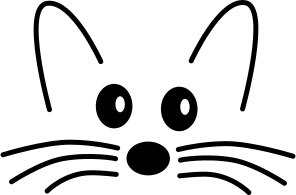
\includegraphics[width=1.4em]{squeak-logo}}}
\iftoshelse{
	\usepackage{marginnote}
		\renewcommand*{\marginfont}{\footnotesize}
	\newcommand{\vartriangleout}{\ifthenelse{\isodd{\thepage}}{\vartriangleright}{\vartriangleleft}}
	\newcommand{\dothisicon}{\fcolorbox{blue!65}{white}{\highlight{$\vartriangleout$}}}
	\newcommand{\dothis}[1]{%
		\noindent\par\noindent
		{\reversemarginpar
			\marginnote{\fcolorbox{blue!65}{white}{\highlight{$\vartriangleout$}}}}
		%\MarginLabel{do this}
		\noindent\emph{#1}
		\nopagebreak}
}{
	\newcommand{\dothisicon}{\raisebox{-.5ex}{
\includegraphics[height=1.2em]{pharo}}}
	\newcommand{\dothis}[1]{%
		\medskip
		\noindent\dothisicon
		\ifx#1\empty\else\quad\emph{#1}\fi
		\par\smallskip\nopagebreak}
}
%===> NEW VERSION <===
% NB: To use this in an individual chapter, you must set:
%\graphicspath{{figures/} {../figures/}}
% at the head of the chapter.  Don't forget the final /
%=============================================================
%:Reader hints (hint)
%
% Indicates a non-obvious consequence 
\newcommand{\hint}[1]{\vspace{1ex}\noindent\fbox{\textsc{Hint}} \emph{#1}}
%=================================================================
% graphics for Morphic handles
\newcommand{\grabHandle}{\raisebox{-0.2ex}{
\includegraphics[width=1em]{blackHandle}}}
\newcommand{\moveHandle}{\raisebox{-0.2ex}{
\includegraphics[width=1em]{moveHandle}}}
\newcommand{\debugHandle}{\raisebox{-0.2ex}{
\includegraphics[width=1em]{debugHandle}}}
%=============================================================
%:Highlighting Important stuff (doublebox)
%
% From Seaside book ...
\newsavebox{\SavedText}
\newlength{\InnerBoxRule}\setlength{\InnerBoxRule}{.75\fboxrule}
\newlength{\OuterBoxRule}\setlength{\OuterBoxRule}{1.5\fboxrule}
\newlength{\BoxSeparation}\setlength{\BoxSeparation}{1.5\fboxrule}
\addtolength{\BoxSeparation}{.5pt}
\newlength{\SaveBoxSep}\setlength{\SaveBoxSep}{2\fboxsep}
%
\newenvironment{doublebox}{\begin{lrbox}{\SavedText}
    \begin{minipage}{.75\textwidth}}
    {\end{minipage}\end{lrbox}\begin{center}
    \setlength{\fboxsep}{\BoxSeparation}\setlength{\fboxrule}{\OuterBoxRule}
    \fbox{\setlength{\fboxsep}{\SaveBoxSep}\setlength{\fboxrule}{\InnerBoxRule}%
      \fbox{\usebox{\SavedText}}}
  \end{center}}
% Use this:
\newcommand{\important}[1]{\begin{doublebox}#1\end{doublebox}}
%=============================================================
%:Section depth
\setcounter{secnumdepth}{2}
%% for this to happen start the file with
%\ifx\wholebook\relax\else
%\input{../common.tex}
%\begin{document}
%\fi
% and terminate by
% \ifx\wholebook\relax\else\end{document}\fi

\DeclareGraphicsExtensions{.pdf, .jpg, .png}
%=============================================================
%:PDF setup
\hypersetup{
%   a4paper,
%   pdfstartview=FitV,
%   colorlinks,
%   linkcolor=darkblue,
%   citecolor=darkblue,
   pdftitle={Pharo by Example},
   pdfauthor={Andrew P. Black, St\'ephane Ducasse,	Oscar Nierstrasz,
Damien Pollet},
   pdfkeywords={Smalltalk, Squeak, Object-Oriented Programming, OOP},
   pdfsubject={Computer Science}
}
%=============================================================
%:Page layout and appearance
%
% \renewcommand{\headrulewidth}{0pt}
\renewcommand{\chaptermark}[1]{\markboth{#1}{}}
\renewcommand{\sectionmark}[1]{\markright{\thesection\ #1}}
\renewpagestyle{plain}[\small\itshape]{%
	\setheadrule{0pt}%
	\sethead[][][]{}{}{}%
	\setfoot[][][]{}{}{}}
\renewpagestyle{headings}[\small\itshape]{%
	\setheadrule{0pt}%
	\setmarks{chapter}{section}%
	\sethead[\thepage][][\chaptertitle]{\sectiontitle}{}{\thepage}%
	\setfoot[][][]{}{}{}}
%=============================================================
%:Title section setup and TOC numbering depth
\setcounter{secnumdepth}{1}
\setcounter{tocdepth}{1}
\titleformat{\part}[display]{\centering}{\huge\partname\ \thepart}{1em}{\Huge\textbf}[]
\titleformat{\chapter}[display]{}{\huge\chaptertitlename\ \thechapter}{1em}{\Huge\raggedright\textbf}[]
\titlecontents{part}[3pc]{%
		\pagebreak[2]\addvspace{1em plus.4em minus.2em}%
		\leavevmode\large\bfseries}
	{\contentslabel{3pc}}{\hspace*{-3pc}}
	{}[\nopagebreak]
\titlecontents{chapter}[3pc]{%
		\pagebreak[0]\addvspace{1em plus.2em minus.2em}%
		\leavevmode\bfseries}
	{\contentslabel{3pc}}{}
	{\hfill\contentspage}[\nopagebreak]
\dottedcontents{section}[3pc]{}{3pc}{1pc}
\dottedcontents{subsection}[3pc]{}{0pc}{1pc}
% \dottedcontents{subsection}[4.5em]{}{0pt}{1pc}
% Make \cleardoublepage insert really blank pages http://www.tex.ac.uk/cgi-bin/texfaq2html?label=reallyblank
\let\origdoublepage\cleardoublepage
\newcommand{\clearemptydoublepage}{%
  \clearpage
  {\pagestyle{empty}\origdoublepage}}
\let\cleardoublepage\clearemptydoublepage % see http://www.tex.ac.uk/cgi-bin/texfaq2html?label=patch
%=============================================================
%:FAQ macros (for FAQ chapter)
\newtheorem{faq}{FAQ}
\newcommand{\answer}{\paragraph{Answer}\ }
%=============================================================
%:Listings package configuration
% \newcommand{\caret}{\makebox{\raisebox{0.4ex}{\footnotesize{$\wedge$}}}}
\newcommand{\caret}{\^\,}
\newcommand{\escape}{{\sf \textbackslash}}
\definecolor{source}{gray}{0.95}
\usepackage{listings}
\lstdefinelanguage{Smalltalk}{
%  morekeywords={self,super,true,false,nil,thisContext}, % This is overkill
  morestring=[d]',
  morecomment=[s]{"}{"},
  alsoletter={\#:},
  escapechar={!},
  literate=
    {BANG}{!}1
    {CARET}{\^}1
    {UNDERSCORE}{\_}1
    {\\st}{Smalltalk}9 % convenience -- in case \st occurs in code
    % {'}{{\textquotesingle}}1 % replaced by upquote=true in \lstset
    {_}{{$\leftarrow$}}1
    {>>>}{{\sep}}1
    {^}{{$\uparrow$}}1
    {~}{{$\sim$}}1
    {-}{{\texttt{-}}}1 %{\textminus}}1 %{-}{\hspace{-0.13em}}{-}}1  % the goal is to make - the same width as +
    % {+}{\sf+}1 %{\raisebox{0.08ex}{+}}}1      % and to raise + off the baseline to match -
    {-->}{{\quad$\longrightarrow$\quad}}3
	, % Don't forget the comma at the end!
  tabsize=4
}[keywords,comments,strings]

\lstset{language=Smalltalk,
	basicstyle=\sffamily,
	keywordstyle=\color{black}\bfseries,
	% stringstyle=\ttfamily, % Ugly! do we really want this? -- on
	mathescape=true,
	showstringspaces=false,
	keepspaces=true,
	breaklines=true,
	breakautoindent=true,
	backgroundcolor=\color{source},
	lineskip={-1pt}, % Ugly hack
	upquote=true, % straight quote; requires textcomp package
	columns=fullflexible} % no fixed width fonts
% In-line code (literal)
% Normally use this for all in-line code:
\newcommand{\ct}{\lstinline[mathescape=false,backgroundcolor=\color{white},basicstyle={\sffamily\upshape}]}
% apb 2007.8.28 added the \upshape declaration to avoid getting italicized code in \dothis{ } sections.
% In-line code (latex enabled)
% Use this only in special situations where \ct does not work
% (within section headings ...):
\newcommand{\lct}[1]{{\textsf{\textup{#1}}}}
% Use these for system categories and protocols:
\newcommand{\scat}[1]{\emph{\textsf{#1}}\xspace}
\newcommand{\pkg}[1]{\emph{\textsf{#1}}\xspace}
\newcommand{\prot}[1]{\emph{\textsf{#1}}\xspace}
% Code environments
% NB: the arg is for tests
% Only code and example environments may be tests
\lstnewenvironment{code}[1]{%
	\lstset{%
		% frame=lines,
		frame=single,
		framerule=0pt,
		mathescape=false
	}
}{}
\def\ignoredollar#1{}
%=============================================================
%:Code environments (method, script ...)
% NB: the third arg is for tests
% Only code and example environments may be tests
\lstnewenvironment{example}[3][defaultlabel]{%
	\renewcommand{\lstlistingname}{Example}%
	\lstset{
		% frame=lines,
		frame=single,
		framerule=0pt,
		mathescape=false,
		caption={\emph{#2}},
		label={eg:#1}
	}
}{}
\lstnewenvironment{script}[2][defaultlabel]{%
\renewcommand{\lstlistingname}{Script}%
	\lstset{
		% frame=lines,
		frame=single,
		framerule=0pt,
		mathescape=false,
		name={Script},
		caption={\emph{#2}},
		label={scr:#1}
	}
}{}
\lstnewenvironment{method}[2][defaultlabel]{%
	\renewcommand{\lstlistingname}{Method}%
	\lstset{
		% frame=lines,
		frame=single,
		framerule=0pt,
		mathescape=false,
		name={Method},
		caption={\emph{#2}},
		label={mth:#1}
	}
}{}
\lstnewenvironment{methods}[2][defaultlabel]{% just for multiple methods at once
	\renewcommand{\lstlistingname}{Methods}%
	\lstset{
		% frame=lines,
		frame=single,
		framerule=0pt,
		mathescape=false,
		name={Method},
		caption={\emph{#2}},
		label={mth:#1}
	}
}{}
\lstnewenvironment{numMethod}[2][defaultlabel]{%
	\renewcommand{\lstlistingname}{Method}%
	\lstset{
		numbers=left,
		numberstyle={\tiny\sffamily},
		% frame=lines,
		frame=single,
		framerule=0pt,
		mathescape=false,
		name={Method},
		caption={\emph{#2}},
		label={mth:#1}
	}
}{}
\lstnewenvironment{classdef}[2][defaultlabel]{%
	\renewcommand{\lstlistingname}{Class}%
	\lstset{
		% frame=lines,
		frame=single,
		framerule=0pt,
		mathescape=false,
		name={Class},
		caption={\emph{#2}},
		label={cls:#1}
	}
}{}
%=============================================================
%:Reserving space
% Usually need one more line than the actual lines of code
\newcommand{\needlines}[1]{\Needspace{#1\baselineskip}}
%=============================================================
%:Indexing macros
% Macros ending with "ind" generate text as well as an index entry
% Macros ending with "index" *only* generate an index entry
\newcommand{\ind}[1]{\index{#1}#1\xspace} % plain text
\newcommand{\subind}[2]{\index{#1!#2}#2\xspace} % show #2, subindex under #1
\newcommand{\emphind}[1]{\index{#1}\emph{#1}\xspace} % emph #1
\newcommand{\emphsubind}[2]{\index{#1!#2}\emph{#2}\xspace} % show emph #2, subindex inder #1
\newcommand{\scatind}[1]{\index{#1@\textsf{#1} (category)}\scat{#1}} % category
\newcommand{\pkgind}[1]{\index{#1@\textsf{#1} (package)}\pkg{#1}} % package
\newcommand{\protind}[1]{\index{#1@\textsf{#1} (protocol)}\prot{#1}} % protocol
\newcommand{\clsind}[1]{\index{#1@\textsf{#1} (class)}\ct{#1}\xspace}
% \newcommand{\clsind}[1]{\index{#1!\#@(class)}\ct{#1}\xspace} % class
\newcommand{\clsindplural}[1]{\index{#1!\#@(class)}\ct{#1}s\xspace} % class
\newcommand{\cvind}[1]{\index{#1@\textsf{#1} (class variable)}\ct{#1}\xspace} % class var
\newcommand{\glbind}[1]{\index{#1@\textsf{#1} (global)}\ct{#1}\xspace} % global
\newcommand{\patind}[1]{\index{#1@#1 (pattern)}\ct{#1}\xspace} % pattern
\newcommand{\pvind}[1]{\index{#1@\textsf{#1} (pseudo variable)}\ct{#1}\xspace} % pseudo var
\newcommand{\clsmthind}[2]{\index{#1!#2@\ct{#2}}\ct{#1>>>#2}\xspace} % class + method name
\newcommand{\mthind}[2]{\index{#1!#2@\ct{#2}}\ct{#2}\xspace} % show method name only
\newcommand{\lmthind}[2]{\index{#1!#2@\ct{#2}}\lct{#2}\xspace} % show method name only
\newcommand{\cmind}[2]{\index{#1!#2@\ct{#2}}\ct{#1>>>#2}\xspace} % show class>>method
\newcommand{\lcmind}[2]{\index{#1!#2@\ct{#2}}\lct{#1>>>#2}\xspace} % show class>>method
\newcommand{\toolsflapind}{\index{Tools flap}\toolsflap} % index tools flap
% The following only generate an index entry:
% \newcommand{\clsindex}[1]{\index{#1@\textsf{#1} (class)}}
\newcommand{\clsindex}[1]{\index{#1!\#@(class)}} % class
\newcommand{\mthindex}[2]{\index{#1!#2@\ct{#2}}} % method
\newcommand{\cmindex}[2]{\index{#1!#2@\ct{#2}}} % class>>method
\newcommand{\cvindex}[1]{\index{#1@\textsf{#1} (class variable)}} % class var
\newcommand{\glbindex}[1]{\index{#1@\textsf{#1} (global)}}% global
\newcommand{\pvindex}[1]{\index{#1@\textsf{#1} (pseudo variable)}}% pseudo var
\newcommand{\seeindex}[2]{\index{#1|see{#2}}} % #1, see #2
\newcommand{\scatindex}[1]{\index{#1@\textsf{#1} (category)}} % category
\newcommand{\pkgindex}[1]{\index{#1@\textsf{#1} (package)}} % package
\newcommand{\protindex}[1]{\index{#1@\textsf{#1} (protocol)}} % protocol
% How can we have the main entry page numbers in bold yet not break the hyperlink?
\newcommand{\boldidx}[1]{{\bf #1}} % breaks hyperlink
%\newcommand{\indmain}[1]{\index{#1|boldidx}#1\xspace} % plain text, main entry
%\newcommand{\emphsubindmain}[2]{\index{#1!#2|boldidx}\emph{#2}\xspace} % subindex, main entry
%\newcommand{\subindmain}[2]{\index{#1!#2|boldidx}#2\xspace} % subindex, main entry
%\newcommand{\clsindmain}[1]{\index{#1@\textsf{#1} (class)|boldidx}\ct{#1}\xspace}
%\newcommand{\clsindmain}[1]{\index{#1!\#@(class)|boldidx}\ct{#1}\xspace} % class main
%\newcommand{\indexmain}[1]{\index{#1|boldidx}} % main index entry only
\newcommand{\indmain}[1]{\index{#1}#1\xspace} % The main index entry for this item
\newcommand{\emphsubindmain}[2]{\index{#1!#2}\emph{#2}\xspace} % subindex, main entry
\newcommand{\subindmain}[2]{\index{#1!#2}#2\xspace} % subindex, main entry
%\newcommand{\clsindmain}[1]{\index{#1@\textsf{#1} (class)}\ct{#1}\xspace}
\newcommand{\clsindmain}[1]{\index{#1!\#@(class)}\ct{#1}\xspace} % class main
\newcommand{\clsindexmain}[1]{\index{#1!\#@(class)}} % class main index only
\newcommand{\indexmain}[1]{\index{#1}} 
%=============================================================
%:Code macros
% some constants
\newcommand{\codesize}{\small}
\newcommand{\codefont}{\sffamily}
%\newcommand{\cat}[1]{\textit{In category #1}}%%To remove later
\newlength{\scriptindent}
\setlength{\scriptindent}{.3cm}
%% Method presentation constants
\newlength{\methodindent}
\newlength{\methodwordlength}
\newlength{\aftermethod}
\setlength{\methodindent}{0.2cm}
\settowidth{\methodwordlength}{\ M\'ethode\ }
%=============================================================
%:Smalltalk macros
%\newcommand{\sep}{{$\gg$}}
\newcommand{\sep}{\mbox{>>}}
\newcommand{\self}{\lct{self}\xspace}
\newcommand{\super}{\lct{super}\xspace}
\newcommand{\nil}{\lct{nil}\xspace}
%=============================================================
% be less conservative about float placement
% these commands are from http://www.tex.ac.uk/cgi-bin/texfaq2html?label=floats
\renewcommand{\topfraction}{.9}
\renewcommand{\bottomfraction}{.9}
\renewcommand{\textfraction}{.1}
\renewcommand{\floatpagefraction}{.85}
\renewcommand{\dbltopfraction}{.66}
\renewcommand{\dblfloatpagefraction}{.85}
\setcounter{topnumber}{9}
\setcounter{bottomnumber}{9}
\setcounter{totalnumber}{20}
\setcounter{dbltopnumber}{9}
%=============================================================
% Give information from each chapter's author
\newcommand{\contact}[2]{\textbf{#1} \textsf{(#2)}}

\newcommand{\chapterauthor}[1]{\emph{with the participation of:\\#1}\\}

\newcommand{\authornoury}{\contact{Noury Bouraqadi}{bouraqadi@gmail.com}}
\newcommand{\authordamienc}{\contact{Damien Cassou}{damien.cassou@gmail.com}}
\newcommand{\authoroscar}{\contact{Oscar Nierstrasz}{oscar.nierstrasz@acm.org}}
\newcommand{\authorsteph}{\contact{St\'ephane Ducasse}{stephane.ducasse@inria.fr}}
\newcommand{\authoralex}{\contact{Alexandre Bergel}{alexandre@bergel.eu}}
\newcommand{\authorolivier}{\contact{Olivier Auverlot}{olivier.auverlot@inria.fr}}
\newcommand{\authornicolas}{\contact{Nicolas Cellier}{nicolas.cellier.aka.nice@gmail.com}}
\newcommand{\authormarcus}{\contact{Marcus Denker}{marcus.denker@inria.fr}}
\newcommand{\authoralain}{\contact{Alain Plantec}{alain.plantec@univ-brest.fr}}
\newcommand{\authordale}{\contact{Dale Henrichs}{dale.henrichs@gemstone.com}}
\newcommand{\authormariano}{\contact{Mariano Martinez Peck}{marianopeck@gmail.com}}
\newcommand{\authorsven}{\contact{Sven Van Caekenberghe}{sven@beta9.be}}
\newcommand{\authorlukas}{\contact{Lukas Renggli}{renggli@gmail.com}}

%=============================================================
% apb doesn't like paragraphs to run in to each other without a break
\parskip 1ex
%=============================================================
%:Stuff to check, merge or deprecate
%\setlength{\marginparsep}{2mm}
%\renewcommand{\baselinestretch}{1.1}
%=============================================================

%\begin{document}
%\fi
% and terminate by
% \ifx\wholebook\relax\else\end{document}\fi

\DeclareGraphicsExtensions{.pdf, .jpg, .png}
%=============================================================
%:PDF setup
\hypersetup{
%   a4paper,
%   pdfstartview=FitV,
%   colorlinks,
%   linkcolor=darkblue,
%   citecolor=darkblue,
   pdftitle={Pharo by Example},
   pdfauthor={Andrew P. Black, St\'ephane Ducasse,	Oscar Nierstrasz,
Damien Pollet},
   pdfkeywords={Smalltalk, Squeak, Object-Oriented Programming, OOP},
   pdfsubject={Computer Science}
}
%=============================================================
%:Page layout and appearance
%
% \renewcommand{\headrulewidth}{0pt}
\renewcommand{\chaptermark}[1]{\markboth{#1}{}}
\renewcommand{\sectionmark}[1]{\markright{\thesection\ #1}}
\renewpagestyle{plain}[\small\itshape]{%
	\setheadrule{0pt}%
	\sethead[][][]{}{}{}%
	\setfoot[][][]{}{}{}}
\renewpagestyle{headings}[\small\itshape]{%
	\setheadrule{0pt}%
	\setmarks{chapter}{section}%
	\sethead[\thepage][][\chaptertitle]{\sectiontitle}{}{\thepage}%
	\setfoot[][][]{}{}{}}
%=============================================================
%:Title section setup and TOC numbering depth
\setcounter{secnumdepth}{1}
\setcounter{tocdepth}{1}
\titleformat{\part}[display]{\centering}{\huge\partname\ \thepart}{1em}{\Huge\textbf}[]
\titleformat{\chapter}[display]{}{\huge\chaptertitlename\ \thechapter}{1em}{\Huge\raggedright\textbf}[]
\titlecontents{part}[3pc]{%
		\pagebreak[2]\addvspace{1em plus.4em minus.2em}%
		\leavevmode\large\bfseries}
	{\contentslabel{3pc}}{\hspace*{-3pc}}
	{}[\nopagebreak]
\titlecontents{chapter}[3pc]{%
		\pagebreak[0]\addvspace{1em plus.2em minus.2em}%
		\leavevmode\bfseries}
	{\contentslabel{3pc}}{}
	{\hfill\contentspage}[\nopagebreak]
\dottedcontents{section}[3pc]{}{3pc}{1pc}
\dottedcontents{subsection}[3pc]{}{0pc}{1pc}
% \dottedcontents{subsection}[4.5em]{}{0pt}{1pc}
% Make \cleardoublepage insert really blank pages http://www.tex.ac.uk/cgi-bin/texfaq2html?label=reallyblank
\let\origdoublepage\cleardoublepage
\newcommand{\clearemptydoublepage}{%
  \clearpage
  {\pagestyle{empty}\origdoublepage}}
\let\cleardoublepage\clearemptydoublepage % see http://www.tex.ac.uk/cgi-bin/texfaq2html?label=patch
%=============================================================
%:FAQ macros (for FAQ chapter)
\newtheorem{faq}{FAQ}
\newcommand{\answer}{\paragraph{Answer}\ }
%=============================================================
%:Listings package configuration
% \newcommand{\caret}{\makebox{\raisebox{0.4ex}{\footnotesize{$\wedge$}}}}
\newcommand{\caret}{\^\,}
\newcommand{\escape}{{\sf \textbackslash}}
\definecolor{source}{gray}{0.95}
\usepackage{listings}
\lstdefinelanguage{Smalltalk}{
%  morekeywords={self,super,true,false,nil,thisContext}, % This is overkill
  morestring=[d]',
  morecomment=[s]{"}{"},
  alsoletter={\#:},
  escapechar={!},
  literate=
    {BANG}{!}1
    {CARET}{\^}1
    {UNDERSCORE}{\_}1
    {\\st}{Smalltalk}9 % convenience -- in case \st occurs in code
    % {'}{{\textquotesingle}}1 % replaced by upquote=true in \lstset
    {_}{{$\leftarrow$}}1
    {>>>}{{\sep}}1
    {^}{{$\uparrow$}}1
    {~}{{$\sim$}}1
    {-}{{\texttt{-}}}1 %{\textminus}}1 %{-}{\hspace{-0.13em}}{-}}1  % the goal is to make - the same width as +
    % {+}{\sf+}1 %{\raisebox{0.08ex}{+}}}1      % and to raise + off the baseline to match -
    {-->}{{\quad$\longrightarrow$\quad}}3
	, % Don't forget the comma at the end!
  tabsize=4
}[keywords,comments,strings]

\lstset{language=Smalltalk,
	basicstyle=\sffamily,
	keywordstyle=\color{black}\bfseries,
	% stringstyle=\ttfamily, % Ugly! do we really want this? -- on
	mathescape=true,
	showstringspaces=false,
	keepspaces=true,
	breaklines=true,
	breakautoindent=true,
	backgroundcolor=\color{source},
	lineskip={-1pt}, % Ugly hack
	upquote=true, % straight quote; requires textcomp package
	columns=fullflexible} % no fixed width fonts
% In-line code (literal)
% Normally use this for all in-line code:
\newcommand{\ct}{\lstinline[mathescape=false,backgroundcolor=\color{white},basicstyle={\sffamily\upshape}]}
% apb 2007.8.28 added the \upshape declaration to avoid getting italicized code in \dothis{ } sections.
% In-line code (latex enabled)
% Use this only in special situations where \ct does not work
% (within section headings ...):
\newcommand{\lct}[1]{{\textsf{\textup{#1}}}}
% Use these for system categories and protocols:
\newcommand{\scat}[1]{\emph{\textsf{#1}}\xspace}
\newcommand{\pkg}[1]{\emph{\textsf{#1}}\xspace}
\newcommand{\prot}[1]{\emph{\textsf{#1}}\xspace}
% Code environments
% NB: the arg is for tests
% Only code and example environments may be tests
\lstnewenvironment{code}[1]{%
	\lstset{%
		% frame=lines,
		frame=single,
		framerule=0pt,
		mathescape=false
	}
}{}
\def\ignoredollar#1{}
%=============================================================
%:Code environments (method, script ...)
% NB: the third arg is for tests
% Only code and example environments may be tests
\lstnewenvironment{example}[3][defaultlabel]{%
	\renewcommand{\lstlistingname}{Example}%
	\lstset{
		% frame=lines,
		frame=single,
		framerule=0pt,
		mathescape=false,
		caption={\emph{#2}},
		label={eg:#1}
	}
}{}
\lstnewenvironment{script}[2][defaultlabel]{%
\renewcommand{\lstlistingname}{Script}%
	\lstset{
		% frame=lines,
		frame=single,
		framerule=0pt,
		mathescape=false,
		name={Script},
		caption={\emph{#2}},
		label={scr:#1}
	}
}{}
\lstnewenvironment{method}[2][defaultlabel]{%
	\renewcommand{\lstlistingname}{Method}%
	\lstset{
		% frame=lines,
		frame=single,
		framerule=0pt,
		mathescape=false,
		name={Method},
		caption={\emph{#2}},
		label={mth:#1}
	}
}{}
\lstnewenvironment{methods}[2][defaultlabel]{% just for multiple methods at once
	\renewcommand{\lstlistingname}{Methods}%
	\lstset{
		% frame=lines,
		frame=single,
		framerule=0pt,
		mathescape=false,
		name={Method},
		caption={\emph{#2}},
		label={mth:#1}
	}
}{}
\lstnewenvironment{numMethod}[2][defaultlabel]{%
	\renewcommand{\lstlistingname}{Method}%
	\lstset{
		numbers=left,
		numberstyle={\tiny\sffamily},
		% frame=lines,
		frame=single,
		framerule=0pt,
		mathescape=false,
		name={Method},
		caption={\emph{#2}},
		label={mth:#1}
	}
}{}
\lstnewenvironment{classdef}[2][defaultlabel]{%
	\renewcommand{\lstlistingname}{Class}%
	\lstset{
		% frame=lines,
		frame=single,
		framerule=0pt,
		mathescape=false,
		name={Class},
		caption={\emph{#2}},
		label={cls:#1}
	}
}{}
%=============================================================
%:Reserving space
% Usually need one more line than the actual lines of code
\newcommand{\needlines}[1]{\Needspace{#1\baselineskip}}
%=============================================================
%:Indexing macros
% Macros ending with "ind" generate text as well as an index entry
% Macros ending with "index" *only* generate an index entry
\newcommand{\ind}[1]{\index{#1}#1\xspace} % plain text
\newcommand{\subind}[2]{\index{#1!#2}#2\xspace} % show #2, subindex under #1
\newcommand{\emphind}[1]{\index{#1}\emph{#1}\xspace} % emph #1
\newcommand{\emphsubind}[2]{\index{#1!#2}\emph{#2}\xspace} % show emph #2, subindex inder #1
\newcommand{\scatind}[1]{\index{#1@\textsf{#1} (category)}\scat{#1}} % category
\newcommand{\pkgind}[1]{\index{#1@\textsf{#1} (package)}\pkg{#1}} % package
\newcommand{\protind}[1]{\index{#1@\textsf{#1} (protocol)}\prot{#1}} % protocol
\newcommand{\clsind}[1]{\index{#1@\textsf{#1} (class)}\ct{#1}\xspace}
% \newcommand{\clsind}[1]{\index{#1!\#@(class)}\ct{#1}\xspace} % class
\newcommand{\clsindplural}[1]{\index{#1!\#@(class)}\ct{#1}s\xspace} % class
\newcommand{\cvind}[1]{\index{#1@\textsf{#1} (class variable)}\ct{#1}\xspace} % class var
\newcommand{\glbind}[1]{\index{#1@\textsf{#1} (global)}\ct{#1}\xspace} % global
\newcommand{\patind}[1]{\index{#1@#1 (pattern)}\ct{#1}\xspace} % pattern
\newcommand{\pvind}[1]{\index{#1@\textsf{#1} (pseudo variable)}\ct{#1}\xspace} % pseudo var
\newcommand{\clsmthind}[2]{\index{#1!#2@\ct{#2}}\ct{#1>>>#2}\xspace} % class + method name
\newcommand{\mthind}[2]{\index{#1!#2@\ct{#2}}\ct{#2}\xspace} % show method name only
\newcommand{\lmthind}[2]{\index{#1!#2@\ct{#2}}\lct{#2}\xspace} % show method name only
\newcommand{\cmind}[2]{\index{#1!#2@\ct{#2}}\ct{#1>>>#2}\xspace} % show class>>method
\newcommand{\lcmind}[2]{\index{#1!#2@\ct{#2}}\lct{#1>>>#2}\xspace} % show class>>method
\newcommand{\toolsflapind}{\index{Tools flap}\toolsflap} % index tools flap
% The following only generate an index entry:
% \newcommand{\clsindex}[1]{\index{#1@\textsf{#1} (class)}}
\newcommand{\clsindex}[1]{\index{#1!\#@(class)}} % class
\newcommand{\mthindex}[2]{\index{#1!#2@\ct{#2}}} % method
\newcommand{\cmindex}[2]{\index{#1!#2@\ct{#2}}} % class>>method
\newcommand{\cvindex}[1]{\index{#1@\textsf{#1} (class variable)}} % class var
\newcommand{\glbindex}[1]{\index{#1@\textsf{#1} (global)}}% global
\newcommand{\pvindex}[1]{\index{#1@\textsf{#1} (pseudo variable)}}% pseudo var
\newcommand{\seeindex}[2]{\index{#1|see{#2}}} % #1, see #2
\newcommand{\scatindex}[1]{\index{#1@\textsf{#1} (category)}} % category
\newcommand{\pkgindex}[1]{\index{#1@\textsf{#1} (package)}} % package
\newcommand{\protindex}[1]{\index{#1@\textsf{#1} (protocol)}} % protocol
% How can we have the main entry page numbers in bold yet not break the hyperlink?
\newcommand{\boldidx}[1]{{\bf #1}} % breaks hyperlink
%\newcommand{\indmain}[1]{\index{#1|boldidx}#1\xspace} % plain text, main entry
%\newcommand{\emphsubindmain}[2]{\index{#1!#2|boldidx}\emph{#2}\xspace} % subindex, main entry
%\newcommand{\subindmain}[2]{\index{#1!#2|boldidx}#2\xspace} % subindex, main entry
%\newcommand{\clsindmain}[1]{\index{#1@\textsf{#1} (class)|boldidx}\ct{#1}\xspace}
%\newcommand{\clsindmain}[1]{\index{#1!\#@(class)|boldidx}\ct{#1}\xspace} % class main
%\newcommand{\indexmain}[1]{\index{#1|boldidx}} % main index entry only
\newcommand{\indmain}[1]{\index{#1}#1\xspace} % The main index entry for this item
\newcommand{\emphsubindmain}[2]{\index{#1!#2}\emph{#2}\xspace} % subindex, main entry
\newcommand{\subindmain}[2]{\index{#1!#2}#2\xspace} % subindex, main entry
%\newcommand{\clsindmain}[1]{\index{#1@\textsf{#1} (class)}\ct{#1}\xspace}
\newcommand{\clsindmain}[1]{\index{#1!\#@(class)}\ct{#1}\xspace} % class main
\newcommand{\clsindexmain}[1]{\index{#1!\#@(class)}} % class main index only
\newcommand{\indexmain}[1]{\index{#1}} 
%=============================================================
%:Code macros
% some constants
\newcommand{\codesize}{\small}
\newcommand{\codefont}{\sffamily}
%\newcommand{\cat}[1]{\textit{In category #1}}%%To remove later
\newlength{\scriptindent}
\setlength{\scriptindent}{.3cm}
%% Method presentation constants
\newlength{\methodindent}
\newlength{\methodwordlength}
\newlength{\aftermethod}
\setlength{\methodindent}{0.2cm}
\settowidth{\methodwordlength}{\ M\'ethode\ }
%=============================================================
%:Smalltalk macros
%\newcommand{\sep}{{$\gg$}}
\newcommand{\sep}{\mbox{>>}}
\newcommand{\self}{\lct{self}\xspace}
\newcommand{\super}{\lct{super}\xspace}
\newcommand{\nil}{\lct{nil}\xspace}
%=============================================================
% be less conservative about float placement
% these commands are from http://www.tex.ac.uk/cgi-bin/texfaq2html?label=floats
\renewcommand{\topfraction}{.9}
\renewcommand{\bottomfraction}{.9}
\renewcommand{\textfraction}{.1}
\renewcommand{\floatpagefraction}{.85}
\renewcommand{\dbltopfraction}{.66}
\renewcommand{\dblfloatpagefraction}{.85}
\setcounter{topnumber}{9}
\setcounter{bottomnumber}{9}
\setcounter{totalnumber}{20}
\setcounter{dbltopnumber}{9}
%=============================================================
% Give information from each chapter's author
\newcommand{\contact}[2]{\textbf{#1} \textsf{(#2)}}

\newcommand{\chapterauthor}[1]{\emph{with the participation of:\\#1}\\}

\newcommand{\authornoury}{\contact{Noury Bouraqadi}{bouraqadi@gmail.com}}
\newcommand{\authordamienc}{\contact{Damien Cassou}{damien.cassou@gmail.com}}
\newcommand{\authoroscar}{\contact{Oscar Nierstrasz}{oscar.nierstrasz@acm.org}}
\newcommand{\authorsteph}{\contact{St\'ephane Ducasse}{stephane.ducasse@inria.fr}}
\newcommand{\authoralex}{\contact{Alexandre Bergel}{alexandre@bergel.eu}}
\newcommand{\authorolivier}{\contact{Olivier Auverlot}{olivier.auverlot@inria.fr}}
\newcommand{\authornicolas}{\contact{Nicolas Cellier}{nicolas.cellier.aka.nice@gmail.com}}
\newcommand{\authormarcus}{\contact{Marcus Denker}{marcus.denker@inria.fr}}
\newcommand{\authoralain}{\contact{Alain Plantec}{alain.plantec@univ-brest.fr}}
\newcommand{\authordale}{\contact{Dale Henrichs}{dale.henrichs@gemstone.com}}
\newcommand{\authormariano}{\contact{Mariano Martinez Peck}{marianopeck@gmail.com}}
\newcommand{\authorsven}{\contact{Sven Van Caekenberghe}{sven@beta9.be}}
\newcommand{\authorlukas}{\contact{Lukas Renggli}{renggli@gmail.com}}

%=============================================================
% apb doesn't like paragraphs to run in to each other without a break
\parskip 1ex
%=============================================================
%:Stuff to check, merge or deprecate
%\setlength{\marginparsep}{2mm}
%\renewcommand{\baselinestretch}{1.1}
%=============================================================

%\begin{document}
%\fi
% and terminate by
% \ifx\wholebook\relax\else\end{document}\fi

\DeclareGraphicsExtensions{.pdf, .jpg, .png}
%=============================================================
%:PDF setup
\hypersetup{
%   a4paper,
%   pdfstartview=FitV,
%   colorlinks,
%   linkcolor=darkblue,
%   citecolor=darkblue,
   pdftitle={Pharo by Example},
   pdfauthor={Andrew P. Black, St\'ephane Ducasse,	Oscar Nierstrasz,
Damien Pollet},
   pdfkeywords={Smalltalk, Squeak, Object-Oriented Programming, OOP},
   pdfsubject={Computer Science}
}
%=============================================================
%:Page layout and appearance
%
% \renewcommand{\headrulewidth}{0pt}
\renewcommand{\chaptermark}[1]{\markboth{#1}{}}
\renewcommand{\sectionmark}[1]{\markright{\thesection\ #1}}
\renewpagestyle{plain}[\small\itshape]{%
	\setheadrule{0pt}%
	\sethead[][][]{}{}{}%
	\setfoot[][][]{}{}{}}
\renewpagestyle{headings}[\small\itshape]{%
	\setheadrule{0pt}%
	\setmarks{chapter}{section}%
	\sethead[\thepage][][\chaptertitle]{\sectiontitle}{}{\thepage}%
	\setfoot[][][]{}{}{}}
%=============================================================
%:Title section setup and TOC numbering depth
\setcounter{secnumdepth}{1}
\setcounter{tocdepth}{1}
\titleformat{\part}[display]{\centering}{\huge\partname\ \thepart}{1em}{\Huge\textbf}[]
\titleformat{\chapter}[display]{}{\huge\chaptertitlename\ \thechapter}{1em}{\Huge\raggedright\textbf}[]
\titlecontents{part}[3pc]{%
		\pagebreak[2]\addvspace{1em plus.4em minus.2em}%
		\leavevmode\large\bfseries}
	{\contentslabel{3pc}}{\hspace*{-3pc}}
	{}[\nopagebreak]
\titlecontents{chapter}[3pc]{%
		\pagebreak[0]\addvspace{1em plus.2em minus.2em}%
		\leavevmode\bfseries}
	{\contentslabel{3pc}}{}
	{\hfill\contentspage}[\nopagebreak]
\dottedcontents{section}[3pc]{}{3pc}{1pc}
\dottedcontents{subsection}[3pc]{}{0pc}{1pc}
% \dottedcontents{subsection}[4.5em]{}{0pt}{1pc}
% Make \cleardoublepage insert really blank pages http://www.tex.ac.uk/cgi-bin/texfaq2html?label=reallyblank
\let\origdoublepage\cleardoublepage
\newcommand{\clearemptydoublepage}{%
  \clearpage
  {\pagestyle{empty}\origdoublepage}}
\let\cleardoublepage\clearemptydoublepage % see http://www.tex.ac.uk/cgi-bin/texfaq2html?label=patch
%=============================================================
%:FAQ macros (for FAQ chapter)
\newtheorem{faq}{FAQ}
\newcommand{\answer}{\paragraph{Answer}\ }
%=============================================================
%:Listings package configuration
% \newcommand{\caret}{\makebox{\raisebox{0.4ex}{\footnotesize{$\wedge$}}}}
\newcommand{\caret}{\^\,}
\newcommand{\escape}{{\sf \textbackslash}}
\definecolor{source}{gray}{0.95}
\usepackage{listings}
\lstdefinelanguage{Smalltalk}{
%  morekeywords={self,super,true,false,nil,thisContext}, % This is overkill
  morestring=[d]',
  morecomment=[s]{"}{"},
  alsoletter={\#:},
  escapechar={!},
  literate=
    {BANG}{!}1
    {CARET}{\^}1
    {UNDERSCORE}{\_}1
    {\\st}{Smalltalk}9 % convenience -- in case \st occurs in code
    % {'}{{\textquotesingle}}1 % replaced by upquote=true in \lstset
    {_}{{$\leftarrow$}}1
    {>>>}{{\sep}}1
    {^}{{$\uparrow$}}1
    {~}{{$\sim$}}1
    {-}{{\texttt{-}}}1 %{\textminus}}1 %{-}{\hspace{-0.13em}}{-}}1  % the goal is to make - the same width as +
    % {+}{\sf+}1 %{\raisebox{0.08ex}{+}}}1      % and to raise + off the baseline to match -
    {-->}{{\quad$\longrightarrow$\quad}}3
	, % Don't forget the comma at the end!
  tabsize=4
}[keywords,comments,strings]

\lstset{language=Smalltalk,
	basicstyle=\sffamily,
	keywordstyle=\color{black}\bfseries,
	% stringstyle=\ttfamily, % Ugly! do we really want this? -- on
	mathescape=true,
	showstringspaces=false,
	keepspaces=true,
	breaklines=true,
	breakautoindent=true,
	backgroundcolor=\color{source},
	lineskip={-1pt}, % Ugly hack
	upquote=true, % straight quote; requires textcomp package
	columns=fullflexible} % no fixed width fonts
% In-line code (literal)
% Normally use this for all in-line code:
\newcommand{\ct}{\lstinline[mathescape=false,backgroundcolor=\color{white},basicstyle={\sffamily\upshape}]}
% apb 2007.8.28 added the \upshape declaration to avoid getting italicized code in \dothis{ } sections.
% In-line code (latex enabled)
% Use this only in special situations where \ct does not work
% (within section headings ...):
\newcommand{\lct}[1]{{\textsf{\textup{#1}}}}
% Use these for system categories and protocols:
\newcommand{\scat}[1]{\emph{\textsf{#1}}\xspace}
\newcommand{\pkg}[1]{\emph{\textsf{#1}}\xspace}
\newcommand{\prot}[1]{\emph{\textsf{#1}}\xspace}
% Code environments
% NB: the arg is for tests
% Only code and example environments may be tests
\lstnewenvironment{code}[1]{%
	\lstset{%
		% frame=lines,
		frame=single,
		framerule=0pt,
		mathescape=false
	}
}{}
\def\ignoredollar#1{}
%=============================================================
%:Code environments (method, script ...)
% NB: the third arg is for tests
% Only code and example environments may be tests
\lstnewenvironment{example}[3][defaultlabel]{%
	\renewcommand{\lstlistingname}{Example}%
	\lstset{
		% frame=lines,
		frame=single,
		framerule=0pt,
		mathescape=false,
		caption={\emph{#2}},
		label={eg:#1}
	}
}{}
\lstnewenvironment{script}[2][defaultlabel]{%
\renewcommand{\lstlistingname}{Script}%
	\lstset{
		% frame=lines,
		frame=single,
		framerule=0pt,
		mathescape=false,
		name={Script},
		caption={\emph{#2}},
		label={scr:#1}
	}
}{}
\lstnewenvironment{method}[2][defaultlabel]{%
	\renewcommand{\lstlistingname}{Method}%
	\lstset{
		% frame=lines,
		frame=single,
		framerule=0pt,
		mathescape=false,
		name={Method},
		caption={\emph{#2}},
		label={mth:#1}
	}
}{}
\lstnewenvironment{methods}[2][defaultlabel]{% just for multiple methods at once
	\renewcommand{\lstlistingname}{Methods}%
	\lstset{
		% frame=lines,
		frame=single,
		framerule=0pt,
		mathescape=false,
		name={Method},
		caption={\emph{#2}},
		label={mth:#1}
	}
}{}
\lstnewenvironment{numMethod}[2][defaultlabel]{%
	\renewcommand{\lstlistingname}{Method}%
	\lstset{
		numbers=left,
		numberstyle={\tiny\sffamily},
		% frame=lines,
		frame=single,
		framerule=0pt,
		mathescape=false,
		name={Method},
		caption={\emph{#2}},
		label={mth:#1}
	}
}{}
\lstnewenvironment{classdef}[2][defaultlabel]{%
	\renewcommand{\lstlistingname}{Class}%
	\lstset{
		% frame=lines,
		frame=single,
		framerule=0pt,
		mathescape=false,
		name={Class},
		caption={\emph{#2}},
		label={cls:#1}
	}
}{}
%=============================================================
%:Reserving space
% Usually need one more line than the actual lines of code
\newcommand{\needlines}[1]{\Needspace{#1\baselineskip}}
%=============================================================
%:Indexing macros
% Macros ending with "ind" generate text as well as an index entry
% Macros ending with "index" *only* generate an index entry
\newcommand{\ind}[1]{\index{#1}#1\xspace} % plain text
\newcommand{\subind}[2]{\index{#1!#2}#2\xspace} % show #2, subindex under #1
\newcommand{\emphind}[1]{\index{#1}\emph{#1}\xspace} % emph #1
\newcommand{\emphsubind}[2]{\index{#1!#2}\emph{#2}\xspace} % show emph #2, subindex inder #1
\newcommand{\scatind}[1]{\index{#1@\textsf{#1} (category)}\scat{#1}} % category
\newcommand{\pkgind}[1]{\index{#1@\textsf{#1} (package)}\pkg{#1}} % package
\newcommand{\protind}[1]{\index{#1@\textsf{#1} (protocol)}\prot{#1}} % protocol
\newcommand{\clsind}[1]{\index{#1@\textsf{#1} (class)}\ct{#1}\xspace}
% \newcommand{\clsind}[1]{\index{#1!\#@(class)}\ct{#1}\xspace} % class
\newcommand{\clsindplural}[1]{\index{#1!\#@(class)}\ct{#1}s\xspace} % class
\newcommand{\cvind}[1]{\index{#1@\textsf{#1} (class variable)}\ct{#1}\xspace} % class var
\newcommand{\glbind}[1]{\index{#1@\textsf{#1} (global)}\ct{#1}\xspace} % global
\newcommand{\patind}[1]{\index{#1@#1 (pattern)}\ct{#1}\xspace} % pattern
\newcommand{\pvind}[1]{\index{#1@\textsf{#1} (pseudo variable)}\ct{#1}\xspace} % pseudo var
\newcommand{\clsmthind}[2]{\index{#1!#2@\ct{#2}}\ct{#1>>>#2}\xspace} % class + method name
\newcommand{\mthind}[2]{\index{#1!#2@\ct{#2}}\ct{#2}\xspace} % show method name only
\newcommand{\lmthind}[2]{\index{#1!#2@\ct{#2}}\lct{#2}\xspace} % show method name only
\newcommand{\cmind}[2]{\index{#1!#2@\ct{#2}}\ct{#1>>>#2}\xspace} % show class>>method
\newcommand{\lcmind}[2]{\index{#1!#2@\ct{#2}}\lct{#1>>>#2}\xspace} % show class>>method
\newcommand{\toolsflapind}{\index{Tools flap}\toolsflap} % index tools flap
% The following only generate an index entry:
% \newcommand{\clsindex}[1]{\index{#1@\textsf{#1} (class)}}
\newcommand{\clsindex}[1]{\index{#1!\#@(class)}} % class
\newcommand{\mthindex}[2]{\index{#1!#2@\ct{#2}}} % method
\newcommand{\cmindex}[2]{\index{#1!#2@\ct{#2}}} % class>>method
\newcommand{\cvindex}[1]{\index{#1@\textsf{#1} (class variable)}} % class var
\newcommand{\glbindex}[1]{\index{#1@\textsf{#1} (global)}}% global
\newcommand{\pvindex}[1]{\index{#1@\textsf{#1} (pseudo variable)}}% pseudo var
\newcommand{\seeindex}[2]{\index{#1|see{#2}}} % #1, see #2
\newcommand{\scatindex}[1]{\index{#1@\textsf{#1} (category)}} % category
\newcommand{\pkgindex}[1]{\index{#1@\textsf{#1} (package)}} % package
\newcommand{\protindex}[1]{\index{#1@\textsf{#1} (protocol)}} % protocol
% How can we have the main entry page numbers in bold yet not break the hyperlink?
\newcommand{\boldidx}[1]{{\bf #1}} % breaks hyperlink
%\newcommand{\indmain}[1]{\index{#1|boldidx}#1\xspace} % plain text, main entry
%\newcommand{\emphsubindmain}[2]{\index{#1!#2|boldidx}\emph{#2}\xspace} % subindex, main entry
%\newcommand{\subindmain}[2]{\index{#1!#2|boldidx}#2\xspace} % subindex, main entry
%\newcommand{\clsindmain}[1]{\index{#1@\textsf{#1} (class)|boldidx}\ct{#1}\xspace}
%\newcommand{\clsindmain}[1]{\index{#1!\#@(class)|boldidx}\ct{#1}\xspace} % class main
%\newcommand{\indexmain}[1]{\index{#1|boldidx}} % main index entry only
\newcommand{\indmain}[1]{\index{#1}#1\xspace} % The main index entry for this item
\newcommand{\emphsubindmain}[2]{\index{#1!#2}\emph{#2}\xspace} % subindex, main entry
\newcommand{\subindmain}[2]{\index{#1!#2}#2\xspace} % subindex, main entry
%\newcommand{\clsindmain}[1]{\index{#1@\textsf{#1} (class)}\ct{#1}\xspace}
\newcommand{\clsindmain}[1]{\index{#1!\#@(class)}\ct{#1}\xspace} % class main
\newcommand{\clsindexmain}[1]{\index{#1!\#@(class)}} % class main index only
\newcommand{\indexmain}[1]{\index{#1}} 
%=============================================================
%:Code macros
% some constants
\newcommand{\codesize}{\small}
\newcommand{\codefont}{\sffamily}
%\newcommand{\cat}[1]{\textit{In category #1}}%%To remove later
\newlength{\scriptindent}
\setlength{\scriptindent}{.3cm}
%% Method presentation constants
\newlength{\methodindent}
\newlength{\methodwordlength}
\newlength{\aftermethod}
\setlength{\methodindent}{0.2cm}
\settowidth{\methodwordlength}{\ M\'ethode\ }
%=============================================================
%:Smalltalk macros
%\newcommand{\sep}{{$\gg$}}
\newcommand{\sep}{\mbox{>>}}
\newcommand{\self}{\lct{self}\xspace}
\newcommand{\super}{\lct{super}\xspace}
\newcommand{\nil}{\lct{nil}\xspace}
%=============================================================
% be less conservative about float placement
% these commands are from http://www.tex.ac.uk/cgi-bin/texfaq2html?label=floats
\renewcommand{\topfraction}{.9}
\renewcommand{\bottomfraction}{.9}
\renewcommand{\textfraction}{.1}
\renewcommand{\floatpagefraction}{.85}
\renewcommand{\dbltopfraction}{.66}
\renewcommand{\dblfloatpagefraction}{.85}
\setcounter{topnumber}{9}
\setcounter{bottomnumber}{9}
\setcounter{totalnumber}{20}
\setcounter{dbltopnumber}{9}
%=============================================================
% Give information from each chapter's author
\newcommand{\contact}[2]{\textbf{#1} \textsf{(#2)}}

\newcommand{\chapterauthor}[1]{\emph{with the participation of:\\#1}\\}

\newcommand{\authornoury}{\contact{Noury Bouraqadi}{bouraqadi@gmail.com}}
\newcommand{\authordamienc}{\contact{Damien Cassou}{damien.cassou@gmail.com}}
\newcommand{\authoroscar}{\contact{Oscar Nierstrasz}{oscar.nierstrasz@acm.org}}
\newcommand{\authorsteph}{\contact{St\'ephane Ducasse}{stephane.ducasse@inria.fr}}
\newcommand{\authoralex}{\contact{Alexandre Bergel}{alexandre@bergel.eu}}
\newcommand{\authorolivier}{\contact{Olivier Auverlot}{olivier.auverlot@inria.fr}}
\newcommand{\authornicolas}{\contact{Nicolas Cellier}{nicolas.cellier.aka.nice@gmail.com}}
\newcommand{\authormarcus}{\contact{Marcus Denker}{marcus.denker@inria.fr}}
\newcommand{\authoralain}{\contact{Alain Plantec}{alain.plantec@univ-brest.fr}}
\newcommand{\authordale}{\contact{Dale Henrichs}{dale.henrichs@gemstone.com}}
\newcommand{\authormariano}{\contact{Mariano Martinez Peck}{marianopeck@gmail.com}}
\newcommand{\authorsven}{\contact{Sven Van Caekenberghe}{sven@beta9.be}}
\newcommand{\authorlukas}{\contact{Lukas Renggli}{renggli@gmail.com}}

%=============================================================
% apb doesn't like paragraphs to run in to each other without a break
\parskip 1ex
%=============================================================
%:Stuff to check, merge or deprecate
%\setlength{\marginparsep}{2mm}
%\renewcommand{\baselinestretch}{1.1}
%=============================================================

%	\usepackage{a4wide}
% --------------------------------------------
    \graphicspath{{figures/} {../figures/}}
	\begin{document}
	% \renewcommand{\nnbb}[2]{} % Disable editorial comments
	\sloppy
\fi
%=================================================================
\chapter{The Pharo programming environment}
\label{cha:env}

The goal of this chapter is to show you how to develop programs in the \pharo programming environment.
You have already seen how to define methods and classes using the browser; this chapter will show you more of the features of the browser, and introduce you to some of the other browsers.

Of course, very occasionally you may find that your program does not work as you expect. \pharo has an excellent debugger, but like most powerful tools, it can be confusing on first use.  We will walk you through a debugging session and demonstrate some of the features of the debugger. 

One of the unique features of Smalltalk is that while you are programming, you are living in a world of live objects, not in a world of static program text.  This makes it possible to get very rapid feedback while programming, which makes you more productive. There are two tools that let you look at, and indeed change, live objects: the \emph{inspector} and the \emph{explorer}.

The consequence of programming in a world of live objects rather than with files and a text editor is that you have to do something explicit to export your program from your Smalltalk image.  
The old way of doing this, also supported by all Smalltalk dialects, is by creating a \emph{fileout} or a \emph{change set}, which are essentially encoded text files that can be imported into another system.  
The new way of doing this in \pharo is to upload your code to a versioned repository on a server.  This is done using a tool called \ind{Monticello}, and is a much more powerful and effective way to work, especially when working in a team.
\seeindex{change set}{file, filing out}
\index{file!filing out}

%Finally, you may find a bug in \pharo as you work; we explain how to report bugs, and how to submit bug fixes.
%\ab{Or I would, if I knew how.   We should do this, or remove the paragraph.}

%=========================================================
\section{Overview}
\label{sec:overview}

Smalltalk and modern graphical interfaces were developed together.
Even before the first public release of Smalltalk in 1983, Smalltalk had a self-hosting graphical development environment, and all Smalltalk development was taking place in it.
Let's start by looking at the main tools in \pharo.

\begin{itemize}
	\item {The \menu{Browser}} is the central development tool. You will use it to create, define, and organize your classes and methods. Using it you can also navigate through all the library classes: unlike other environments where the source code is stored in separate files, in Smalltalk all classes and methods are contained in the image.
	\index{browser}

	\item{The \menu{Message Names}} tool is used to look at all of the methods with a particular selector, or with a selector containing a substring.
	\index{message name finder}
	
	\item{The \menu{Method Finder}} tool will also let you find methods, but according to what they \emph{do} as well as what they are called.
	\index{method finder}
	
	\item{The \menu{Monticello Browser}} is the starting point for loading code from, and saving code in, \ind{Monticello} packages.
	
	\item{The \menu{Process Browser} provides a view on all of the processes (threads) executing in Smalltalk.}
	\index{process browser}
	
	\item{The \menu{Test Runner}} lets you run and debug \SUnit tests, and is described in \charef{SUnit}.
	\index{Test Runner}
	\index{SUnit}
	
	\item{The \menu{Transcript}} is a window on the \glbind{Transcript} output stream, which is useful for writing log messages and has already been described in \secref{transcript}.
	
	\item{The \menu{Workspace}} is a window into which you can type input.  
	It can be used for any purpose, but is most often used for typing Smalltalk expressions and 
	executing them as \menu{do it}s. The use of the \ind{workspace} was also illustrated in \secref{transcript}.
\end{itemize}

The \menu{Debugger} has an obvious role, but you will discover that it has a more central place compared to debuggers for other programming languages, because in Smalltalk you can \emph{program} in the \ind{debugger}.  The debugger is not launched from a menu; it is normally entered by running a failing test, by typing \short{\textbf{.}} to interrupt a running process, or by inserting a \ct{self halt} expression in code.
\index{process!interrupting}

%=========================================================
\section{The Browser}
\label{sec:browser}

Many different class browsers have been developed over the years for \st.
\pharo simplifies this story by offering a single browser that integrates various views.
\figref{SystemBrowser0} shows the browser as it appears when you first open it.

\begin{figure}[htbp]
   \centering
   \ifluluelse
	 {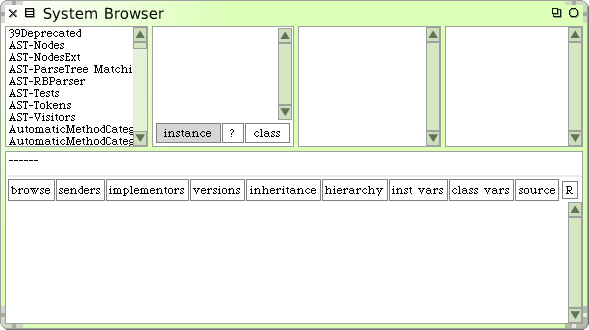
\includegraphics[width=\textwidth]{SystemBrowser0} }
	 {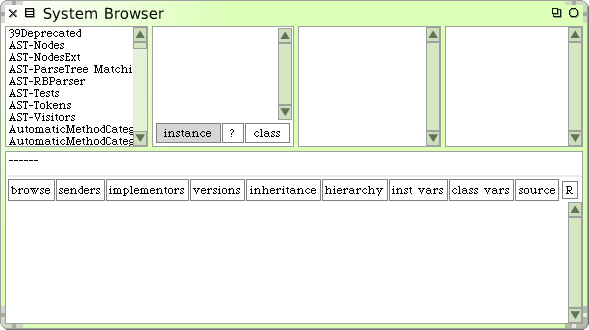
\includegraphics[scale=.7]{SystemBrowser0} }
   \caption{The Browser}
   \label{fig:SystemBrowser0}
\end{figure}

The four small panes at the top of the browser represent a hierarchic view of the methods in the system, much in the same way as the \ind{NeXTstep} \textit{File Viewer} and the Mac OS X \textit{Finder} in column mode provide a view of the files on the disk.
The leftmost pane lists \emph{packages} of classes; select one (say \scat{Kernel}) and the pane immediately to the right will then show all of the classes in that package.
% \on{I adopted the spelling of NeXTstep recommended by wikipedia}

\begin{figure}[htbp]
   \centering
   \ifluluelse
	   {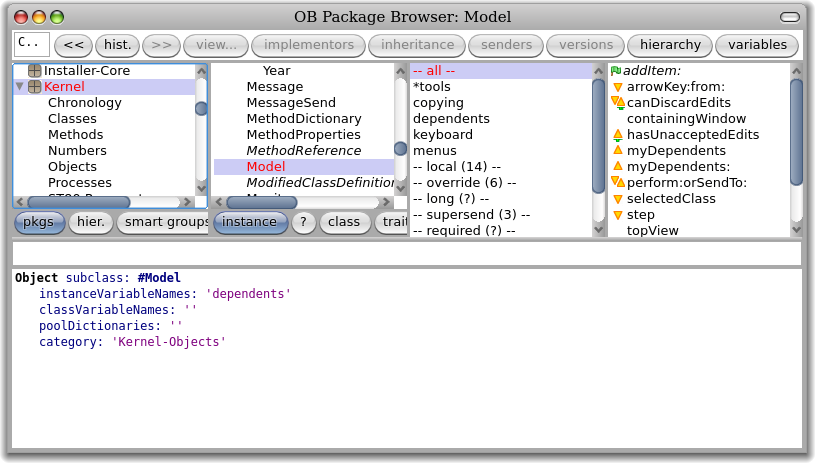
\includegraphics[width=\textwidth]{SystemBrowser1} }
	   {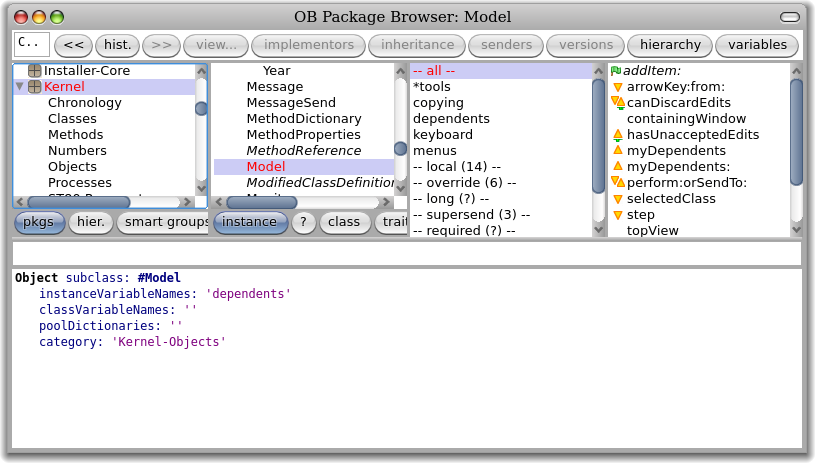
\includegraphics[scale=.7]{SystemBrowser1} }
   \caption{Browser with the class \ct{Model} selected
   \label{fig:SystemBrowserModel}}
\end{figure}

Similarly, if you select one of the classes in the second pane, say, \menu{Model} (see  \figref{SystemBrowserModel}), the third pane will show all of the \emph{protocols} defined for that class, as well as a virtual protocol \prot{-{}-all-{}-}, which is selected by default. 
Protocols are a way of categorizing methods; they make it easier to find and think about the behaviour of a class by breaking it up into smaller, conceptually coherent pieces.  
The fourth pane shows the names of all of the methods defined in the selected protocol.
If you then select a method name, the source code of the corresponding method appears in the large pane at the bottom of the browser, where you can view it, edit it, and save the edited version.
If you select class \menu{Model},  protocol \protind{dependents} and the method \menu{myDependents}, the browser should look like \figref{SystemBrowserMyDependents}.
\protindex{all}
\cmindex{Model}{myDependents}

\begin{figure}[htbp]
   \centering
   \ifluluelse
	   {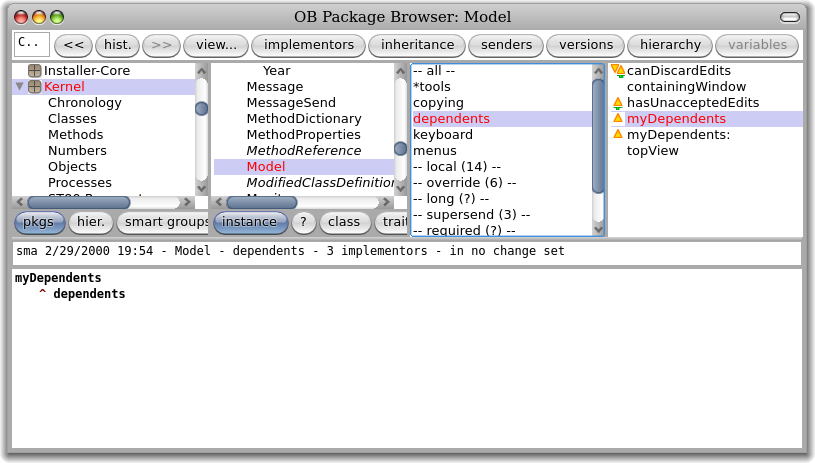
\includegraphics[width=\textwidth]{SystemBrowserMyDependents}}
	   {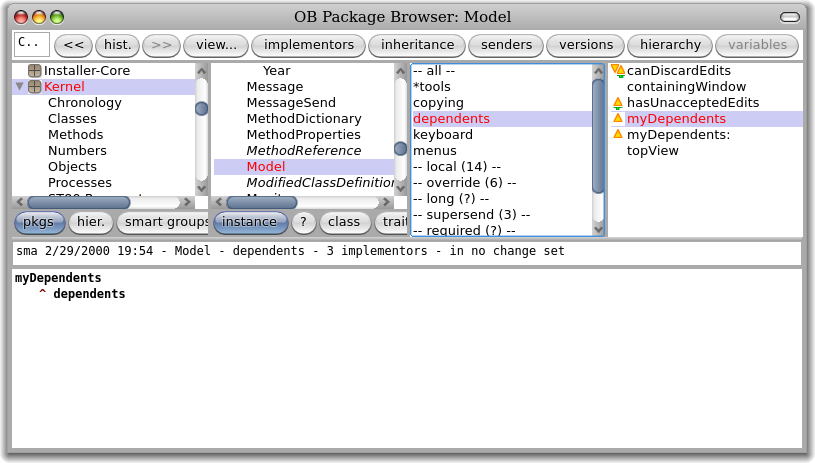
\includegraphics[scale=.7]{SystemBrowserMyDependents}}
   \caption{Browser showing the \ct{myDependents} method in class \ct{Model}
   \label{fig:SystemBrowserMyDependents}}
\end{figure}

Unlike directories in the Mac OS X \emph{Finder}, the four top panes of the browser are not quite equal.  
Whereas classes and methods are part of the Smalltalk language, packages and protocols are not: they are a convenience introduced by the browser to limit the amount of information that needs to be shown in each pane.  For example, if there were no protocols, the browser would have to show a list of all of the methods in the selected class; for many classes this list would be too large to navigate conveniently.  
\index{Mac OS X Finder}

Because of this, the way that you create a new package or a new protocol is different from the way that you create a new class or a new method.  To create a new package, \actclick in the package pane and select \menu{new package}; to create a new protocol, \actclick in the protocol pane and select \menu{new protocol}.
Enter the name of the new thing in the dialog, and you are done: there is nothing more to a category or a protocol than its name and its contents.
\index{category!creating}

\begin{figure}[htbp]
   \centering
   \ifluluelse
	   {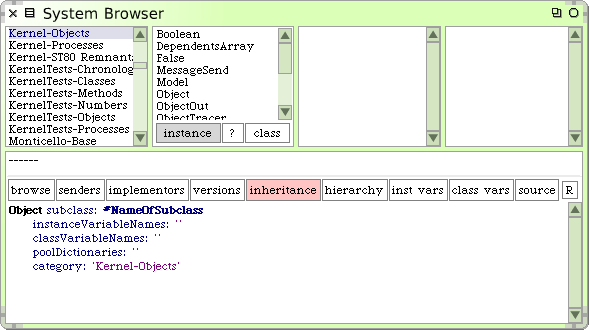
\includegraphics[width=\textwidth]{SystemBrowserClassCreation}}
	   {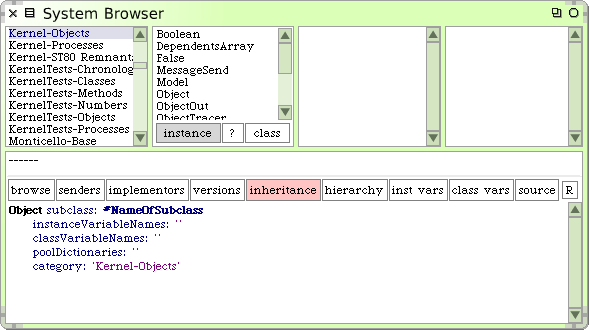
\includegraphics[scale=.7]{SystemBrowserClassCreation}}
   \caption{Browser showing the class-creation template
   \label{fig:SystemBrowserClassCreation}}
\end{figure}

In contrast, to create a new class or a new method, you will actually
have to write some Smalltalk code.  If you deselect the currently
selected category (most left pane) and the reselect it again, the main
browser pane will display a class creation template
(\figref{SystemBrowserClassCreation}).  You create a new class by
editing this template: replace \ct{Object} by the name of the existing
class of which you wish to create a subclass, replace
\ct{NameOfSubclass} by the name that you would like to give to your
new subclass, and fill in the instance variable names if you know
them.  The category for the new class is by default the currently
selected category, but you can change this too if you like.  If you
already have the browser focussed on the class that you wish to
subclass, you can get the same template with slightly different
initialization by \actclick{ing} in the class pane, and
selecting \menu{more \ldots \go subclass template}.  You can also just
edit the definition of an existing class, changing the class name to
something new.  In all cases, when you accept the new definition, the
new class (the one whose name follows the \ct{#}) is created (as is
the corresponding metaclass).  Creating a class also creates a global
variable that references the class, which is why you can refer to all
of the existing classes by using their names.  \index{class!creation}
\index{browser!defining a class}

Can you see why the name of the new class has to appear as a \clsind{Symbol} (\ie prefixed with \ct{#}) in the class creation template, but after the class is created, code can refer to the class by using the name as an identifier (\ie without the \ct{#})?

The process of creating a new method is similar.  First select the class in which you want the method to live, and then select a protocol.  The browser will display a method-creation template, as shown in \figref{SystemBrowserMethodTemplate}, which you can fill-in or edit.
\index{method!creation}
\index{browser!defining a method}

\begin{figure}[htbp]
   \centering
   \ifluluelse
	   {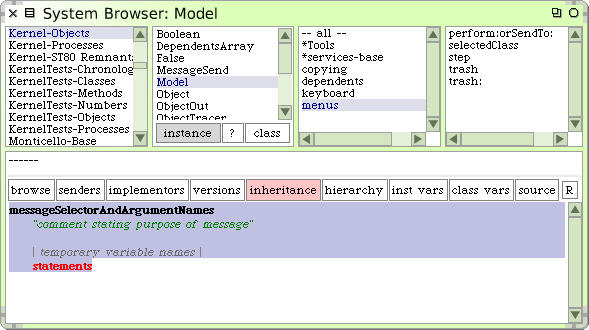
\includegraphics [width=\textwidth]{SystemBrowserMethodTemplate}}
	   {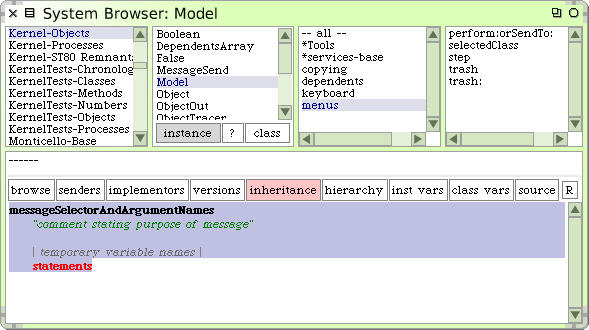
\includegraphics[scale=.7]{SystemBrowserMethodTemplate}}
   \caption{Browser showing the method-creation template
   \label{fig:SystemBrowserMethodTemplate}}
\end{figure}

%---------------------------------------------------------
\subsection{The button bar}
\label{sec:ButtonBar}

The browser provides several tools for exploring and analysing code. Those tools are most simply accessed from the horizontal \subind{browser}{button bar} in the middle of the browser window.  The buttons are labeled \button{browse}, \button{senders}, \button{implementors}\ldots{}\ %
\figref{SystemBrowserMethodTemplate} shows the complete set.

\subsubsection{Browsing code}
\label{sec:browsing}

The \button{browse} button opens a new browser on the class or method that is currently selected. It's often useful to have multiple browsers open at the same time.
When you are writing code you will almost certainly need at least two: one for the method that you are typing, and another to browse around the system to see what to type.
You can also open a browser on a class named by any selected text using the \short{b} \ind{keyboard shortcut}. 
\index{browser!browse button}
\index{keyboard shortcut!browse it}

\dothis{Try this: in a workspace window, type the name of a class (for instance \ct{ScaleMorph}), select it, and then press \short{b}. This trick is often useful; it works in any text window.}

\subsubsection{Senders and implementors of a message}
\label{sec:sendersImplementors}

\index{browser!senders button}
The \button{senders} button will give you a list of all methods that may use the selected method. With the browser open on \ct{ScaleMorph}, click on the \mthind{ScaleMorph}{checkExtent:} method in the method pane near the top right corner of the browser; the body of \ct{checkExtent:} displays in the bottom part of the browser. If you now press the \button{senders} button, a menu will appear with \ct{checkExtent:} as the topmost item, and below it, all the messages that \ct{checkExtent:} sends (see \figref{SendersOfCheckEvent}).  Selecting an item in this menu will open a browser with the list of all methods in the image that send the selected message. 

\begin{figure}[htbp]
	\begin{center}
   \ifluluelse
		{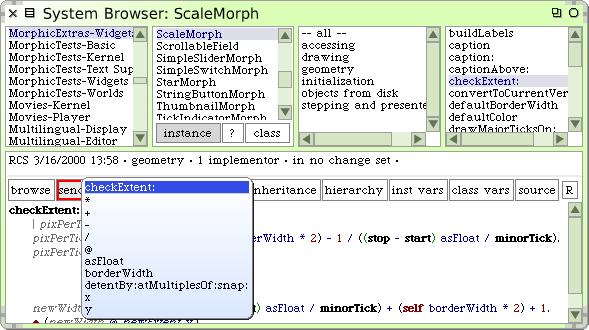
\includegraphics[width=\textwidth]{SendersOfCheckEvent}}
		{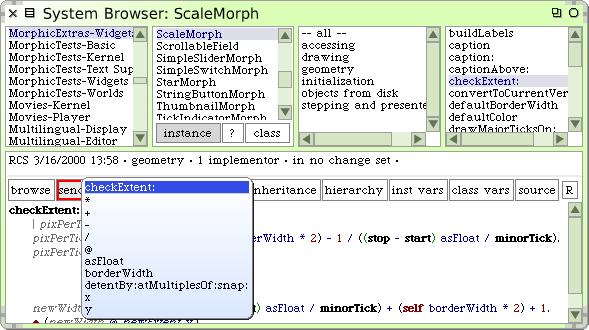
\includegraphics[scale=0.7]{SendersOfCheckEvent}}
	\end{center}
	\caption{A Class Browser opened on the \lct{ScaleMorph} class. Note the horizontal bar of buttons at the center of the browser; here we are using the \lct{senders} button.}
	\label{fig:SendersOfCheckEvent}
\end{figure}

\index{browser!implementors button}
The \button{implementors} button works in a similar way, but instead of listing the senders of a message, it lists all of the classes that implement a method with the same selector. To see this, select \lct{drawOn:} in the message pane and then bring up the ``implementors of drawOn:'' browser, either using the \button{implementors} button, or \actclick{ing} in the method pane, or just by typing \short{m} (for {i\textbf{m}ple\textbf{m}entors}) in the method pane with \menu{drawOn:} selected.  You should get a method list window showing a scrolling list of 96 classes that implement a \ct{drawOn:} method.
It shouldn't be all that surprising that so many classes implement this method: \ct{drawOn:} is the message that is understood by every object that is capable of drawing itself on the screen.  While viewing any one of these methods, try browsing the senders of the \ct{drawOn:} message:  we found 63 methods that send this message.  You can also bring up an implementors browser at any time by selecting a message (including the arguments if it is a keyword message) and typing \short{m}.

%The \menu{senders} button lists \emph{all} the methods that send the chosen message: not all of these message sends will necessarily be able to cause the execution of any particular method with the same selector.
%Indeed, much of the power of object-oriented programming comes from the fact that every message send is potentially \emph{polymorphic}, that is, it can work equally well on objects of any class.  Sometimes it is easy to figure out which method will be executed as result of a particular message send, and sometimes it is impossible; the senders and implementors tools don't try.
% APB: commented-out because the same thought is expressed below.

If you look at the send of \ct{drawOn:} in \ct{AtomMorph>>>drawOn:}, you will see that it is a super \subind{super}{send}.  So we know that the method that will be executed will be in \ct{AtomMorph}'s superclass.  What class is that?  Click the \button{hierarchy} button and you will see that it is \ct{EllipseMorph}. 
\index{browser!hierarchy button}

\begin{figure}[htbp]
	\begin{center}
   \ifluluelse
		{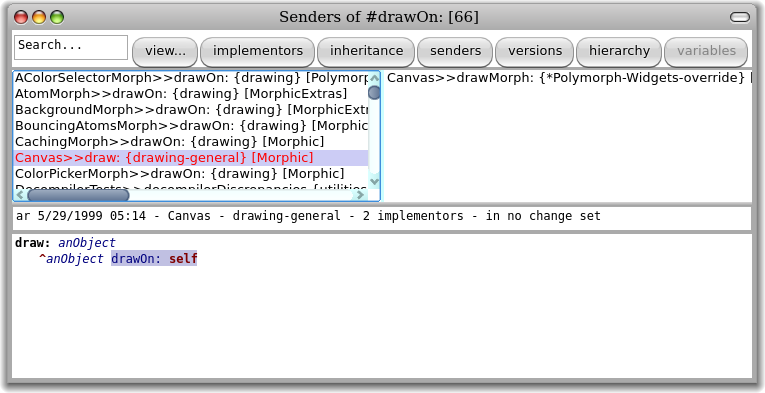
\includegraphics[width=\textwidth]{CanvasDraw}}
		{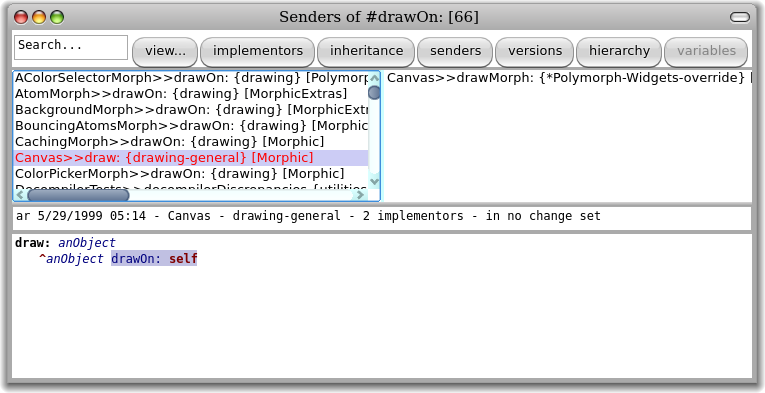
\includegraphics[scale=0.7]{CanvasDraw}}
	\end{center}
	\caption{The Senders Browser showing that the \ct{Canvas>>>draw} method sends the \ct{drawOn:} message to its argument.	\label{fig:CanvasDraw}}
\end{figure}

Now look at the fifth sender in the list, \ct{Canvas>>>draw}, shown in \figref{CanvasDraw}.
You can see that this method sends \ct{drawOn:} to whatever object is passed to it as an argument, which could potentially be an instance of any class at all.  
Dataflow analysis can help figure out the class of the receiver of some messages, but in general, there is no simple way for the browser to know which message-sends might cause which methods to be executed.
For this reason,  the ``senders'' browser shows exactly what its name suggests: all of the senders of the message with the chosen selector.  
The \button{senders} button is nevertheless extremely useful when you need to understand how you can \emph{use} a method: it lets you navigate quickly through example uses.  
Since all of the methods with the same selector ought to be used in the same way, all of the uses of a given message ought to be similar.
\index{browser!senders button}

\subsubsection{Versions of a method}
\label{sec:versions}

When you save a new \subind{method}{version} of a method, the old one is not lost.  \pharo keeps all of the old versions, and allows you to compare different versions and to go back (``revert'') to an old version.
\begin{figure}[btp]
   \centering
   \ifluluelse
	   {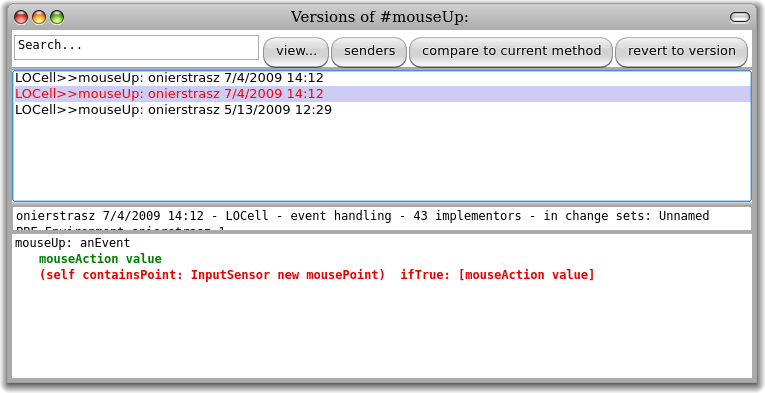
\includegraphics[width=\textwidth]{VersionsOfMouseUp} }
	   {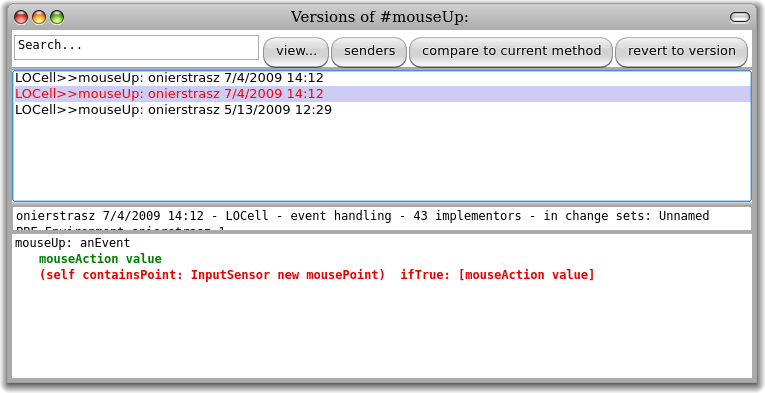
\includegraphics[scale=0.7]{VersionsOfMouseUp} }
   \caption{The \ind{versions browser} showing several versions of the \ct{LOCell>>>mouseUp:} method}
   \label{fig:mouseUpVersions}
\end{figure}
The \button{versions} button gives access to the successive modifications made to the selected method.
In \figref{mouseUpVersions} we can see the versions of the \ct{mouseUp:} method that one of the authors created while writing the Lights Out game described in \charef{firstApp}.

\index{browser!versions button}
The top pane displays one line for each version of the method, listing the initials of the programmer who wrote it, the date and time at which it was saved, the names of the class and the method, and the protocol in which it was defined.  The current (active) version is at the top of the list;  whichever version is selected is displayed in the bottom pane.  If the \menu{diffs} checkbox is selected, as it is in \figref{mouseUpVersions}, the display also shows the differences between the selected version and the one immediately older.  Buttons are also provided for displaying the differences between the selected method and the current version, and for reverting to the selected version.   The \menu{prettyDiffs} checkbox is useful if there have been changes to layout: it pretty-prints both versions before differencing, so that the differences that are displayed exclude formatting changes. 

The existence of the \ind{versions browser} means that you never have to worry about preserving code that you think might no longer be needed: just delete it.  If you find that you \emph{do} need it, you can always revert to the old version, or copy the needed code fragment out of the old version and paste it into a another method.
Get into the habit of using versions;  ``commenting out'' code that is no longer needed is a bad practice because it makes the current code harder to read.
Smalltalkers rate code readability extremely highly.

\hint{What if you delete a method entirely, and then decide that you want it back?  You can find the deletion in a change set, where you can ask to see versions by \actclick{ing}.
The change set browser is described in \secref{env:changeSet}}

\subsubsection{Method overridings}
\label{sec:overriding}

The \button{inheritance} button opens a specialized browser that displays all the methods overridden by the displayed method. 
To see how it works, display the \cmind{ScaleMorph}{defaultColor} method and click \button{inheritance}. This method definition overrides \mbox{\cmind{RectangleMorph}{defaultColor},} which itself overrides \cmind{Morph}{defaultColor}, as shown in \figref{inheritanceOverriding}. The colour of the \button{inheritance} button depends on how the \subind{method}{overriding} occurs.  The colours are explained in a help balloon:
\index{browser!inheritance button}

%\newcommand{\colourTag}[1]{\item[{\mdseries \itshape #1}]}

%\begin{description}[noitemsep, leftmargin=*, labelindent=6em, labelwidth=4em, labelsep=*]
%	\colourTag{pink:} the displayed method overrides another method but doesn't use it;
%	\colourTag{green:} the displayed method overrides another method and uses it via \super;
%	\colourTag{gold:} the displayed method is itself overridden in a subclass;
%	\colourTag{salmon:} the displayed method overrides another method, and it itself overridden;
%	\colourTag{violet:} the displayed method overrides, is overridden, and makes a \ct{super}-send.
%\end{description}

\begin{tabular}{lp{9cm}}
	\emph{pink:} & the displayed method overrides another method but doesn't use it;\\
	\emph{green:} & the displayed method overrides another method and uses it via \super;\\
	\emph{gold:} & the displayed method is itself overridden in a subclass;\\
	\emph{salmon:} & the displayed method overrides another method, and it itself overridden;\\
	\emph{violet:} & the displayed method overrides, is overridden, and makes a \ct!super!-send.
\end{tabular}

\begin{figure}[tbp]
	\begin{center}
   \ifluluelse
		{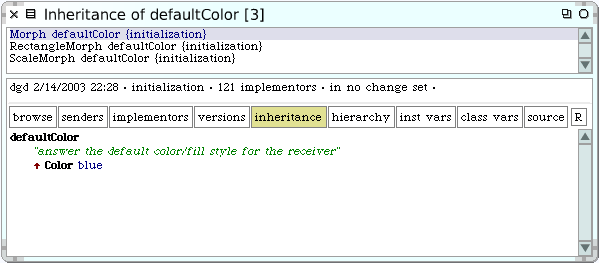
\includegraphics[width=\textwidth]{inheritanceOverriding}}
		{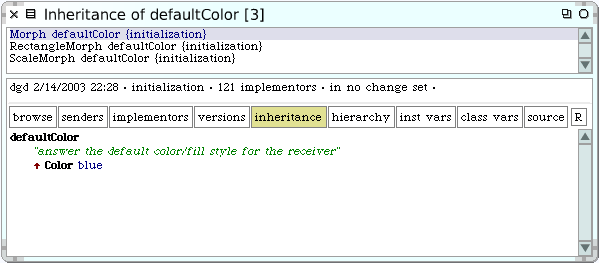
\includegraphics[scale=0.7]{inheritanceOverriding}}
	\end{center}
	\caption{\ct{ScaleMorph>>>defaultColor} and the methods that it overrides, in inheritance order. 
	The \lct{inheritance} button is gold because the displayed method is overridden in a subclass}
	\label{fig:inheritanceOverriding}
\end{figure}

\hyphenation{Omni-Brow-ser}
Note that there are currently two versions of the inheritance browser.  If you are using the version of the browser based on the \ind{OmniBrowser} framework, the \button{inheritance} button does not change colour, and the inheritance browser looks different.  It also displays more information: it shows not only the methods on the inheritance chain, but also their siblings.  This version of the \ind{inheritance browser} is shown in \figref{OBinheritanceBrowser}.

\begin{figure}[btp]
	\begin{center}
   \ifluluelse
		{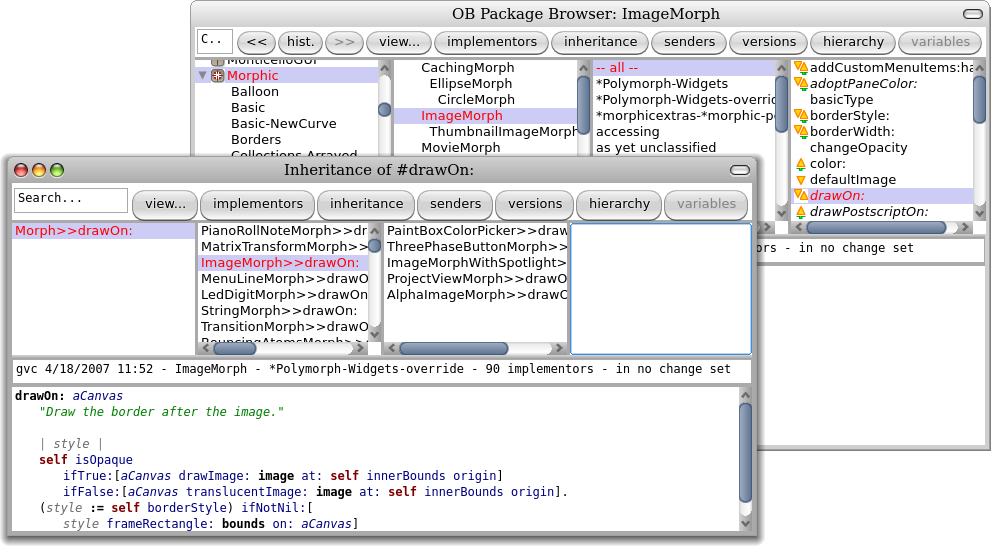
\includegraphics[width=\textwidth]{OBInheritanceOverriding}}
		{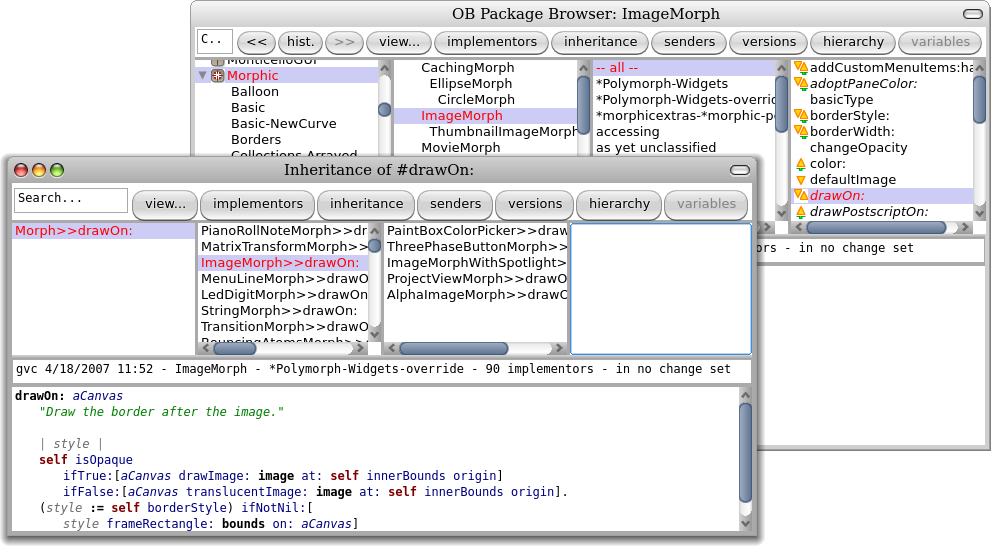
\includegraphics[scale=0.7]{OBInheritanceOverriding}}
	\end{center}
	\caption{\ct{ScaleMorph>>>defaultColor} and the methods that it overrides, as shown by the new OmniBrowser based inheritance browser.   The siblings of the selected methods are shown in the scrolling lists.}
	\label{fig:OBinheritanceBrowser}
\end{figure}


\subsubsection{The Hierarchy Browser}
\label{sec:hierarchy}

The \button{hierarchy} button opens a \ind{hierarchy browser} on the current class; this
browser can also be opened by using the \menu{browse hierarchy} menu item in the class pane.
The hierarchy browser is similar to the browser, but instead of displaying the categories and the classes in each category, it shows a single list of classes, indented to represent inheritance.
The category of the selected class is displayed in the small annotation pane at the top of the browser.
The hierarchy browser is designed to make it easy to navigate through the inheritance hierarchy, but does not show all of the classes in the system: only the superclasses and subclasses of the initial class are shown.
In \figref{hierarchyBrowser}, the hierarchy browser reveals that the direct superclass of \clsind{ScaleMorph} is \clsind{RectangleMorph}.
\index{browser!hierarchy button}

\begin{figure}[btp]
	\begin{center}
	\ifluluelse
		{\includegraphics[width=\textwidth]{hierarchyBrowser}}
		{\includegraphics[scale=0.7]{hierarchyBrowser}}
	\end{center}
	\caption{A hierarchy browser open on \ct{ScaleMorph}.}
	\label{fig:hierarchyBrowser}
\end{figure}

\subsubsection{Finding variable references}
\label{sec:variables}

\index{browser!inst vars button}
\index{browser!class vars button}
The \button{inst vars} and \button{class vars} buttons help you find where an instance variable or a class variable is used; the same information is accessible by \actclick{ing} in the class pane and selecting\menu{inst var refs} and \menu{class var refs}.
The menu also includes \menu{inst var defs}, which shows the subset of the instance variable references that assign to the variable. 
Once you click on the button or select the menu item, you will be presented with a dialog that invites you to choose a variable from all of the variables defined in the current class, and all of the variables that it inherits.  The list is in inheritance order; it can often be useful to bring up this list just to remind yourself of the name of an instance variable.  If you click outside the list, it will go away and no variable browser will be created.

Also available by \actclick{ing} the class pane is \menu{class vars}, which opens an inspector showing the class variables of the current class \emph{and their values}, and \menu{class refs (N)} which displays a list of all of the methods that directly reference the current class.

\subsubsection{Source}
\label{sec:sources}

\index{browser!source button}
The \button{source} button brings up the ``what to show'' menu, which allows you to choose what the browser shows in the source pane.  Options include the \menu{source} code, \menu{prettyPrint}ed source code, \menu{byteCodes} and source code \menu{decompile}d from the byte codes.  The label on the button changes if you select one of the other modes.  There are other options too; if you let the mouse linger over the names, a help balloon will appear.  Try some of them.
\index{method!pretty-print}
\index{method!decompile}
\index{method!byte code}

Note that selecting \menu{prettyPrint} in the ``what to show'' menu is \emph{not} the same as prettyPrinting a method before you save it.  
The menu controls only what the browser displays, and has no effect on the code stored in the system.  
You can verify this  by opening two browsers, and selecting \menu{prettyPrint} in one and \menu{source} in the other.   
In fact, focussing two browsers on the same method and selecting \menu{byteCodes} in one and \menu{decompile} in another is a good way to learn about the \pharo virtual machine's byte-coded instruction set.

\subsubsection{Refactoring}

\index{browser!refactor button}
Did you notice the small \button{R} at the end of the button bar? \fix
Although unobtrusive, this button gives access to one of the most powerful and important features of the Smalltalk environment.  
Clicking on \button{R} gives you access to a hierarchy of menus for refactoring your code.  
The same refactoring engine is also available in several other ways, for example, by \actclick{ing} in the class, method and code panes.
Refactoring was formerly available only in a special browser called the refactoring browser, but it can now be accessed from any browser.

%---------------------------------------------------------
\subsection{The browser menus}

Many additional functions are available by \actclick{ing} in the browser panes..  
Even if the labels on the menu items are the same, their \emph{meaning} is context dependent.  
For example, the category pane, the class pane, the protocol pane and the messages pane all have a \menu{file out} menu item.  However, they do different things: the category pane's \menu{file out} menu files out the whole category, the class pane's \menu{file out} menu files-out the whole class, the protocol pane's \menu{file out} menu files out the whole protocol, and the method pane's \menu{file out} menu files-out just the displayed method.
Although this may seem obvious, it can be a source of confusion for beginners. 
\index{file!filing in}
\index{file!filing out}

Possibly the most useful menu item is \menu{find class\ldots (f)} in the category pane.  Although the categories are useful for the code that we are actively developing, most of us do not know the categorization of the whole system, and it is much faster to type \short{f} followed by the first few characters of the name of a class than to guess which category it might be in.  \menu{recent classes\ldots (r)} can also help you quickly go back to a class that you have browsed recently, even if you have forgotten its name.
\index{class!finding}
\index{class!recent}

In the class pane, there are two menu items \menu{find method} and \menu{find method wildcard\ldots} that can be useful if you want to browse a particular method.  However, unless the list of methods is very long, it is often quicker to browse the \prot{-{}-all-{}-} protocol (which is the default), place the mouse in the method pane, and type the first letter of the name of the method that you are looking for.
This will usually scroll the pane so that the sought-for method name is visible.
\index{method!finding}
\protindex{all}

\dothis{Try both ways of navigating to \cmind{OrderedCollection}{removeAt:}}

There are many other options available in the menus.  It pays to spend a few minutes working with the browser and seeing what is there.   

\dothis{Compare the result of \menu{Browse Protocol}, \menu{Browse Hierarchy},  and \menu{Show Hierarchy} in the class pane menu.}

%---------------------------------------------------------
\subsection{Other browsers}
\label{sec:otherBrowsers}

At the beginning of this section we mentioned another browser: the \emphind{package pane browser}. 
This can be opened from the world menu: \menu{World \go open\ldots \go package pane browser}
It's basically the same as the browser, but it knows about the naming convention for categories.
You will have noticed that the names of categories have two parts.
For example, the \ct{ScaleMorph} class belongs to the \scat{Morphic-Widgets} category.
\label{sec:package-names}
The package browser assumes that the part before the hyphen, \ct{Morphic} is the name of a ``package'', and adds a fifth pane that allows you to browse only those categories in a particular package.
However, if you select no package at all, then all the categories are available, just as with the ordinary four-pane browser.

Unfortunately, the meaning of the term \ind{package} has changed since the package pane browser was developed.  ``Package'' now has a more precise meaning, related to the \emph{Monticello} packaging tool, as we will discuss in the next section.  At present there is no tool that lets you browse packages as defined by \ind{Monticello}, however there is one currently being developed.


\fix

The \pharo community is in the process of developing a whole new family of browsers based on a new, highly customizable framework called the \emphind{OmniBrowser}.  The implementation of the OmniBrowser is worth looking at as a good example of object-oriented design, \ab{and I'ld like to add a chapter on it somewhere, perhaps starting with parts of the excellent document written by Niklaus Haldimann on the classbox browser} but from the outside, most of the OmniBrowser-based tools look very similar to the ones that we have just described.  
The main enhancement that you will notice in the Omni Browser is the addition of \emph{virtual protocols}.
\lr{"Virtual Protocols" are a non-default extension to OB (p. 140)}
In addition to the traditional programmer-defined protocols, each class has a number of virtual protocols defined on it by definitional rules.  For example, the \prot{-{}-supersend-{}-} protocol includes all of the methods that send to \super, while the \prot{-{}-required-{}-} protocol lists all of the messages that are sent by the methods in the current class or its superclasses but not defined.
\protindex{supersend}
\protindex{required}

\on{Is this related to abstract methods or not?  It is not clear.}

\ab{You are right, it's not clear.  The definition of abstract method that we have given is a method that has \ct{self subclassResponsibility} as a body.
By this definition, the two things are different.  I happen to think that the definition that we used for required method is better, and should be adopted for abstract method, \ie an abstract method is one that is either required, or has a marker method \ct{self subclassResponsibility} or \ct{self explicitRequirment}.}

\on{So, what should we say? As it stands, without comment it is confusing. Everyone will ask: uh ... is this different from an abstract method?}

%---------------------------------------------------------
\subsection{Browsing programmatically}

The class \glbind{SystemNavigation} provides a number of utility methods that are useful for navigating around the system.
Many of the functions offered by the classic browser are implemented by \ct{SystemNavigation}.
\index{browsing programmatically}

\dothis{
Open a workspace and \menu{do it} the following code to browse the senders of \ct{checkExtent:}:}
\begin{code}{}
SystemNavigation default browseAllCallsOn: #checkExtent: .
\end{code}
To restrict the search for senders to the methods of a specific class:
\begin{code}{}
SystemNavigation default browseAllCallsOn: #drawOn: from: ScaleMorph .
\end{code}
Because the development tools are objects, they are completely accessible from programs and you can develop your own tools or adapt the existing tools to your needs.

The programmatic equivalent to the \button{implementors} button is:
\begin{code}{}
SystemNavigation default browseAllImplementorsOf: #checkExtent: .
\end{code}

To learn more about what is available, explore the class \ct{SystemNavigation} with the browser.
Further navigation examples can be found in the FAQ (\appref{faq}).

\lr{Maybe mention how to change the default browser? SystemBrowser askForDefault (p. 141)}

%---------------------------------------------------------
\subsection{Summary}

As you have seen, there are many ways to navigate around Smalltalk code. 
You may find this confusing at first, in which case you can always fall back to the traditional browser.
However, we usually find that once beginners gain more experience with \pharo, the availability of different browsers becomes one of its most valued features, because they provide many ways to help you to understand and organize your code.
The problem of understanding code is one of the greatest challenges of large-scale software development. 
% section browser (end)

%=========================================================
\section{Monticello}

We gave you a quick overview of \ind{Monticello}, \pharo's packaging tool, in \secref{Monticello}.  
However, Monticello has many more features than were discussed there.  
Because Monticello manages \emph{Packages}, before telling you more about Monticello, it's important that we first explain exactly what a \ind{package} is.

%---------------------------------------------------------
\subsection{Packages: declarative categorization of \pharo code}

The package system is a simple, lightweight way of organizing Smalltalk source code.
It leverages the long-used naming convention mentioned above (\secref{package-names}), but adds to it in an important way.

Let's explain this using an example.
Suppose that you are developing a framework named to facilitate the use of relational databases from \pharo. You have decided to call your framework \ct{PharoLink}, and have created a series of categories to contain all of the classes that you have written, \eg

\vspace{1ex}
\noindent
Category \ct{'PharoLink-Connections'} contains \ct{OracleConnection MySQLConnection PostgresConnection}\\
Category \ct{'PharoLink-Model'} contains \ct{DBTable DBRow DBQuery}

\vspace{1ex}
\noindent
and so on. However, not all of your code will reside in these classes. For example, you may also have a series of methods to convert objects into an SQL-friendly format:

\begin{code}{}
Object>>>asSQL
String>>>asSQL
Date>>>asSQL
\end{code}

\noindent
These methods belong in \damien{don't we say 'belong to'?} the same package as the classes in the 
categories \ct{PharoLink-Connections} and \ct{PharoLink-Model}. 
But clearly the whole of class \ct{Object} does not belong in your package! 
So you need a way of putting certain \emph{methods} in a package, even though the rest of the class is in another package.
\index{package!extension}
\seeindex{extension package}{package, extension}

The way that you do this is by placing those methods in a protocol (of \ct{Object}, \ct{String}, \ct{Date}, and so on) named \prot{*PharoLink} (note the initial asterisk, and the {\fix} lower-case name). The combination of the \scat{PharoLink-...} categories and the \prot{*PharoLink} protocols form a package named \ct{PharoLink}.
To be precise, the rules for what goes in a package are as follows.

A package named \ct{Foo} contains:

\begin{enumerate}		\label{sec:packageRules}
	\item{} all class definitions of classes in the category \scat{Foo}, or in categories with names starting with \scat{Foo-}, and
	\item{} \label{env:extensions} all method definitions in any class in a protocol named \prot{*foo} or whose name starts with \prot{*foo-} (when performing this name comparison, the case of the letters in the names is ignored), and
	\item{} all methods in classes in the category \scat{Foo}, or in a category whose name starts with \scat{Foo-}, \emph{except} for those methods in protocols whose names start with \prot{*}.
	
\end{enumerate}
\noindent
A consequence of these rules is that each class definition and each method belongs to exactly one package. The \emph{except} in the last rule has to be there because those methods must belong to other packages.   The reason for ignoring case in rule \ref{env:extensions} is that, by convention, protocol names are all lower case (and may include spaces), while category names use CamelCase (and don't include spaces).
\index{camelCase}

The class \ct{PackageInfo} implements these rules, and one way to get a feel for them is to experiment with this class.

\dothis{Try this in your image, which should contain the classes \ct{PackageInfo} and \ct{RefactoringBrowser.}}
The Refactoring Browser code uses these package naming conventions, with \lct{Refactoring\-Engine} as the package name. In a workspace, create a model of this package with
\index{refactoring}

\begin{code}{}
refactory := PackageInfo named: 'RefactoringEngine'. 
\end{code}

It is now possible to introspect on this package. 
For example, \ct{refactory classes} will return the long list of classes that make up the Refactoring Engine and the Refactoring Browser.  
\ct{refactory coreMethods}
will return a list of \ct{MethodReference}s for all of the methods in those classes. \ct{refactory extensionMethods} is perhaps one of the most interesting queries: it will return a list of all methods contained in the \ct{RefactoringEngine} package but not contained within a \lct{Refactoring\-Engine} class. This includes, for example, \ct{ClassDescription>>>chooseThisClassInstVarThenDo:} and \ct{SharedPool class>>>keys}.

Packages are a relatively new addition to \pharo, but since the package naming conventions were based on those already in use, it is possible to use \ct{PackageInfo} to analyze older code that has not been explicitly adapted to work with it.

\dothis{Evaluate  \ct{(PackageInfo named: 'Collections') externalSubclasses}; this expression will answer a list of all subclasses of  \ct{Collection} that are \emph{not} in the \ct{Collections} package. }

You can send \ct{fileOut} to an instance of \ct{PackageInfo} to get a change set of the
entire package.  For more sophisticated versioning of packages, we use Monticello.
\index{file!filing out}

%---------------------------------------------------------
\subsection{Basic Monticello}

\ind{Monticello} is named after the mountaintop home of Thomas Jefferson, third president of the United States and author of the Statute of Virginia for Religious Freedom.  The name means ``little mountain'' in Italian, and so it is always pronounced with an Italian ``c'', which sounds like the ``ch'' in chair: Mont-y'-che-llo.


\begin{figure}[btp]
	\begin{center}
	\ifluluelse
		{\includegraphics[width=\textwidth]{freshMonticello}}
		{\includegraphics[scale=0.7]{freshMonticello}}
	\end{center}
	\caption{The Monticello browser.}
	\label{fig:freshMonticello}
\end{figure}

When you open the Monticello browser, you will see two list panes and a row of buttons, as shown in \figref{freshMonticello}.
The left-hand pane lists all of the packages that have been loaded into the image that you are running; the particular version of the package is shown in parentheses after the name.

The right-hand pane lists all of the source-code repositories that Monticello knows about, usually because it has loaded code from them.  If you select a package in the left pane, the right pane is filtered to show only those repositories that contain versions of the selected package.

One of the repositories is a directory named \emph{package-cache}, which is a sub-directory of the directory in which your image is running.  
When you load code from or write code to a remote repository, a copy is also saved in the package cache.  This can be useful if the network is not available and you need to access a package.  Also, if you are given a Monticello (.mcz) file directly, for example as an email attachment, the most convenient way to access it is to place it in the package-cache directory.
\index{package!cache}

To add a new repository to the list, click the \button{+Repository}, and choose the kind of repository from the pop-up menu.  Let's add an HTTP repository.

\dothis{Open Monticello, click on \button{+Repository}, and select \menu{HTTP}.
Edit the dialog to read:}
%\ab{How does one continue the $\backslash$dothis to include the code?}
%\on{Don't.  Just close the \dothis{} and follow with the code.}
\needlines{4}
\begin{code}{}
MCHttpRepository
	location: 'http://squeaksource.com/PharoByExample'
	user: ''
	password: ''
\end{code}

\begin{figure}[btp]
	\begin{center}
	\ifluluelse
		{\includegraphics[scale=0.65]{SqueakSource-SBE}}
		{\includegraphics[scale=0.7]{SqueakSource-SBE}}
	\end{center}
	\caption{A Repository browser.}
	\label{fig:SqueakSource:PBE}
\end{figure}
\noindent
\fix \on{fix image -- PBE not SBE}
Then click on \button{Open} to open a repository browser on this repository.  You should see something like \figref{SqueakSource:PBE}.  On the left is a list of all of the packages in the repository; if you select one, then the pane on the right will show all of the versions of the selected package in this repository. 

If you select one of the versions, you can \button{Browse} it (without loading it into your image), \button{Load} it, or look at the \button{Changes} that will be made to your image by loading the selected version.  You can also make a \button{Copy} of a version of a package, which you can then write to another repository.

As you can see, the names of versions contain the name of the package, the initials of the author of the version, and a version number.  The version name is also the name of the file in the repository.  Never change these names; correct operation of Monticello depends on them!   Monticello version files are just zip archives, and if you are curious you can unpack them with a zip tool, but the best way to look at their contents is using Monticello itself.  

To create a package with Monticello, you have to do two things: write some code, and tell Monticello about it.

\dothis{Create a category called \scat{PBE-Monticello}, and put a couple of classes in it, as shown in \figref{MCnewcategory}.  Also, create a method in an existing class, and put it in the same package as your classes, using the rules from page \pageref{sec:packageRules}\,---\,see \figref{MCnewmethod}.}

\begin{figure}[btp]
	\begin{center}
	\ifluluelse
		{\includegraphics[width=\textwidth]{MCnewcategory}}
		{\includegraphics[scale=0.7]{MCnewcategory}}
	\end{center}
	\caption{Two classes in the ``PBE'' package.}
	\label{fig:MCnewcategory}
\end{figure}

\begin{figure}[btp]
	\begin{center}
	\ifluluelse
		{\includegraphics[width=\textwidth]{MCnewmethod}}
		{\includegraphics[scale=0.7]{MCnewmethod}}
	\end{center}
	\caption{An extension method that will also be in the ``PBE'' package.}
	\label{fig:MCnewmethod}
\end{figure}

To tell Monticello about your package, click on \button{+Package}, and type the name of the package, in this case ``PBE''.  Monticello will add \ct{PBE} to its list of packages; the package entry will be marked with an asterisk to show that the version in the image has not yet been written to any repository.

Initially, the only repository associated with this package will be your package cache, as shown in \figref{MC+SBE}.  That's OK: you can still save the code, which will cause it to be written to the package cache.  
Just click \button{Save} and you will be invited to provide a log message for the version of the package that you are about to save, as shown in \figref{PBE-apb}; when you accept the message, Monticello will save your package.
To indicate this, the asterisk decorating the name in Monticello's package pane will be removed, and the version number added.

If you then make a change to the package\,---\,say by adding a method to one of the classes\,---\,the asterisk will re-appear, showing that you have unsaved changes.  If you open a repository browser on the package cache, you can select the saved version, and use \button{Changes} and the other buttons.  
You can of course save the new version to the repository too; once you \button{Refresh} the repository view, it should look like \figref{package-cache-browser}.
\index{package!cache}

\begin{figure}[tbp]
	\begin{center}
		\includegraphics[width=\textwidth]{MC+SBE}
		% \on{Sorry Andrew, this one is too wide!}
		% \includegraphics[scale=0.7]{MC+PBE}
	\end{center}
	\caption{The as-yet-unsaved PBE package in Monticello.}
	\label{fig:MC+SBE}
\end{figure}

\begin{figure}[tbp]
	\begin{center}
	\ifluluelse
		{\includegraphics[scale=0.65]{SBE-apb}}
		{\includegraphics[scale=0.7]{SBE-apb}}
	\end{center}
	\caption{Providing a log message for a new version of a package.}
	\label{fig:PBE-apb}
\end{figure}

\on{FIX -> PBE-apb}

\begin{figure}[tbp]
	\begin{center}
	\ifluluelse
		{\includegraphics[scale=0.65]{package-cache-browser}}
		{\includegraphics[scale=0.7]{package-cache-browser}}
	\end{center}
	\caption{Two versions of our package are now in the package cache.}
	\label{fig:package-cache-browser}
\end{figure}

To save the new package to a repository other than the package cache, you need to first make sure that Monticello knows about the repository, adding it if necessary.  
Then you can use the \button{Copy} in the package-cache repository browser, and select the repository to which the package should be copied.  
You can also associate the desired repository with the package by \actclick{ing} on the repository and selecting \menu{add to package...}, as shown in \figref{associateRepository}.  
Once the package knows about a repository, you can save a new version by selecting the repository and the package in the Monticello Browser, and clicking \button{Save}.  
Of course, you must have permission to write to a repository.  
The \ct{PharoByExample} repository on \emphind{\sqsrc} is world readable but not world writable, so if you try and save there, you will see an error message.  
However, you can create your own repository on \sqsrc by using the web interface at \url{http://www.squeaksource.com}, and use this to save your work. 
This is especially useful as a mechanism to share your code with friends, or if you use multiple computers.

\begin{figure}[tbp]
	\begin{center}
		\includegraphics[width=\textwidth]{MCaddToPackage}
	\end{center}
	\caption{Adding a repository to the set of repositories associated with a package.}
	\label{fig:associateRepository}
\end{figure}

If you do try and save to a repository where you don't have write permission, a version will nevertheless be written to the package-cache.  
So you can recover by editing the repository information (\actclick in the Monticello Browser) or choosing a different repository, and then using \button{Copy} from the package-cache browser.

%=========================================================
\section{The Inspector and the Explorer}
\label{sec:inspector} % (fold)

One of the things that makes \st so different from many other programming environments is that it is provides you with a window onto a world of live objects, not a world of static code.
Any of those objects can be examined by the programmer, and even changed\,---\,although some care is necessary when changing the basic objects that support the system.  
By all means experiment, but save your image first!

%---------------------------------------------------------
\subsection{The Inspector}

\dothis{As an illustration of what you can do with an \ind{inspector}, type  \ct{TimeStamp now} in a workspace, and then \actclick and choose \menu{inspect it}.} 
(It's not necessary to select the text before using the menu; if no text is selected, the menu operations work on the whole of the current line.
You can also type \short{i} for \menu{\textbf{i}nspect it}.)
\clsindex{TimeStamp}
\index{keyboard shortcut!inspect it}

\begin{figure}[btp]
	\begin{center}
		\includegraphics[scale=0.65]{inspectTimeNow1}
	\end{center}
	\caption{Inspecting \ct{TimeStamp now}}
	\label{fig:inspectTimeNow1}
\end{figure}

A window like that shown in \figref{inspectTimeNow1} will appear.   
This is an inspector, and can be thought of as a window onto the internals of a particular object\,---\,in this case, the particular instance of \mbox{\ct{TimeStamp}} 
% the \mbox is here because without it, the listings macros puts a space between TimeStamp 
% and the following word, and that space happens to come out at the start of a line.
that was created when you evaluated the expression \ct{TimeStamp now}.
The title bar of the window shows the \emph{class} of the object that is being inspected.
If you select \menu{self} at the top of the left pane, the right pane will show the printstring of the object.
If you select \menu{all inst vars} in the left pane, the right pane will show a list of the instance variables in the object, and the printstring for each one.  
The remaining items in the left pane represent the instance variables; this makes it easy to examine them one at a time, and also to change them.

The horizontal pane at the bottom of the inspector is a small workspace window.  It is useful because in this window, the pseudo-variable \ct{self} is bound to the very object that you are inspecting.  
So, if you \menu{inspect it} on
\begin{code}{}
self - TimeStamp today
\end{code}
in the workspace pane, the result will be a \clsind{Duration} object that represents the time interval between midnight today and the instant at which you evaluated  \ct{TimeStamp now} and created the \ct{TimeStamp} object that you are inspecting.
You can also try evaluating \ct{TimeStamp now - self}; this will tell you how long you have spent reading this section of this book!

In addition to \ct{self}, all the instance variables of the object are in scope in the workspace pane, so you can use them in expressions or even assign to them.  For example, if you evaluate \ct{jdn  := jdn - 1} in the workspace pane, you will see that the value of the \ct{jdn} instance variable will indeed change, and the value of \ct{TimeStamp now - self} will increase by one day.

You can change instance variables directly by selecting them, replacing the old value in the right-hand  pane by a \pharo expression, and accepting.  
\pharo will evaluate the expression and assign the result to the instance variable.

\begin{figure}[tbp]
\begin{minipage}{0.48\textwidth}
	\begin{center}
	\ifluluelse
		{\includegraphics[width=\textwidth]{exploreTimeStampNow}}
		{\includegraphics[scale=0.7]{exploreTimeStampNow}}
	\end{center}
	\caption{Exploring \ct{TimeStamp now}}
	\label{fig:exploreTimeStampNow}
\end{minipage}
\hfill
\begin{minipage}{0.48\textwidth}
	\begin{center}
	\ifluluelse
		{\includegraphics[width=\textwidth]{exploreTimeStampNow2}}
		{\includegraphics[scale=0.7]{exploreTimeStampNow2}}
	\end{center}
	\caption{Exploring the instance variables}
	\label{fig:exploreTimeStampNow2}
\end{minipage}
\end{figure}

There are special variants of the inspector for Dictionaries, OrderedCollections, CompiledMethods and a few other classes that make it easier to examine the contents of these special objects.

%---------------------------------------------------------
\subsection{The Object Explorer}

The \emph{object explorer} is conceptually similar to the inspector, but presents its information in a different way.
To see the difference, we'll \emph{explore} the same object that we were just inspecting.

\dothis{Select \menu{self} in the inspector's left-hand pane, then \actclick and choose \menu{explore (I)}.}
The \ind{explorer} window looks like \figref{exploreTimeStampNow}.
If you click on the small triangle next to \ct{root}, the view will change to \figref{exploreTimeStampNow2}, which shows the instance variables of object that you are exploring.
Click on the triangle next to \ct{offset}, and you will see \emph{its} instance variables.  
The explorer is really useful when you need to explore a complex hierarchic structure\,---\,hence the name.
\index{keyboard shortcut!explore it}

The workspace pane of the object explorer works slightly differently to that of the inspector.
\ct{self} is not bound to the root object, but rather to the object that is currently selected; the instance variables of the selected object are also in scope.
% ON: Fixed. Inadvertently left off the "l" in \lr
\lr{Maybe explain what "self" refers too in the inspector (always the object) and explorer (the selected item) (p. 154)}

To see the value of the explorer, let's use it to explore a deeply-nested structure of objects.

\dothis{Open a browser, and blue-click twice on the method pane to bring-up the Morphic halo on the \ct{PluggableListMorph} that is used to represent the list of messages. 
Click on the \emph{debug} handle \debugHandle{} and select \menu{explore morph}
from the menu that appears.  This will open an Explorer on the \clsind{PluggableListMorph} object that represents the method list on the screen.  
Open the root object (by clicking in its triangle), open its \ct{submorphs}, and continue exploring the structure of the objects that underlie this Morph, as shown in \figref{explorePluggableListMorph}.}

\begin{figure}[tbp]
	\begin{center}
		\includegraphics[scale=0.7]{explorePluggableListMorph}
	\end{center}
	\caption{Exploring a \ct{PluggableListMorph}}
	\label{fig:explorePluggableListMorph}
\end{figure}

%=========================================================
\section{The Debugger}
\label{sec:debugger} % (fold)

The \ind{debugger} is arguably the most powerful tool in the \pharo tool suite.  It is used not just for debugging, but also for writing new code.
To demonstrate the debugger, let's start by writing a bug!

\dothis{Using the browser, add the following method to the class \ct{String}:}

\needspace{10ex}
\begin{method}[buggy]{A buggy method}
suffix
	"assumes that I'm a file name, and answers my suffix, the part after the last dot"
	| dot dotPosition |
	dot := FileDirectory dot.
	dotPosition := (self size to: 1 by: -1) detect: [ :i | (self at: i) = dot ].
	^ self copyFrom: dotPosition to: self size 
\end{method}

Of course, we are sure that such a trivial method will work, so instead of writing an SUnit test, we just type
\ct{'readme.txt' suffix} in a workspace and \menu{print it (p)}.
What a surprise!  Instead of getting the expected answer \ct{'txt'}, a \clsind{PreDebugWindow} pops up, as shown in \figref{PreDebugWindow}.

\begin{figure}[btp]
	\begin{center}
	\ifluluelse
		{\includegraphics[scale=0.65]{PreDebugWindow}}
		{\includegraphics[scale=0.7]{PreDebugWindow}}
	\end{center}
	\caption{A \ct{PreDebugWindow} notifies us of a bug.}
	\label{fig:PreDebugWindow}
\end{figure}

The \ct{PreDebugWindow} has a title-bar that tells us what error occurred, and shows us a \emphind{stack trace} of the messages that led up to the error. 
Starting from the bottom of the trace, \ct{UndefinedObject>>>DoIt} represents the code that was compiled and run when we selected \ct{'readme.txt' suffix} in the workspace and asked \pharo to \menu{print it}.
This code, of course, sent the message \ct{suffix} to a \clsind{ByteString} object (\ct{'readme.txt'}). 
This caused the inherited \ct{suffix} method in class \ct{String} to execute; all this information is encoded in the next line of the stack trace, \ct{ByteString(String)>>>suffix}.  
Working up the stack, we can see that \ct{suffix} sent \ct{detect:}\ldots and eventually \ct{detect:ifNone} sent \ct{errorNotFound}.
\clsindex{UndefinedObject}

\begin{figure}[btp]
	\begin{center}
	\ifluluelse
		{\includegraphics[width=\textwidth]{debuggerDetectIfNone}}
		{\includegraphics[scale=0.7]{debuggerDetectIfNone}}
	\end{center}
	\caption{The debugger.}
	\label{fig:debuggerDetectIfNone}
\end{figure}

To find out \emph{why} the dot was not found, we need the debugger itself, so click on \button{Debug}.

\dothis{You can also open the debugger by clicking on any of the lines on the stack trace.  If you do this, the debugger will open already focussed on the corresponding method.}

The debugger is shown in \figref{debuggerDetectIfNone}; it looks intimidating at first, but it is quite easy to use.
The title-bar and the top pane are very similar to those that we saw in the \lct{PreDebugWindow}.  
However, the debugger combines the stack trace with a method browser, so when you select a line in the stack trace, the corresponding method is shown in the pane below.
It's important to realize that the execution that caused the error is still in your image, but in a suspended state.  
Each line of the stack trace represents a frame on the execution stack that contains all of the information necessary to continue the execution.  This includes all of the objects involved in the computation, with their instance variables, and all of the temporary variables of the executing methods.

In \figref{debuggerDetectIfNone} we have selected the \ct{detect:ifNone:} method in the top pane.
The method body is displayed in the center pane; the blue highlight around the message \ct{value} shows that the current method has sent the message \ct{value} and is waiting for an answer.

The four panes at the bottom of the debugger are really two mini-inspectors (without workspace panes).
The inspector on the left shows the current object, that is, the object named \self in the center pane.
As you select different stack frames, the identity of \self may change, and so will the contents of the 
\self{}-inspector.
If you click on \self in the bottom-left pane, you will see that \self is the interval \ct{(10 to: 1 by -1)}, which is what we expect.
The workspace panes are not needed in the debugger's mini-inspectors because all of the variables are also in scope in the method pane; you should feel free to type or select expressions in this pane and evaluate them.  
You can always \menu{cancel (l)} your changes using the menu or \short{\textit{l}}. 
% apb: that lower-case-L is in italics so that it doesn't look like a 1 or a |
\index{keyboard shortcut!cancel}

The inspector on the right shows the temporary variables of the current context.
In \figref{debuggerDetectIfNone},
\ct{value} was sent to the parameter \ct{exceptionBlock}.

\dothis{To see the current value of this parameter, click on \ct{exceptionBlock} in the context inspector.
This will tell you that \ct{exceptionBlock} is \ct{[self errorNotFound: ...]}.
So, it is not surprising that we see the corresponding error message.}

Incidentally, if you want to open a full inspector or explorer on one of the variables shown in the mini-inspectors, just double-click on the name of the variable, or select the name of the variable and \actclick to choose \menu{inspect (i)} or \menu{explore (I)}.
This can be useful if you want to watch how a variable changes while you execute other code. 
\index{keyboard shortcut!inspect it}
\index{keyboard shortcut!explore it}

Looking back at the method window, we see that we expected the penultimate line of the method to find \ct{dot} in the string \ct{'readme.txt'}, and that execution should never have reached the final line.
\pharo does not let us run an execution backwards, but it does let us start a method again, which works very well in code such as this that does not mutate objects, but instead creates new ones.  

\dothis{Click \button{Restart}, and you will see that the locus of execution returns to the first statement of the current method.  
The blue highlight shows that the next message to be sent will be {\ct{do:}} (see \figref{RestartDetectIfNone}).}

\begin{figure}[btp]
	\begin{center}
	\ifluluelse
		{\includegraphics[width=\textwidth]{RestartDetectIfNone}}
		{\includegraphics[scale=0.7]{RestartDetectIfNone}}
	\end{center}
	\caption{The debugger after restarting the \ct{detect: ifNone:} method}
	\label{fig:RestartDetectIfNone}
\end{figure}

The \button{Into} and \button{Over} buttons give us two different ways to step through the execution.  If you click \button{Over}, \pharo executes the current message-send (in this case the \ct{do:}) in one step, unless there is an error.  
So \button{Over} will take us to the next message-send in the current method, which is \ct{value}: this is exactly where we started, and not much help. 
What we need to do is to find out why the \ct{do:} is not finding the character that we are looking for.

\dothis{Click \button{Over}, and then click \button{Restart} to get back to the situation shown in \figref{RestartDetectIfNone}.}

\dothis{Click \button{Into}; \pharo will go into the method corresponding to the highlighted message-send, in this case, \ct{Collection>>>do:}.}

However, it turns out that this is not much help either: we can be fairly confident that \ct{Collection>>>do:} is not broken.  The bug is much more likely to be in \emph{what} we asked \pharo to do.
\button{Through} is the appropriate button to use in this case: we want to ignore the details of the \ct{do:} itself and focus on the execution of the argument block. 

\dothis{Click on \button{Through} a few times.  Select \ct{each} in the context window as you do so.
You should see \ct{each} count down from \ct{10} as the \ct{do:} method executes.}

When \ct{each} is \ct{7} we expect the \ct{ifTrue:} block to be executed, but it isn't.
To see what is going wrong, go \button{Into} the execution of \ct{value:} as illustrated in \figref{steppingIntoValue}.

\begin{figure}[btp]
	\begin{center}
	\ifluluelse
		{\includegraphics[width=\textwidth]{steppingIntoValue}}
		{\includegraphics[scale=0.7]{steppingIntoValue}}
	\end{center}
	\caption{The debugger after stepping \lct{Through} the \ct{do:} method several times}
	\label{fig:steppingIntoValue}
\end{figure}

After clicking \button{Into}, we find ourselves in the position shown in \figref{dotIsAString}.
It looks at first that we have gone \emph{back} to the \ct{suffix} method, but this is because we are now executing the block that \ct{suffix} provided as argument to \ct{detect:}.  
If you select \ct{i} in the context inspector, you can see its current value, which should be \ct{7} if you have been following along.  
You can then select the corresponding element of \self from the \self{}-inspector.
In  \figref{dotIsAString} you can see that element \ct{7} of the string is character 46, which is indeed a dot.
If you select \ct{dot} in the context inspector, you will see that its value is \ct{'.'}.
And now you see why they are not equal: the seventh character of \ct{'readme.txt'} is of course a \ct{Character}, while \ct{dot} is a \ct{String}.

\begin{figure}[btp]
	\begin{center}
	\ifluluelse
		{\includegraphics[width=\textwidth]{dotIsAString}}
		{\includegraphics[scale=0.7]{dotIsAString}}
	\end{center}
	\caption{The debugger showing why \ct{'readme.txt' at: 7} is not equal to \ct{dot}}
	\label{fig:dotIsAString}
\end{figure}

Now that we see the bug, the fix is obvious: we have to convert \ct{dot} to a character before starting to search for it.  

\begin{figure}[btp]
	\begin{center}
	\ifluluelse
		{\includegraphics[width=\textwidth]{revertDialog}}
		{\includegraphics[scale=0.7]{revertDialog}}
	\end{center}
	\caption{Changing the \ct{suffix} method in the debugger: asking for confirmation of the exit from an inner block}
	\label{fig:revertDialog}
\end{figure}

\dothis{Change the code right in the debugger so that the assignment reads \ct{dot := FileDirectory dot first} and \menu{accept} the change.}
\on{NB: String>>asCharacter is now deprecated! use first instead}
Because we are executing code inside a block that is inside a \lct{detect:}, several stack frames will have to be abandoned in order to make this change.  \pharo asks us if this is what we want (see \figref{revertDialog}), and, assuming that we click \menu{yes}, will save (and compile) the new method.

\dothis{Click \button{Restart} and then \button{Proceed}; the debugger window will vanish, and the evaluation of the expression \ct{'readme.txt' suffix} will complete, and print the answer \ct{'.txt'}}

Is the answer correct?  Unfortunately, we can't say for sure.  Should the suffix be \ct{.txt} or \ct{txt}?
The method comment in \ct{suffix} is not very precise.  
The way to avoid this sort of problem is to write an \ind{SUnit} test that defines the answer.

\begin{method}[testSuffix]{A simple test for the \ct{suffix} method}
testSuffixFound
	self assert: 'readme.txt' suffix = 'txt'
\end{method}

The effort required to do that was little more than to run the same test in the workspace, but using \sunit saves the test as executable documentation, and makes it easy for others to run.
Moreover, if you add \mthref{testSuffix} to the class \ct{StringTest} and run that test suite with \sunit, you can very quickly get back to debugging the error.
\sunit opens the debugger on the failing assertion, but you need only go back down the stack one frame, \button{Restart} the test and go \button{Into} the \ct{suffix} method, and you can correct the error, as we are doing in \figref{fixOffByOne}.
It is then only  a second of work to click on the \button{Run Failures} button in the \sunit Test Runner, and confirm that the test now passes.

Here is a better test:

\begin{method}[testSuffix2]{A better test for the \ct{suffix} method}
testSuffixFound
	self assert: 'readme.txt' suffix = 'txt'.
	self assert: 'read.me.txt' suffix = 'txt'
\end{method}
\noindent
Why is this test better?  Because it tells the reader what the method should do if there is more than one dot in the target String.


\begin{figure}[btp]
	\begin{center}
		\includegraphics[width=\textwidth]{fixOffByOne}
	\end{center}
	\caption{Changing the \ct{suffix} method in the debugger: fixing the off-by-one error after an \sunit assertion failure}
	\label{fig:fixOffByOne}
\end{figure}

There are a few other ways to get into the debugger in addition to catching errors and assertion failures.
If you execute code that goes into an infinite loop, you can interrupt it and open a debugger on the computation by typing \short{.} (that's a full stop or a period, depending  on where you learned English).\footnote{It is also useful to know that you can bring up an emergency debugger at any time by typing \short{{\sc shift--}.}}
You can also just edit the suspect code to insert \ct{self halt}.
So, for example, we might edit the \ct{suffix} method to read as follows:
\index{process!interrupting}

\needspace{11ex}
\begin{method}[suffix]{Inserting a \ct{halt} into the \ct{suffix} method.}
suffix
	"assumes that I'm a file name, and answers my suffix, the part after the last dot"
	| dot dotPosition |
	dot := FileDirectory dot first.
	dotPosition := (self size to: 1 by: -1) detect: [ :i | (self at: i) = dot ].
	self halt.
	^ self copyFrom: dotPosition to: self size 
\end{method}

When we run this method, the execution of the \ct{self halt} will bring up the \ind{pre-debugger}, from where we can proceed, or go into the debugger and look at variables, step the computation, and edit the code.

That's all there is to the debugger, but it's not all there is to the \ct{suffix} method.  
The initial bug should have made you realize that if there is no dot in the target string, the \ct{suffix} method will raise an error.  
This isn't the behaviour that we want, so let's add a second test to specify what should happen in this case.

\begin{method}[testNoSuffix]{A second test for the \ct{suffix} method: the target has no suffix}
testSuffixNotFound
	self assert: 'readme' suffix = ''
\end{method}

\needlines{2}
\dothis{Add \mthref{testNoSuffix} to the test suite in class \clsind{StringTest}, and watch the test raise an error.
Enter the debugger by selecting the erroneous test in \sunit, and edit the code so that the test passes.
The easiest and clearest way to do this is to replace the \ct{detect:} message by \ct{detect: ifNone:}, where  the second argument is a block that simply returns the string size.}

\ab{When I wrote this I assumed that this chapter came after the one on Sunit; if we don't switch the order to make that true, this text needs to be adjusted or removed.}

We will learn more about SUnit in \charef{SUnit}.

% section debugger (end)

%=========================================================
\section{The Process Browser}

\st is a multi-threaded system: there are many lightweight processes (also known as threads) running concurrently in your image. 
In the future the \pharo virtual machine may take advantage of multiprocessors when they are available, but at present concurrency is implemented by time-slicing.

\begin{figure}[btp]
	\begin{center}
	\ifluluelse
		{\includegraphics[width=\textwidth]{processBrowser}}
		{\includegraphics[scale=0.7]{processBrowser}}
	\end{center}
	\caption{The Process Browser}
	\label{fig:processBrowser}
\end{figure}

The process \subind{process}{browser} is a cousin of the debugger that lets you look at the various processes running inside \pharo.
\figref{processBrowser} shows a screenshot.
The top-left pane lists all of the processes in \pharo, in priority order, from the timer interrupt watcher at priority 80 to the idle process at priority 10.
Of course, on a uniprocessor, the only process that can be running when you look is the UI process; all of the other will be waiting for some kind of event. 
By default, the display of processes is static; it can be updated by \actclick{ing} and selecting \menu{turn on auto-update (a)}

If you select a process in the top-left pane, its stack trace is displayed in the top-right pane, just as with the debugger.
If you select a stack frame, the corresponding method is displayed in the bottom pane.
The process browser is not equipped with mini-inspectors for \self and \lct{thisContext}, but \actclick{ing} on the stack frames provide equivalent functionality.

\ab{I don't know what else to say about this; I've never used it.  Can someone add a scenario in which it is useful?}

\on{I guess we will come back to this when we get around to writing the chapter on concurrency!}

%=========================================================
\section{Finding methods}
\label{sec:methodFinder} 

There are two tools in \pharo to help you find messages.
They differ in both interface and functionality.

The \emph{method finder} was described at some length in \secref{quick:methodFinder}; you can use it to find methods by name or by functionality. 
However, to look at the body of a method, the method finder opens a new browser.
This can quickly become overwhelming.

\begin{figure}[btp]
	\begin{center}
	\ifluluelse
		{\includegraphics[width=\textwidth]{methodNamesRandom}}
		{\includegraphics[scale=0.7]{methodNamesRandom}}
	\end{center}
	\caption{The method names browser showing all methods containing the substring \ct{random} in their selectors.}
	\label{fig:methodNamesRandom}
\end{figure}

\index{message names browser}
The \emph{message names} browser has more limited search functionality: you type a fragment of a message selector in the search box, and the browser lists all methods that contain that fragment in their names, as shown in \figref{methodNamesRandom}.
However, it is a full-fledged browser:
if you select one of the names in the left pane, all of the methods with that name are listed in the right pane, and can be browsed in the bottom pane.
As with the browser, the message names browser has a button bar that can be used to open other  browsers on the selected method or its class.


% section methodFinder (end)

%=========================================================
\section{Change sets and the Change Sorter}
\label{sec:env:changeSet} % (fold)

Whenever you are working in \pharo, any changes that you make to methods and classes are recorded in a \ct{change set}.
This includes creating new classes, re-naming classes, changing categories, adding methods to existing classes\,---\,just about everything of significance.  
However, arbitrary \emph{doits} are not included, so if, for example, you create a new global variable by assigning to it in a workspace, the variable creation will not make it into a \subind{file}{change set}.
\index{change set browser}

\begin{figure}[btp]
	\begin{center}
	\ifluluelse
		{\includegraphics [width=\textwidth]{changeSetBrowser}}
		{\includegraphics[scale=0.7]{changeSetBrowser}}
	\end{center}
	\caption{The Change Set Browser}
	\label{fig:changeSetBrowser}
\end{figure}

At any time, many change sets exist, but only one of them\,---\,\ct{ChangeSet current}\,---\,is collecting the changes that are being made to the image.  
You can see which change set is current and can examine all of the change sets using the  change set browser, available from \menu{World\go{}open...\go{}simple change sorter}. \fix

\figref{changeSetBrowser} shows this browser.  The title bar shows which change set is current, and this change set is selected when the  browser opens. 

Other change sets can be selected in the top-left pane; the \actclick menu allows you to make a different change set current, or to create a new change set.
The top-right pane lists all of the classes affected by the selected change set (with their categories).
Selecting one of the classes displays the names of those of its methods that are also in the change set (\emph{not} all of the methods in the class) in the central pane, and selecting a method name displays the method definition in the bottom pane.
Note that the browser does \emph{not} show you whether the creation of the class itself is part of the change set, although this information is stored in the object structure that is used to represent the change set.

The change set browser also lets you delete classes and methods from the change set using the \actclick menu on the corresponding items.  However, for more elaborate editing of change sets, you should use a second tool, the \textit{change sorter}, available by selecting \menu{World\go{}open...\go{}dual change sorter}, which is shown in \figref{changeSorter}.

\begin{figure}[btp]
	\begin{center}
		\includegraphics[width=\linewidth]{changeSorter}
	\end{center}
	\caption{The Change Sorter}
	\label{fig:changeSorter}
\end{figure}

The change sorter is essentially two change set browsers side by side; each side can focus on a different change set, class, or method.
This layout supports the change sorter's main feature, which is the ability to move or copy changes from one change set to another, as shown by the \actclick menu in \figref{changeSorter}.
It is also possible to copy individual methods from one side to the other.

You may be wondering why you should care about the composition of a change set.
the answer is that change sets provide a simple mechanism for exporting code from \pharo to the file system, from where it can be imported into another \pharo image, or into another non-\pharo \st.
Change set export is known as ``filing-out'', and can be accomplished using the \actclick menu on any change set, class or method in either browser.
Repeated file outs create new versions of the file, but change sets are not a versioning tool like Monticello:
they do not keep track of dependencies.
\index{file!filing out}

Before the advent of Monticello, change sets were the main means for exchanging code between \pharo{}ers.
They have the advantage of simplicity (the file out is just a text file, although we \emph{don't} recommend that you try to edit with a text editor), and a degree of portability.  
It's also quite easy to create a change set that makes changes to many different, unrelated parts of the system\,---\,something that Monticello is not yet equipped to do.
\ab{Or is it?}
\on{you mean something different than extensions to foreign packages using the *package protocol notation?}

The main drawback of change sets, compared to \ind{Monticello} packages, is that they do not support the notion of dependencies.
A filed-out change set is a set of \emph{actions} that change any image into which it is loaded. To successfully load a change set requires that the image be in an appropriate state.
For example, the change set might contain an action to add a method to a class; this can only be accomplished if the class is already defined in the image.
Similarly, the change set might rename or re-categorize a class, which obviously will only work if the class is present in the image; methods may use instance variables that were declared when they were filed out, but which do not exist in the image into which they are imported.
The problem is that change sets do not explicitly describe the conditions under which they can be filed in:
the file in process just hopes for the best, usually resulting in a cryptic error message and a stack trace when things go wrong.
Even if the file in works, one change set might silently undo a change made by another change set.

In contrast, Monticello packages represent code in a declarative fashion: they describe the state of the image should be in after they have been loaded.
This permits Monticello to warn you about conflicts (when two packages require contradictory final states)
and to offer to load a series of packages in dependency order.

In spite of these shortcomings, change sets still have their uses; in particular, you may find change sets on the Internet that you want to look at and perhaps use.
So, having filed out a change set using the change sorter, we will now tell you how to file one in.
This requires the use of another tool, the file list browser.

% section changeSet (end)

%=========================================================
\section{The File List Browser}

\begin{figure}[btp]
	\begin{center}
	\ifluluelse
		{\includegraphics[width=\textwidth]{fileList}}
		{\includegraphics[scale=0.7]{fileList}}
	\end{center}
	\caption{A file list browser}
	\label{fig:fileList}
\end{figure}

The \ind{file list browser} is in fact a general-purpose tool for browsing the file system (and also FTP servers) from \pharo. 
You can open it from the \menu{World\go{}open...\go{}file list} menu.
What you see of course depends on the contents of your local file system, but a typical view is shown in \figref{fileList}.
\seeindex{file!browsing}{file list browser}

When you first open a file list browser it will be focussed on the current directory, that is, the one from which you started \pharo. The title bar shows the path to this directory.
The larger pane on the left-hand side can be used to navigate the file system in the conventional way.
When a directory is selected, the files that it contains (but not the directories) are displayed on the right.
This list of files can be filtered by entering a Unix-style pattern in the small box at the top-left of the window.  
Initially, this pattern is \ct{*}, which matches all file names, but you can type a different string there and accept it, changing the pattern.  (Note that a \ct{*} is implicitly prepended and appended to the pattern that you type.)
The sort order of the files can be changes using the \button{name}, \button{date} and \button{size} buttons.
The rest of the buttons depend on the name of the file selected in the browser.
In \figref{fileList}, the file name has the suffix \ct{.cs}, so the browser assumes that it is a change set, and provides buttons to \button{install} it (which \textit{files it in} to a new change set whose name is derived from the name of the file),  to browse the \button{changes} in the file, to examine the \button{code} in the file, 
and to \button{filein} the code into the \emph{current} change set.
You might think that the \button{conflicts} button would tell you about changes in the change set that conflicted with existing code in the image, but it doesn't.
\ab{Does anyone know what it does do?  I've never found it useful.}
\on{I tried it and found that it complained about linefeeds.}
Instead it just checks for potential problems in the file that might indicate that the file cannot properly be loaded (such as the presence of linefeeds).

\begin{figure}[btp]
	\begin{center}
	\ifluluelse
		{\includegraphics[width=\textwidth]{fileContentsBrowser}}
		{\includegraphics[scale=0.7]{fileContentsBrowser}}
	\end{center}
	\caption{A File Contents Browser}
	\label{fig:fileContentsBrowser}
\end{figure}

Because the choice of buttons to display depends on the file's \emph{name}, and not on its contents, sometimes the button that you want won't be on the screen.  
However, the full set of options is always available from the \actclick \menu{more...} menu, so
you can easily work around this problem.

The \button{code} button is perhaps the most useful for working with change sets; it opens a browser on the contents of the change set file; an example is shown in \figref{fileContentsBrowser}.
The file contents browser is similar to the browser except that it does not show categories, just classes, protocols and methods.
For each class, the browser will tell you whether the class already exists in the system and whether it is defined in the file (but \emph{not} whether the definitions are identical).  
It will show the methods in each class, and (as shown in \figref{fileContentsBrowser}) will show you the differences between the current version and the version in the file.
Yellow-button menu items in each of the top four panes will also let you file in the whole of the change set, or the corresponding class, protocol or method. 

%=========================================================
\section{In Smalltalk, you can't lose code}
\label{sec:cantLoseCode} % (fold)

It is quite possible to crash \pharo: as an experimental system, \pharo lets you change anything, including things that are vital to make \pharo work! 

\dothis{To maliciously crash \pharo, try \ct{Object become: nil}.}

The good news is that you need never lose any work, even if you crash and go back to the last saved version of your image, which might be hours old.
This is because all of the code that you executed is saved in the \emph{.changes} file.
All of it!
This includes one liners that you evaluate in a workspace, as well as code that you add to a class while programming.
\index{changes}

So here are the instructions on how to get your code back.
There is no need to read this until you need it. 
However, when you do need it, you'll find it here waiting for you.

In the worst case, you can use a text editor on the \emph{.changes} file, but since it is many megabytes in size, this can be slow and is not recommended. 
\pharo offers you better ways.

%---------------------------------------------------------
\subsection{How to get your code back}
Restart \pharo from the most recent snapshot, and select \menu{World\go{}help\go{}useful expressions}. 
This will open a workspace full of useful expressions. The first three,

\begin{code}{}
Smalltalk recover: 10000.
ChangeList browseRecentLog.
ChangeList browseRecent: 2000.
\end{code}

\noindent
are most useful for recovery.

If you execute \ct{ChangeList browseRecentLog}, you will be given the opportunity to decide how far back in history you wish to browse. 
Normally, it's sufficient to browse changes as far back as the last snapshot. (You can get much the same effect by editing \ct{ChangeList browseRecent: 2000} so that the number \ct{2000} becomes something else, using trial and error.)

One you have a \emph{recent changes} browser, showing, say, changes back as far as your last snapshot, you will have a list of everything that you have done to \pharo during that time. 
You can delete items from this list using the \actclick menu.
When you are satisfied, you can file-in what is left, thus incorporating the changes into your new image.
It's a good idea to start a new change set, using the ordinary change set browser, before you do the file in, so that all of your recovered code will be in a new change set. 
You can then file out this change set.

One useful thing to do in the \emph{recent changes} browser is to \menu{remove doIts}. 
Usually, you won't want to file in (and thus re-execute) doIts. 
However, there is an exception. 
Creating a class shows up as a \menu{doIt}.
\emph{Before you can file in the methods for a class, the class must exist.}
So, if you have created any new classes, \emph{first} file-in the class creation doIts, then \menu{remove doIts} and file in the methods.
\lr{Maybe mention that class renames are not logged and completely screw up the change-set mechanism. (p. 174)}

When I am finished with the recovery, I like to file out my new change set, quit \pharo without saving the image, restart, and make sure that the new change set files back in cleanly.
% section cantLoseCode (end)

%=========================================================
\section{Chapter summary}

In order to develop effectively with \pharo, it is important to invest some effort into learning the tools available in the environment.

\begin{itemize}
  \item The standard \emph{browser} is your main interface for browsing existing categories, classes, method protocols and methods, and for defining new ones.
  The browser offers several useful buttons to directly jump to senders or implementors of a message, versions of a method, and so on.
  \item There exist several different browsers (such as the OmniBrowser and the Refactoring Browser), and several specialized browsers (such as the hierarchy browser) which provide different views of classes and methods.
  \item From any of the tools, you can highlight the name of a class or a method and immediately jump to a browser by using the keyboard shortcut \short{b}.
  \item You can also browse the \st system programmatically by sending messages to \ct{SystemNavigation default}.
  \item \emph{Monticello} is a tool for exporting, importing, versioning and sharing packages of classes and methods.
  A Monticello package consists of a category, subcategories, and related methods protocols in other categories.
  \item The \emph{inspector} and the \emph{explorer} are two tools that are useful for exploring and interacting with live objects in your image.
  You can even inspect tools by blue-clicking to bring up their morphic halo and selecting the debug handle \debugHandle.
  \item The \emph{debugger} is a tool that not only lets you inspect the run-time stack of your program when an error is raised, but it also enables you to interact with all of the objects of your application, including the source code. In many cases you can modify your source code from the debugger and continue executing. The debugger is especially effective as a tool to support test-first development in tandem with SUnit (\charef{SUnit}).
  \item The \emph{process browser} lets you monitor, query and interact with the processes current running in your image.
  \item The \emph{method finder} and the \emph{message names browser} are two tools for locating methods. The first is more useful when you are not sure of the name, but you know the expected behaviour. The second offers a more advanced browsing interface when you know at least a fragment of the name.
  \item \emph{Change sets} are automatically generated logs of all changes to the source code of your image. They have largely been superseded by Monticello as a means to store and exchange versions of your source code, but are still useful, especially for recovering from catastrophic failures, however rare these may be.
  \item The \emph{file list browser} is a tool for browsing the file system. It also allows you to \menu{filein} source code from the file system.
  \item In case your image crashes before you could save it or backup your source code with Monticello, you can always recover your most recent changes using a \emph{change list browser}. You can then select the changes you want to replay and file them into the most recent copy of your image.
\end{itemize}

%=================================================================
\ifx\wholebook\relax\else\end{document}\fi
%=================================================================

%=========================================================
%---------------------------------------------------------
